\documentclass[final,fmstyle]{./util/ucathesis}

\usepackage[T1]{fontenc}
\usepackage[spanish]{babel}
\usepackage[utf8]{inputenc}
\usepackage{csquotes}
\usepackage{graphicx}
\usepackage[showframe=false]{geometry}
\usepackage{pdflscape}
\usepackage[inline]{enumitem}
\usepackage{pgfgantt}
\usepackage[bookmarks]{hyperref}
\usepackage{changepage}
\usepackage{booktabs}
\usepackage{listings}
\usepackage{xcolor}
\usepackage{colortbl}
\usepackage{xargs}
\usepackage{rotating}
\usepackage{tkz-kiviat}
\usepackage{multirow}


\usepackage{tikz}
\usepackage[style=numeric,sorting=none,backend=biber]{biblatex}

\usepackage{glossaries}
\usepackage{etoolbox}
\usepackage[xindy]{imakeidx}

\usepackage[colorinlistoftodos,prependcaption,textsize=tiny]{todonotes}

\usetikzlibrary{shapes,arrows}

\tikzstyle{block} = [rectangle, draw, fill=gray!20, 
    text width=10em, text centered, rounded corners, minimum height=4em]
\tikzstyle{line} = [draw, -latex']

%\MakePerPage{footnote}
\addbibresource{bibliography.bib} 

%Datos de la tesís
\title{Construccionismo como complemento a la enseñanza tradicional:  una
	aplicación a la formación de profesionales del área de enfermería}
\author{Mirta González y Arturo Volpe}
\degree{Informática}

\advisor{Ing.}{Martín Abente Lahaye,M.Sc.}

\logosource{./graphics/logo.jpg}
\institution{Universidad Nacional de Asunción}
\faculty{Facultad Politécnica}
\address{San Lorenzo - Paraguay}

%% templates
\lstdefinestyle{sharpc}{language=[Sharp]C, frame=lr, rulecolor=\color{blue!80!black}}

\newtoks\customtok


\renewcommand*{\newacronymhook}{%
 \edef\dosetkeys{\noexpand\setkeys{glossentry}{user1={},\the\glskeylisttok}}%
 \dosetkeys
 \ifcsempty{@glo@useri}%
 {%
   \expandafter\customtok\expandafter{\the\glsshorttok}%
 }%
 {%
   \edef\custom{\the\glsshorttok, \csexpandonce{@glo@useri}}%
   \expandafter\customtok\expandafter{\custom}%
 }%
}

\newcommand*{\custompostdesc}[1]{%
  \ifcsempty{glo@#1@useri}{}{(\glsentryuseri{#1})}%
}

\renewcommand*{\CustomAcronymFields}{%
  user1={},%
  name={\the\glsshorttok},%
  description={\the\glslongtok\noexpand\custompostdesc{\the\glslabeltok}},%
  first={\the\glslongtok\space(\the\customtok)},%
  firstplural={\the\glslongtok\noexpand\acrpluralsuffix\space(\the\customtok)}%
  text={\the\glsshorttok},%
  plural={\the\glsshorttok\noexpand\acrpluralsuffix}%
}

\newcommandx{\todox}[2][1=]{\todo[linecolor=gray,backgroundcolor=gray!25,bordercolor=gray,#1]{#2}}
\newcommandx{\martin}[2][1=]{\todo[linecolor=red,backgroundcolor=red!25,bordercolor=gray,#1]{#2}}


% COLOR para las tablas
\definecolor{gris}{gray}{0.85}
\definecolor{agua}{rgb}{0.88,1,1}

\SetCustomStyle
\makeglossaries
\makeindex

\begin{document}

\newacronym[user1=Conseil Européen pour la Recherche Nucléaire]{cern}{CERN}{Organización Europea para la Investigación Nuclear}
\newacronym[user1=One Laptop Per Child]{olpc}{OLPC}{Una computadora por niño}
\newacronym[user1=Massachusetts Institute of Technology]{mit}{MIT}{Instituto Tecnológico de Massachusetts}
\newacronym{tic}{TIC}{Tecnologías de la información y la comunicación}
\newacronym[user1=Event-Condition-Action]{eca}{ECA}{acciones condicionadas por eventos}
\newacronym{iab}{IAB}{Instituto Doctor Andrés Barbero}
\newacronym{fpuna}{FP-UNA}{Facultad Politécnica de la Universidad Nacional de
    Asunción}
\newacronym{una}{UNA}{Universidad Nacional de Asunción}
\newacronym[user1=Graphics Processing Unit]{gpu}{GPU}{Unidad de procesamiento de gráficos}
\newacronym[user1=Application Programming Interface]{api}{API}{Interfaz de programación de aplicaciones }
\newacronym[user1=Java Edici\'on Empresarial]{javaee}{JavaEE}{Java Enterprise Edition}
\newacronym[user1=Transferencia de Estado Representacional]{rest}{REST}{Representational State Transfer}
\newacronym[user1=Notación de objeto de JavaScript]{json}{JSON}{JavaScript Object Notation}
\newacronym[user1=Entorno de desarrollo Integrado]{ide}{IDE}{Integrated development environment}
\newacronym[user1=Licencia pública General GNU]{gnu}{GNU}{GNU General Public License}
\newacronym[user1=Licencia pública General de Affero GNU]{agnu}{AGNU}{GNU Affero General Public License}
\newacronym{gui}{GUI}{Interfaz gráfica de usuario}
\newacronym{udk}{UDK}{Unreal Development Kit}
\newacronym[user1=Lo que se ve es lo que se obtiene]{wysiwyg}{WYSIWYG}{What you
    see is what your get}
\newacronym{nombre}{eTesai}{eTesai}


\maketitle

% Tabla de contenidos
\tableofcontents
% Lista de figuras
\listoffigures
% Lista de tablas
\listoftables
% Lista de algoritmos
\listofalgorithms

\listoftodos[TODO]

\printglossary[type=\acronymtype,title=Lista de Siglas]

\addcontentsline{toc}{chapter}{Lista de Siglas}

\mainmatter

%! TEX root = ../main.tex
\chapter{Introducción}
\label{chap:introduccion}

La educación tradicional, en la actualidad, se basa en el concepto de que el
profesor transfiere el conocimiento que ha adquirido de diferentes métodos
(educación, experiencia, etc.) a un alumno que es un receptor pasivo de
información, esta corriente es llamada
instruccionismo\cite{laptop:instructionism}. 

En el instruccionismo el uso de las \Gls{tic} cumple con un rol en el cual
sólo es un mecanismo más para transmitir el conocimiento del maestro al alumno,
reemplazando libros y presentaciones. 

Con la aparición de nuevas corrientes pedagógicas, el uso de las tecnologías
tiene un papel más activo dentro del proceso de aprendizaje, entre estas
corrientes podemos citar al conductismo, al constructivismo y al
construccionismo. 


Algunos ejemplos que incluyen a las \gls{tic} en la educación son:
\emph{e-Learning}, simulaciones educativas, \emph{edutainment}, el lenguaje de
programación LOGO, y los juegos serios. Los juegos serios son aquellos
videojuegos desarrollados con un propósito distinto al de puro entretenimiento.

El aprendizaje apoyado por las \Gls{tic}, utilizando a los juegos serios, tienen
la capacidad de eliminar los problemas de distancia, en el ámbito empresarial
son utilizados para enseñar a grupos de personas a trabajar en equipo, incluso
cuando estos se encuentran a distancias que le impiden reunirse en un aula
tradicional\cite{guenaga2013serious}. 

Los juegos serios permiten utilizar la exploración y el ensayo para desarrollar
habilidades y pericias en entornos
controlados\cite{humphreys2013developing,sg:aoverview}.
   
Tomando como base lo explicado anteriormente, se considera a los juegos serios
un campo interesante investigación que involucra el desarrollo de aplicaciones
tecnológicas que ayuden a estudiantes en el proceso de aprendizaje. 

Estas herramientas tienen especial importancia en ambientes donde las
limitaciones, de espacio, y tiempo dificultan la aplicación de técnicas
tradicionales\cite{education:games} como es el caso del entrenamiento de
profesionales de enfermería los cuales requieren de varias horas de práctica
durante su preparación. Las prácticas se realizan en instituciones como
hospitales escuela, donde los alumnos son supervisados por profesionales
mientras realizan las prácticas. Uno de los principales inconvenientes de estos
estudiantes es la poca disponibilidad de tiempo que poseen, en cuanto a las
prácticas que realizan en un laboratorio usualmente por la cantidad de
estudiantes es muy difícil la personalización de la enseñanza y en cuanto a las
prácticas en hospitales uno de los inconvenientes es el nerviosismo ante las
primeras prácticas.

Por todo lo expuesto anteriormente en este trabajo se propone  el desarrollo de
un juego serio, que involucra la simulación se laboratorios virtuales como una
herramienta de apoyo para el proceso de aprendizaje de los alumnos de la carrera
de enfermería.


%! TEX root = ../main.tex
\section{Objetivo General}
\label{sec:objetivos_generales}

% Enfoque 3.89
El objetivo general de la presente tesis es investigar, estudiar y evaluar 
las diferentes tecnologías disponibles para apoyar el proceso de aprendizaje 
utilizando como base pedagógica el construccionismo para  diseñar un esquema 
de desarrollo que se pueda implementar en el área de enfermería. 
\observacion{Creo que es la segunda vez que pregunto. Pero lo de enfermería es un
    caso de prueba, no es el objetivo general (ver correcciones generales)}


% Enqoue NEGATIVO
% \fixme{diseñar e implementar un
    %aplicación}{No puede ser un objetivo general!} 
%estudiar y evaluar tecnologías que permitan  apoyar el
%proceso de aprendizaje de los alumnos de la carrera de enfermería, utilizando
%como base pedagógica el construccionismo.


% Enfoque 1
%% Diseñar un esquema de desarrollo de tecnologías que permitan complementar el
%% proceso de aprendizaje de los alumnos de la carrera de enfermería, utilizando
%% como base pedagógica el construccionismo.

% Enfoque 2
%% Investigar, estudiar y evaluar las aplicaciones de juegos serios 
%% construccionistas como herramientas complementarias a la educación tradicional.
\section{Objetivos Específicos}

Con el fin de aproximarnos a nuestro propósito, se formulan los siguientes
objetivos específicos:

\observacion{Investigar no es un objetivo, es un medio!, un objetivo puede ser
    \enquote{Proveer un resumen actualizado del estado del arte}}

\begin{enumerate}
    \item Investigar los fundamentos y estado actual de la corriente
        \emph{Construccionismo}, como herramienta pedagógica y su relación con
        las TIC's.

    \item Investigar acerca de los juegos serios y corrientes afines como
        herramientas para la aplicación del construccionismo.
    
    \item Investigar las áreas de aplicabilidad de los juegos serios, poniendo
        énfasis en las áreas que permiten un enfoque construccionista.
        
    \item Identificar las características del área de enfermería que hacen que
        la misma sea un contexto factible para la aplicación de los juegos
        serios basados en el construccionismo.
    
    \item Analizar, evaluar y seleccionar las herramientas que nos permitan la
        implementación de un juego serio que simule un laboratorio de
        enfermería.
        
    \item Diseñar e implementar un juego serio construccionista que permita
        exponer las ventajas y desventajas como modelo de apoyo a la enseñanza
        tradicional. 
        \observacion{Recuerden tener/exponer las ventajas y desventajas en la
            conclusión}

    
    \item Evaluar la solución propuesta para la obtención de datos que permitan
        medir las fortalezas y debilidades en cuanto al grado de aceptación,
        implicación y ventajas desde el punto de vista de los usuarios.

    \item Identificar las fortalezas y debilidades de los métodos utilizados
        para definir su aplicabilidad como herramienta de apoyo. 

    \item Definir y evaluar desde el ámbito del diseño los puntos que deben
        tenerse en cuenta a la hora de diseñar este tipo de herramientas de
        apoyo.
        \observacion{En las conclusiones deben tener una lista de
            recomendaciones}

\end{enumerate}



\section{Estructura del libro}
    

A continuación se explica el proceso que fue realizado para alcanzar los objetivos citados 
anteriormente, las etapas de este proceso se presentan en diferentes capítulos los cuales 
tratan de diversos aspectos.

% TIC's en la educación
%En el capitulo~\ref{chap:tics} se expande el estado actual de las \Gls{tic} en
%la educación, desde sus inicios, las expectativas creadas, los progresos
%realizados, y las experiencias, la evolución de la teoría hasta hoy en día.

En el capítulo~\ref{chap:tics} se presenta un resumen sobre el uso de las 
\Gls{tic} en la educación, desde sus inicios apoyando a la educación tradicional 
hasta su rol actual en las nuevas corrientes pedagógicas. Se hace énfasis en la 
corriente pedagógica llamada construccionismo, explicando su historia, base 
pedagógica, el rol y la forma de uso de las \Gls{tic} en la misma.


% Juegos serios
%En el capitulo~\ref{chap:juegos_serios} se describen las características y áreas de aplicación de un 
%juego serio, incluyendo corrientes relacionadas y algunos casos de éxito. Se muestra 
%además un esbozo de como desarrollar un juego serio.

En el capítulo~\ref{chap:juegos_serios} se describen a los juegos serios, siendo 
estos una de las posibles herramientas tecnológicas usadas dentro del proceso de aprendizaje, 
se detallan sus características, áreas de aplicación, las corrientes tecnológicas relacionadas, 
y el proceso de desarrollo además de describir algunos casos de éxito.


% Definición del problema

En el capítulo~\ref{chap:problema} se definen las características del problema
que se quiere abordar para darle una solución tecnológica. Enfocándonos en el
área de enfermería se describe la situación actual y la alternativa tecnológica 
que puede brindar apoyo en el proceso de aprendizaje.



%nseñanza utilizado en el \Gls{iab}, enfocado específicamente a la carrera de
%Licenciatura en Enfermería, la distribución de los cursos, carga horaria,
%prácticas de laboratorio y prácticas en hospitales, así como los mecanismos de
%evaluación utilizados.

%Además se citan los problemas existentes, como las dificultades que tienen los
%alumnos en los distintos aspectos que influyen en la vida de un estudiante, y
%problemas inherentes a la enseñanza de profesiones técnicas con métodos de
%enseñanza tradicionales. Y por último se describen los procedimientos de enfermería 
%en los que se enfocará este trabajo.


% Hipotesis y requerimientos de la solucion

En el capítulo~\ref{chap:requerimientos} se describen los requisitos que deben 
tenerse en cuenta para el desarrollo de la solución propuesta, incluyendo las hipótesis asumidas
con respecto a diferentes aspectos a lo mencionado en el capítulo anterior.

%Tecnologías utilizadas

En el capítulo~\ref{chap:tecnologias} se describen las diversas tecnologías utilizadas 
en el desarrollo del proyecto, haciendo especial énfasis en los motores de juego ya que 
los mismos proveen el entorno principal para el desarrollo de la solución, se realiza 
una comparación entre los motores de juegos actuales y se justifica por que se seleccionó 
uno en específico.


% Propuesta de solución

%El capitulo~\ref{chap:solucion} describe una solución  para la aplicabilidad de juegos serios 
%en un contexto con las características mencionadas en el capitulo anterior utilizando los conceptos
%estudiados en el capítulo~\ref{chap:tics}, se proponen, además, consideraciones
%a tener en cuenta referentes a los componentes e interacción entre los mismos.

%Así mismo se definen mecanismos para tratar con los limites de una simulación, y
%como utilizar las herramientas descritas en el capítulo~\ref{chap:tics} en
%armonía con los objetivos pedagógicos.

En el capítulo~\ref{chap:solucion} se describe en detalle la solución propuesta basada en 
la aplicabilidad de los juegos serios en un contexto con las características mencionadas en 
el capítulo~\ref{chap:problema} y teniendo en cuenta las requisitos detallados en el 
capítulo~\ref{chap:requerimientos} haciendo uso de las tecnologías descritas en el capítulo 
anterior. 

% Definición de evaluación

Dada la solución propuesta, en el capítulo~\ref{chap:evaluacion} se propone una
forma de evaluarla, teniendo en cuenta las hipótesis planteadas durante su desarrollo  
y los objetivos del presente trabajo. Esta evaluación consiste en una serie de experimentos, 
se define el universo, la muestra, y los criterios de selección de la muestra.

% Análisis de resultados

En el capítulo~\ref{chap:analisis} se presentan los resultados de los diferentes
experimentos llevados a cabo, obtenidos en forma tabular y con gráficos para
facilitar la comprensión. Además se estudian factores de correlación entre las
distintas variables medidas.

% Conclusiones

En el capítulo~\ref{chap:conclusion} se presentan las
conclusiones obtenidas a partir de los resultados obtenidos y la experiencia
adquirida durante el desarrollo de la solución.

% Trabajo furuto

Finalmente, en el capítulo~\ref{chap:futuro} se describen algunos trabajos posibles que pueden
ser desarrollados en el área teniendo en cuenta el presente trabajo. 

%\observacion{Volver a revisar más adelante}


%%! TEX root = ../main.tex
\chapter[TIC's en la Educación]{Tecnologías de la Información y Comunicación en
    la Educación}
\label{chap:tics}

Las expectativas iniciales acerca del impacto de las \Gls{tic} en la educación
fueron ampliamente superiores a los resultados obtenidos\cite{unesco:ict}. Con
el advenimiento de las computadoras se redujo la diferencia entre las
expectativas y lo obtenido, en mayor medida por que la utilización de las
\Gls{tic} en conjunto con tecnologías como Internet, así, los efectos positivos
en la educación fueron aumentando gradualmente\cite{unesco:ict}.

Las \Gls{tic} son un conjunto de herramientas tecnológicas y recursos utilizados
para comunicar, crear, diseminar, almacenar y manejar la
información\cite{unesco:ict}. Estas tecnologías abarcan computadoras personales,
internet, radio, televisión y telefonía\cite{tinio:ict}.

Las \Gls{tic} fueron utilizadas como complemento a la educación desde los
inicios de la misma con la radio y la televisión. Fueron vistas como un
complemento a las herramientas utilizadas en clase, como complemento del libro,
o como una herramienta que elimina la distancia física entre el profesor y el
alumno\cite{unesco:ict}. 

Se describe en detalle la relación de las \Gls{tic} con la educación,
explicando las corrientes pedagógicas conocidas como instruccionismo,
conductismo, constructivismo y construccionismo para detallar la relación de las
mismas con la tecnología como herramienta de apoyo.

Finalmente se describen las ventajas y desafíos que presenta la utilización de
las \Gls{tic} en la educación actualmente.

%! TEX root = ../main.tex
\section{Evolución}
\label{sec:tics_educacion}
\observacion{Evolución de qué?}
\observacion{Tienen que darle una lectura más detallada a su libro}

Todas las prácticas \fixme{educacionales}{?} están basadas en asunciones
filosóficas acerca de la naturaleza de los estudiantes, y los mecanismos que
permiten al ser humano aprender\cite{johnson2005instructionism}.

La utilización actual de las \Gls{tic} en la educación no es un fenómeno
asilado, responde a una evolución constante de la tecnología y metodología
utilizada.

Desde sus inicios, existieron varias \fixme{corrientes pedagógicas}{} que
utilizaron en mayor o menor medida a las \Gls{tic}, desde \fixme{ser
    utilizada}{utilizarla} como una herramienta para suplantar a libros
impresos, proyectores, etc\cite{nanjappa2003constructing}; hasta como una
herramienta de aprendizaje de pensamiento de alto
nivel\cite{egenfeldt2007third,white:ict,nanjappa2003constructing}.

De las diferentes pedagogías \fixme{existentes, existen}{} cuatro en la que las
\Gls{tic} han sido utilizadas de manera activa, las cuales son el
instruccionismo o educación tradicional, el conductismo, el constructivismo y
finalmente, el construccionismo. Esto no implica que las \Gls{tic} no puedan
ser aplicadas a otras pedagogías, es más, existen otras corrientes que utilizan
las \Gls{tic}, de diversas maneras como el
cognoscitivismo\cite{egenfeldt2007third} y el conectivismo\cite{white:ict}. 

Cada corriente pedagógica utiliza las \Gls{tic} de manera diferente, sí bien
comparten características, no deben ser consideradas como una sucesión de
pedagogías que desembocan en una pedagogía utilizada actualmente.

\subsection{Antecedentes}

La historia de las \Gls{tic} en educación comienza en la \enquote{Open
    University of United Kingdom} que en $1969$ se establece como la primera
institución educativa dedicada a la enseñanza a distancia utilizando las, para
aquel entonces, nuevas tecnologías\cite{tinio:ict}.

El análisis de la historia de las \Gls{tic} en educación es indispensable,
aunque existe una corriente que tiende a desestimar las experiencias pasadas,
cuyo principal fundamente es la velocidad con la que la tecnología evoluciona,
es importante el estudio de la evolución de la misma pues los errores
pedagógicos cometidos, aunque puedan parecer evidentes hoy en día, condujeron a
nuevos modelos y conclusiones que son la base de la utilización de las
\Gls{tic} hoy en día\cite{mcdougall2006theory}.

\observacion{2. Ver 1 y 2, no esta desordenado?}

El impacto de las \Gls{tic} en la educación no ha sido constante durante su
historia, sino más bien, ha evolucionado de ser un medio más de traspaso de
información, hasta hoy en día, donde permite generar
conocimiento\cite{tinio:ict}.

\begin{figure}
\centering
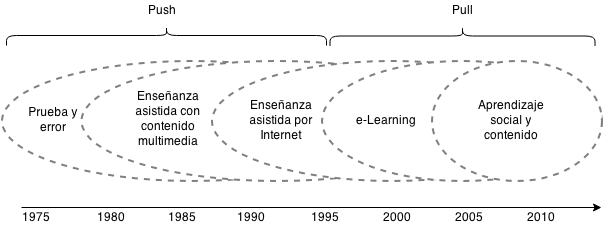
\includegraphics[scale=0.75]{tics/images/tics_history.png}
\caption{Utilización de las \Gls{tic} en la educación desde el año $1975$}
\label{fig:history_tics}
\end{figure}

Para entender la historia de las \Gls{tic} en la educación, se presenta el
gráfico~\ref{fig:history_tics}, en el cual se observa la evolución que sufrió la
utilización de las \Gls{tic} como herramienta en la educación. Se observa que se
parte la historia en cinco corrientes definidas, y a la vez, estas corrientes se
agrupan según el mecanismo de obtención de información, las tres primeras
corrientes se denominan \textit{pull} y las siguientes dos se denominan
\textit{push}. 

\fixme{\textit{Pull} se refiere}{Que es pull? Una corriente? Es la corriente
    pull, los estudian. Obs. Completar la selección} a que los estudiantes
obtenían la información sin participar en la creación de la misma, las
corrientes pedagógicas que marcan tendencias en esta época son el
instruccionismo y el conductismo\cite{white:ict}.

\fixme{\textit{Push} es cuando}{Completar la selección} los alumnos son creados activos de
conocimiento\cite{white:ict,leinonen:ict}, en este periodo de tiempo se
intensifica la creación de herramientas basadas en el constructivismo y el
construccionismo. Es importante notar que las pedagogías de la época
\textit{Pull}, mantienen popularidad y siguen evolucionando, \fixme{solo
    que}{arreglar} a menor medida\cite{white:ict}.

El gráfico~\ref{fig:history_tics} \fixme{muestra}{} el solapamiento entre los diversos
mecanismos utilizados, \fixme{muestra el}{} inicio de la utilización de una herramienta,
pero no su fin, actualmente se sigue utilizando la mayoría de los
enfoques\cite{leinonen:ict}.

Aunque la figura~\ref{fig:history_tics} muestre un progreso lineal de las
corrientes, este progreso no es igual en todo el mundo, y la el grado de
impacto de las \Gls{tic} varia entre países, lo que se conoce como una
\enquote{brecha tecnológica}. \fixme{Las fechas utilizadas en el
    figura~\ref{fig:history_tics} son relacionadas a la evolución en los
    Estados Unidos de Norte America.}{a EE.UU, borrar esto y poner esto en el
    caption}

\observacion{Revisar estructura}
\observacion{Educación, antecedes, instruccionismo?, pero no habla de la
    evolución de instruccionismo, no da a entender en que momento pasa de una a
    otra. Colocar las corrientes en su gráfica 2.1}

\subsection{Instruccionismo}

La educación tradicional o instruccionismo se basa en la transferencia de
conocimiento del profesor al alumno, se enfoca más en el profesor, en la
capacidad del mismo, y en el producto final como resultado de un proceso no
interactivo y bien
documentado\cite{igi:instructionism,johnson2005instructionism}. Los mecanismos
tradicionales para probar la efectividad de este tipo de enseñanza son los
exámenes.

El instruccionismo es conocido además como enseñanza sistemática, enseñanza
explícita, enseñanza directa, y enseñanza activa, siempre enfatizando al
profesor\cite{johnson2005instructionism}.

Epistemológicamente se puede observar al instruccionismo como objetivo, pues
considera que el conocimiento es independiente del entorno, se asume que el
mismo es isomorfo, si el profesor puede enseñar, el alumno puede
aprender\cite{johnson2005instructionism}.

En el instruccionismo, la utilización de las \Gls{tic} en la actualidad se
centra principalmente en mecanismos para proveer contenido, hoy en día se
utilizan plataformas complejas que permiten a los profesores distribuir
contenido y otras actividades relacionadas, estas plataformas se centran bajo
el nombre de \emph{E-Learning}.


\subsubsection{E-Learing} 
\observacion{No se entiende bien la relación entre las corriente pull/push, y
    las corrientes específicas (respecto a su grafo 2.1)}
\observacion{E-Learing, es pull o push. No se refleja bien la relación}

El \emph{E-Learning} se define como la educación y capacitación a través de
medios digitales, incluye todo tipo de medio capaz de distribuir información,
puede ser de en tiempo real como salas de conversaciones y videoconferencias o
puede ser diferido, como por ejemplo foros, enciclopedias. Es particularmente
útil para educación a distancia y con horarios flexibles. Se originó a finales
de la década de $1990$ y tuvo su apogeo a mediados de la década del $2000$,
apoyada por la gran penetración de las \Gls{tic} en la
población\cite{punie:ict}.

Se distribuye contenido masivamente a los alumnos, y luego, de manera discreta
se permite a los mismos colaborar, dejando siempre en claro que primero se debe
asimilar toda la información posible y luego relacionarse con los
demás\cite{leinonen:ict}.


\begin{figure}[h] 
\centering 
\includegraphics[scale=0.5]{tics/images/moodle.jpg}
\caption{Moodle, plataforma de e Learning} 
\label{fig:moodle}
\end{figure}


La plataforma \emph{Moodle} (ver~\ref{fig:moodle}) cuya primera versión salió en
el $2002$, es una de las principales herramientas del \emph{e-Learning} hoy en
día, permite la creación de cursos específicos por materia y sitios
especializados por instituciones académicas\cite{perkins2006using}. 

La utilización del \emph{e-Learning} tiene varios grados de aplicación en
entornos reales\cite{punie:ict}, que van desde ser simples elementos
complementarios a la clase, como por ejemplo un repositorio para las
diapositivas y otros materiales de clase, hasta cursos completamente en línea,
donde la clase ha sido completamente sustituida.

Sí bien, el \emph{e-Learning} permite la distribución y colaboración en
distintos niveles, no hace un enfoque en el aspecto pedagógico, y se centra en
la forma de transmitir información, y no como la recibe el
alumno\cite{leinonen:ict}, tampoco se centra en la reacción del alumno ante la
información recibida, lo que sí es estudiado por el
conductismo\cite{weegar2012comparison}.

\subsubsection{Conductismo}
\observacion{?}
\observacion{Resumir más, balancer las descripciones}

El conductismo es una corriente de la psicología, creada por \textit{Jhon
    Watson}, y posteriormente perfeccionada por \textit{Pavlov},
\textit{Skinner}, y \textit{Thorndik}. El conductismo defiende la idea de que
todas las acciones que realizan los seres vivos son consecuencia de un
estímulo. Un ejemplo de esta técnica es el experimento de \textit{Pavlov},
\fixme{donde un perro es alimentado cada vez que suena una campana, provocando
    que el perro salive cuando suena la campana, incluso si no existe una
    recompensa (alimento)}{algún mejor ejemplo?}\cite{weegar2012comparison}.

\fixme{El conductismo permite a la epistemología utilizar un enfoque
    científico, permitiendo controlar todas las variables controlables, como el
    estímulo y la reacción, e ignorando los pensamientos y experiencias de las
    personas\cite{weegar2012comparison}. }{Traducir en algo más extendible sin
    usar términos como variables controladas, etc.}

La primera incursión del conductismo con las \Gls{tic}, fue presentada por
\textit{Skinner}, en $1958$\cite{weegar2012comparison}, donde se describe una
máquina que contiene botones y una pantalla donde se presenta una pregunta,
para responder el usuario dispone de varias opciones, cada opción esta
relacionada con un botón, si el aprendiz no presiona el botón correcto, debe
seguir intentando hasta acertar y así avanzar\cite{weegar2012comparison}, este
es el inicio de lo que se conoce como \enquote{Prueba y Error}.

Una característica del conductismo, es la ley de \textit{Thorndike}, indica que
una acción cuya consecuencia es un estímulo favorable, es más probable que sea
repetida\cite{weegar2012comparison}, en la
tabla~\ref{tab:conductismo_estimulo}, se observa los distintos mecanismos 
que propone el conductismo para alentar o desalentar un comportamiento.

\begin{table}[!hbt]
\begin{center}
\begin{tabulary}{\textwidth}{|L|C|C|}
\hline
& Comportamiento alentado & Comportamiento reprimido \\
\hline
Estímulo presente & Refuerzo positivo, por ejemplo, buenas notas & Castigo
Presente, por ejemplo, tiempo después de clase \\
\hline
Estímulo eliminado & Refuerzo negativo, por ejemplo, no hacer quehaceres &
Castigo eliminado, por ejemplo, no permitir utilizar la computadora. \\
\hline
\end{tabulary}
\end{center}
\caption{Tipos de estímulos}
\label{tab:conductismo_estimulo}
\end{table}

A finales de la década de $1970$ e inicios de la década de $1980$,  la
complejidad técnica de las computadoras limitaba la cantidad de herramientas
disponibles, los programas eran desarrollados por profesores, y su objetivo era
que los alumnos puedan poner en práctica lo aprendido en el aula. 


El campo de aplicación de las herramientas, basadas en el experimento de
\textit{Skinner}, se limitaban a matemáticas y lenguaje, donde se podía evaluar
inmediatamente los resultados proveídos por los alumnos, pues, normalmente era
un enunciado y una lista posible de opciones del tipo \enquote{Prueba y
    Error}\cite{leinonen:ict}. 

La cantidad limitada de opciones para responder, provocó que los alumnos no
interpreten los resultados, sino prueben todas las posibles opciones hasta
pasar al siguiente enunciado, sin obtener ningún aprendizaje
significativo\cite{leinonen:ict}.

Cuando aparecieron en el mercado computadoras con multimedia, a finales de la
década de $1980$, la utilización de las \Gls{tic} se simplificaron y dieron
contenido a la posibilidad de incluir contenido multimedia, se argumentó que los
ejercicios de tipo \enquote{Prueba y Error} no cumplieron su objetivo de una
educación profunda por que no contenían multimedia\cite{leinonen:ict}, así, en
se empezaron a distribuir las aplicaciones por \textit{CD-ROM} y contener gran
cantidad de contenido multimedia.

Con la creación de los juegos del tipo \enquote{Prueba y Error} y el contenido
multimedia, se inicio a un nueva corriente denominada \emph{Edutainment},
palabra que representa la unión de la educación y el entretenimiento. 

\subsubsection{Edutainment}
\label{sec:edutainment}

\observacion{Esquema Global
\begin{itemize}
    \item Que es?
    \item Quien creo y cuando?
    \item Ejemplos
    \item Fortalezas y desventajas
\end{itemize}
Tratar de hacer las descripciones más simétricas tirando hacia el resumen}

Los \emph{edutainment} se basan principalmente en el conductismo y el
cognoscitivismo, se enfoca en juegos sencillos que transmiten información simple
al usuario, su estructura se basa en un objetivo claro que está separado de la
experiencia educativa\cite{egenfeldt2007third}. 

Así el \emph{edutainment} pretende agregar entretenimiento a la educación, se
ve al alumno como un receptor pasivo de información que debe asimilarla, y para
aumentar la implicación de los alumnos, el entretenimiento era
agregado\cite{resnick:2004}.

\observacion{Conectar mejor \enquote{Un ejemplo es Math Blaster}}

\emph{Math Blaster} (ver~\ref{fig:math_blaster}) es un \emph{edutainment} donde
el alumno debe responder repetitivamente preguntas aritméticas para obtener
municiones, luego con esas municiones debe completar diferentes misiones en una
nave\cite{bruckman1999can}. Como todas las preguntas se responden mediante un
mecanismo de selección múltiple, y no existe penalización por fallar una
respuesta, los alumnos no reflexionan sobre las respuestas elegidas, seleccionan
una opción aleatoria y si no es la correcta, prueban otra, tras una cantidad
finita de intentos, siempre se obtiene la recompensa deseada.

\begin{figure}[ht!] 
\centering 
\includegraphics[scale=0.5,natwidth=296,natheight=217]{tics/images/math_blaster.jpg}
\caption{Math Blaster, \emph{edutainment} del año 1987}
\label{fig:math_blaster} 
\end{figure}

\begin{figure}[ht!] 
\centering 
\includegraphics[scale=0.5]{tics/images/carmen.jpg}
\caption{Donde en el mundo esta Carmen Sandiego} 
\label{fig:carmen}
\end{figure}

\enquote{Donde en el mundo esta Carmen Sandiego} (ver~\ref{fig:carmen}) es un
juego que representa el potencial multimedia de esta época, el objetivo del
juego era detener a una serie de criminales mediante varias pistas que eran
provistas en forma de texto. Este exitoso juego demuestra las falencias del
\textit{Edutainment}, siendo visualmente muy atractivo, y con contenido
multimedia acorde a su tiempo, no era más que \enquote{Prueba y Error}, cada
nivel del juego podía ser completado sin leer la información proveída
educativa\cite{charsky:2010}.

Los \emph{edutainment} no logran enseñar habilidades complejas, se enfocan
principalmente en enseñar tareas extremadamente repetitivas que no dependen de
un contexto\cite{charsky:2010,egenfeldt2007third,bruckman1999can}, son
excelentes para enseñar a sumar, pero no para aplicar ese conocimiento, analizar
y obtener conclusiones, o evaluar lo que aprendieron.

Las principales causas por del fracaso de los \emph{edutainment} en su intento
de ser una alternativa viable a la educación son según\cite{egenfeldt2007third}: 

\begin{itemize}

\item \textbf{Falta de motivación interna:} los \emph{edutainment} se centran en
    motivaciones externas, y dejan de lado la motivación interna. Se centran en
    dar recompensas por acciones lo que es una motivación externa, que en que el
    alumno se sienta emocionado al finalizar un nivel, lo que es una forma de
    motivación interna.

\item \textbf{Aprendizaje como anexo:} el principal objetivo del desarrollo de un
    \emph{edutainment} es el de entretener, los objetivos pedagógicos son
    agregados al final. Adicionalmente, este aprendizaje se provee a través de
    largos textos que normalmente son omitidos.

\item \textbf{Interacción limitada:} son construidos con una jugabilidad pobre,
    sin la posibilidad de realizar multiples acciones, normalmente limitados a
    seleccionar respuestas o moverse en un pequeño mundo. 

\item \textbf{Ejercicios de prueba y error sistemáticos:} todas las debilidades
    anteriores se pueden fundamentar en el hecho de que los juegos permiten al
    alumno intentar varias veces sin ser penalizados, además
    de que los alumnos no están motivados, provocaba que todas las opciones sean
    probadas sin el proceso de reflexión necesario para aprender, por ejemplo,
    varios juegos aritméticos solicitaban pruebas del tipo $2+2$ donde el alumno
    probaba diferentes resultados y luego memorizaba el mismo. Se enseñaba a
    probar opciones sin sentido antes que entender y analizar la experiencia.

\end{itemize}

La distribución por medios físicos, aunque contribuyo a la calidad de material
proveído, no resolvió el problema de información actualizada, pues a comienzos
de la década de $1990$, con la popularización de Internet, se genera más
contenido que el que puede ser distribuido por medios físicos, así se accede al
tercer hito de la figura~\ref{fig:history_tics}, donde el contenido es
distribuido por Internet.

La incursión de internet solo permite contenido actualizado, los problemas
persisten y se crean nuevos factores que ensanchan la brecha tecnológica,
ahora, además de poseer una computadora, es necesaria una conexión permanente.
Adicionalmente, la velocidad inicial de Internet no es suficiente para proveer
los mismos entornos ricos en multimedia que sí lo proveían los
CD-ROM\cite{leinonen:ict}.

\textit{Skinner}, se dio cuenta que el compartimiento humano no puede ser
reducido al conductismo, no solo responde a los estímulos, sino, que además
responde a su experiencia previa\cite{weegar2012comparison}, así se estudia el
constructivismo, que se centra en el alumno y sus experiencias.

\subsection{Constructivismo}

El constructivismo es una corriente pedagógica creada por \textit{Jean Piaget}
y \textit{Lev Vygotsky}, cuya idea central es que el aprendizaje humano se
construye, que la mente de las personas elabora nuevos conocimientos a partir
de la base de enseñanzas anteriores. Predica que el aprendizaje de los
estudiantes debe ser activo, deben participar en actividades en lugar de
permanecer de manera pasiva observando lo que se les
explica\cite{hernandez:constructivismo,johnson2005instructionism}.

El constructivismo es un conjunto de prácticas que se enfocan en el alumno,
basados en el contenido, orientados al proceso, interactivos y que responden a
las necesidades e intereses personales de los
alumnos\cite{johnson2005instructionism}.

Se basa en que las personas no entienden, ni utilizan de manera inmediata la
información que se les proporciona, en cambio, el individuo debe
\enquote{construir} su propio conocimiento. El conocimiento se construye a
través de la experiencia y esto conduce a la creación de modelos mentales que
se almacenan en la mente. Estos esquemas van \fixme{cambiando}{}, ampliándose y
volviéndose más \fixme{sofisticados}{Complejo} a través de dos procesos
complementarios: la asimilación y el
alojamiento\cite{hernandez:constructivismo,johnson2005instructionism}.

Epistemológicamente el constructivismo es subjetivo, pues considera que el
conocimiento depende las experiencias\cite{johnson2005instructionism}. 

Las aulas construccionistas crean un mundo realista donde lo más importante es
el aprendizaje el profesor es un facilitator del aprendizaje del
alumno\cite{johnson2005instructionism,nanjappa2003constructing}.

Actualmente, los cursos de \textit{E-Learing}, tradicionalmente conductistas,
están evolucionando para incluir conceptos
constructivistas\cite{weegar2012comparison}, especialmente donde se requiere de
pensamiento de alto nivel\footnote{Del Inglés, \textit{High Order Thinking},
    incluye la capacidad de resolver problemas complejos, y criterios de
    decisión.}, cuya obtención es vista como una estrategia de actividades
necesarias para conseguir objetivos\cite{miri2007purposely}.

Así, las aplicaciones del constructivismo con las \Gls{tic}, es variado,
incluyendo al \textit{E-Learing} y a los \textit{Edutainment}, hasta lo que hoy
se conoce como \textit{Juegos Serios}, los cuales son descritos en el
capítulo~\ref{chap:juegos_serios}. Otros ejemplos de aplicaciones del
constructivismo, son las \textit{wikis}, redes sociales y los
\textit{blogs}\cite{hernandez:constructivismo}.

Las teoría de \enquote{construccionismo} de \textit{Seymourt Papert},
construida sobre el constructivismo, que agrega, entre otras cosas, la
entorno en la que ocurre el aprendizaje\cite{egenfeldt2007third}, permite
explorar más contenido, proveyendo un punto inicial, y permitiendo explorar
posibles soluciones.

\section{Construccionismo y las TIC}

El construccionismo utiliza la tecnología como medio cognitivo  a diferencia de
la educación tradicional que la utiliza para la entrega de contenido. 

El construccionismo es un alternativa prometedora a la educación
tradicional.Desde el punto de vista tecnológico, el contruccionismo es ideal
pues el mismo requiere un alto dinamismo en el traspaso del conocimiento
\cite{sasha:construtivism}. 

El contruccionismo y las \Gls{tic} siempre han estado relacionados, ya que el
mismo se origino con un lenguaje de programación(LOGO)\cite{ict:ttc}. Un
característica importante de esta relación es que tienen la capacidad de
eliminar los problemas de distancia\cite{mariluz:seiousgames}.


\subsection{Historia}

Seymour Papert adoptó el término construccionismo en la década de 1980 para
representar una método pedagógico practicado por John Dewey a principios del
siglo 20. Este método buscaba que la responsabilidad de aprender recaiga en el
estudiante. 

Papert trabajó directamente con el psicólogo evolutivo y filósofo suizo Jean
Piaget, quién elaboro sus teorías de la educación y construcción del
conocimiento al ver e interactuar con los niños. A partir de esta observación
nació el constructivismo según el cual el conocimiento debe ser construido por
el estudiante y los nuevos significados deben ser obtenidos relacionándolos con
significados anteriores por los mismos estudiantes haciendo uso así de sus
propios sistemas de relaciones.

El construccionismo se diferencia de lo anterior en que los estudiantes
construyen las ideas o partes del mundo utilizando herramientas. La elaboración
de representaciones mentales mediante la construcción y el intercambio es la
metáfora del marco contruccionista. 

Durante 1980, Seymor Papert, Wally Feurzeig, Marvin Minsky y John McCarthy y los
miembros del Departamento de Inteligencia Artificial del \Gls{mit} y una
compañía de tecnología en Cambridge, Massachusetts, desarrollaron un nuevo
lenguaje de programación llamado LOGO que tenía por objeto que los estudiantes
construyeran sus modelos en notación LOGO\@. Este juego introduciría de forma
natural las ideas de los procedimientos, funciones, variables, recursividad, la
modularidad, entre otros.

La creación del lenguaje de programación LOGO dio inicio al construccionismo.

Los desarrolladores de LOGO alentaron el uso de la tecnología para la promoción
de nuevas formas de aprendizaje diferentes a las tradicionales. Las comunidades
que adoptaron al contruccionismo con la creación del lenguaje LOGO fueron en su
mayoría aquellas integradas por ingenieros informáticos y matemáticos
\cite{historia:2014}.

\subsection{Bases Pedagógicas}

Para el construccionismo, el conocimiento es construido por el estudiante en
lugar de ser trasmitido por el profesor\cite{moses:2003} y esto sucede
particularmente cuando el mismo se compromete en la elaboración de un producto o
artefacto que tenga un significado y pueda ser compartido\cite{valdivia:sg}. De
esta manera, se permite a los estudiantes elaborar sus propias interpretaciones
razonadas del mundo mediante la interacción con el mismo.

Según Papert, los alumnos estarán mucho más involucrados en su aprendizaje si
construyen artefactos que los demás pueden ver, criticar y tal vez utilizar. Y
además, el alumno se enfrenta a problemas complejos con estas construcciones,
harán el esfuerzo por resolver problemas y aprender ya que la construcción les
motivará\cite{const:vs}.

El enfoque construccionista establece que los seres humanos conocen y aprenden
de formas diferentes por lo tanto, no se puede elaborar una jerarquía de estilos
de aprendizajes\cite{valdivia:sg}.

\subsection{Estado del Arte}

El construccionismo pone énfasis en el \emph{Aprender haciendo}, esta idea
mejora la práctica educativa tradicional o instruccionismo. 

Existen varios emprendimientos o \emph{amigos del contruccionismo}, para la
mayoría de ellos las computadoras son esenciales mientras que para otros el
mayor esfuerzo está en la incorporación de la tecnología en su práctica
educativa~\cite{papertian:const}.

Algunos de estos emprendimientos son:

\begin{description}

\item[Lenguaje de programación LOGO] El lenguaje Logo es la cuna del
	construccionismo, se basa en el principio de que se aprende mejor
	haciendo, pero se aprende todavía mejor si combina la acción con la
	verbalización  y la reflexión acerca de lo que se ha hecho.

\item[Simulación] La simulación de entornos virtuales brinda a los estudiantes
	la posibilidad de experimentar en un entorno controlado, y de esta
	manera les brinda la posibilidad de poner en práctica sus conocimientos
	sin correr riesgos.

\item[Serious Games] Diseñado con el propósito de aprender. Generalmente hace
	uso de la simulación para permitir un aprendizaje más realista.

\item[Lego Serious Play] Es una iniciativa de Lego que busca fomentar el
	pensamiento creativo por medio de la construcción por parte de los
	estudiantes de su identidad y experiencias utilizando legos. 

\item[\Gls{olpc}]. El esfuerzo se centra en dotar a los niños de una computadora
	duradera, accesible y potente en los países en desarrollo, se dice que
	es un descendiente directo del construccionismo. Con esto se busca que
	la computadora personal sea utilizada como un laboratorio intelectual y
	un vehículo para la auto-expresión. OLPC no tiene que ver con la
	escolarización o la escuela, más bien las utiliza como medio de
	distribución de las computadoras a los niños, los cuales pueden
	utilizarlas para aprender en cualquier lugar y momento. Se busca
	fomentar el aprendizaje natural, es decir, aquel aprendizaje sin
	enseñanza\cite{papertian:const}.

\item[Fabricación personal] Neil Gershenfeld, colega de Papert en el Media Lab
	del \Gls{mit} enseñó un curso titulado \emph{Cómo hacer casi cualquier
		cosa}. La idea se centra en la creación de tecnología que se
	necesita para resolver los problemas que se poseen. Papert no sólo
	defendió la idea de que los niños posean computadoras personales, sino
	también que a la larga ellos debían mantenerlas, repararlas e incluso
	construirlas~\cite{papertian:const}.

\end{description}

%http://constructingmodernknowledge.com/cmk08/wp-content/uploads/2012/10/StagerConstructionism2012.pdf

\subsection{Serious Games y Simulación}

\subsubsection{Serious Games}

Un \emph{Serious Game} es un vídeo juego elaborado con el propósito primario que
no es el de entretener\cite{sg:aoverview}, sino tienen una finalidad educativa
explícita y cuidadosamente pensada, utiliza la tecnología y los conceptos de la
industria de los vídeo juegos para encontrar solución a problemas reales. Es
decir, se utilizan para definir los juegos que poseen una pedagogía incrustada,
algún tipo de evaluación ya sea interna o externa y lo que hay que aprender
(contenido) integrado\cite{damien:sg}.

Los \emph{Serious Game} proveen una oportunidad muy importante para enseñar y
desarrollar profesionales, por que ayudan a crear el tipo de educación que los
adultos prefieren, proveen mecanismos para que los estudiantes cometan errores y
experimenten con sus ideas, con su conocimiento y con la teoría en un ambiente
protegido sin riesgos para la vida o la identidad. 

Los beneficios que brindan los \emph{Serious Game} se acentúan en la medida en
la que los mismos proveen entornos más completos en donde realmente se puedan
poner en práctica la teoría, esto ayuda a una comprensión más profunda del área
de interés.

La principal diferencia entre los \emph{Serious Game} y otras aplicaciones de
\emph{E-Learing} es su enfoque en la creación de una experiencia de aprendizaje
significativo, relevante y atractivo. En un \emph{Serious Game} existen metas
claras de aprendizaje pero las mismas se encuentran en un contexto significativo
en donde se deben aplicar los conocimientos y hacer uso de herramientas que
están a disposición para obtener éxito en la resolución de los problemas
presentados. Estos problemas se equilibran a través de la retroalimentación y
otras estrategias para mantener el interés del estudiante. Todo esto hace que en
los \emph{Serious Game} el principal objetivo sea ganar el juego no aprender,
sin embargo sólo se puede hacer esto dominando el aprendizaje
\cite{papertian:const}.

El campo de los \emph{Serious Game} rechaza la idea de que los profesionales de
la educación pueden ser reemplazados fácilmente, para ellos la labor de estos
profesionales es imprescindible para la reflexión y orientación del aprendizaje.
Es cierto que se puede llegar a aprender sin el apoyo de un profesional de la
educación pero se corre el riesgo de perder el enfoque y la eficacia
\cite{elearning:seiousgames}. 

El \emph{serious Game} no se trata de una modelo de aprendizaje pasajero. Varios
autores como Johan Huizinga, Jean Piaget, Wittgenstin y Seymour Papert han
reconocido su importancia  como objeto de aprendizaje. Los juegos deben ser
elaborados teniendo en cuenta el nivel cognitivo del estudiante, es decir, su
etapa de aprendizaje y en que el aprendizaje difiere de acuerdo a la etapa de
vida en la que se encuentre un estudiante. Mediante la práctica repetida de
actividades relacionadas al área de interés se desarrollan habilidades y
destrezas\cite{education:games}. 

Los siguientes son ejemplos de algunas áreas que utilizan Serious Game:

\begin{description}

\item[Militar] Los primeros juegos a menudo se basaban en lucha o combate.
	Durante más de 30 años los juegos han sido reconocidos como herramientas
	factibles en el entrenamiento de militares. En 1996 se creó un juego
	llamado \emph{Marine Doom} en donde la tarea de los jugadores era el
	aprendizaje de formas de ataque, conservación de municiones. Comunicarse
	con eficacia, dar órdenes al equipo de trabajo entre otros. De esta
	manera tuvo lugar una forma de entrenamiento más atractivo, sin el
	costo, dificultad, riesgos e inconvenientes que implicaría el mismo
	entrenamiento en un entorno real. Además se podían crear situaciones que
	en el mundo real serían muy difíciles de
	replicar~\cite{education:games}.

\item[Salud] Este tipo de juegos son cada vez mayores, los juegos de salud se
	utilizan para la formación de profesionales basada en la simulación. En
	2008 el Centro de Simulación Hollier en Birmingham, Reino Unido, realizó
	una prueba que permitió a médicos jóvenes experimentar y entrenar para
	diversos escenarios médicos a través de maniquíes virtuales como
	pacientes, de este modo el aprendizaje se da por la experiencia. En su
	disertación, Roger D. Smith, realizó una comparación entre la enseñanza
	tradicional y la formación mediante realidad virtual y el uso de
	herramientas basadas en la tecnología de juegos en cuanto a la cirugía
	laparoscópica. Como conclusión afirmó que lo último era más barato,
	requería menos tiempo y que permitió menos errores médicos cuando los
	médicos se presentaban en una cirugía real debido a, entre otras cosas,
	la posibilidad de repetición de la experiencia sin riesgo
	alguno~\cite{education:games}.

\item[Juegos corporativos] Este tipo de juegos se han utilizado para la
	selección de personal, la mejora de comunicación entre los directivos y
	su personal de confianza, y la formación de nuevos empleados. Un ejemplo
	de estos juegos es el INNOV8 de IBM que ayuda en el entrenamiento de los
	estudiantes acerca de la gestión de procesos de negocios. Los Serious
	Game pueden ser utilizados incluso para elaborar planes de
	negocios~\cite{education:games}. 

\end{description}

%\cite{sg:aoverview}\cite{houston:sg}\cite{ibm:seriousgames}
%http://ceur-ws.org/Vol-318/Sanchez.pdf
%http://media.futurelab.org.uk/resources/documents/lit_reviews/Serious-Games_Review.pdf

\subsubsection{Simulación}

La simulación se define como el proceso de diseñar un modelo de un sistema real
y, llevar a cabo experimentos con este modelo, con el fin o bien de entender el
comportamiento del sistema o de la evaluación de distintas estrategias para la
operación del sistema\cite{ingalls2008introduction}. 
%[ingalls2008introduction]

Un juego y una simulación podrían llegar a ser muy parecidos, a veces los juegos
tienen motores de simulación, una de las diferencias es que la simulación es muy
dependiente del contexto. 

Existen dos tipos de simulaciones, en primer lugar están las experimentales que
ponen al estudiante en el lugar de un profesional y requieren que el mismo tome
decisiones para alcanzar los objetivos y en segundo lugar están las simbólicas
que buscan que el estudiante deduzca eventos, principios y mejores prácticas
\cite{charsky:2010}. 
%\cite{charsky:2010}

Una simulación esta conformada por:

\begin{description}

\item[Entidades] Son aquellas que cambian el estado de una silumación, estas
	entidades poseen atributos los cuales son sus características
	exclusivas. Por último, una entidad es cualquier objeto que requiera su
	representación explícita. Ejemplo de entidades son: un médico o una
	jeringa en una simulación médica.

\item[Acciones] Las entidades interactúan entre sí a través de acciones. Estas
	acciones puede causar cambios en el estado de la simulación además de
	eventos. Ejemplo de una acción en una simulación médica es la
	esterilización de un instrumento.

\item[Eventos] Los eventos son hechos que ocurren de manera controlada pero no
	siempre predecible en el entorno simulado, los mismos afectan a las
	entidades y deben obligar a realizar alguna de las acciones disponibles
	para tal evento. Ejemplo de un evento en un simulación médica es un paro
	cardíaco del paciente.

\end{description}

La confianza en el modelo o la simulación según\cite{DoDSysEng2001} se establece
mediante:

\begin{description}

\item[La verificación] Es el proceso de determinar si la implementación
	representa con precisión las especificaciones del diseño. 

\item[La validación] Es el proceso de determinar el grado en el que el modelo
	representa de forma exacta la realidad de acuerdo al uso que se tiene
	previsto darle y el nivel de confianza que debe tenerse en la
	evaluación.

\item[La acreditación] Es el proceso de certificación de un modelo para su uso
	con un propósito específico.
%[DoDSysEng2001]

\end{description}

En la actualidad, es cada vez mayor la utilización de la simulación como
herramienta para el entrenamiento ya que los profesores están más familiarizados
con la tecnología. 

Según\cite{humphreys2013developing} los tipos de estudiantes definidos por Kolb
son:

\begin{description}

\item[Accommodating learners] Aprenden de la experiencia e interiorizan el
	aprendizaje a través de experimentación activa. 

\item[Diverging learners] Aprenden a través de experimentación activa, e
	interiorizan el conocimiento reflexionando sobre la experiencia. 

\item[Coverning learners] Aprenden a través del pensamiento abstracto e
	interiorizan el conocimiento a través de la experimentación activa.

\item[Assimilating learners] Aprenden a través del pensamiento abstracto y las
	interiorizan reflexionando sobre las mismas. 
	
\end{description}

Teniendo en cuenta el caso de la enfermería, la misma es una ciencia que atrae a
alumnos del tipo \emph{Diverging learners}, y la simulación es una herramienta
ideal para este tipo de estudiantes.

La mayoría de la literatura encontrada acerca de la simulación y los cuidados de
salud no proporcionan muchos detalles acerca de la implementación de modelos en
áreas amplias, se cree que esto se debe a la complejidad de representar las
actividades relacionas al cuidado de la salud dentro de un modelo de simulación
que debe, de hecho, ser una simplificación de las mismas. Esta simplificación
puede ser un proceso sumamente complejo, por lo cual la mayoría se centra en una
parte de las actividades hospitalarias pero no así en todas. Cuanto mayor sea el
detalle, la simulación conducirá a una representación más realista lo cual
aumenta la confianza en los grupos de interés, sin embargo, más detalle requiere
más datos validados y esto puede ser costoso de obtener\cite{guna:simulation}.

Algunas aplicaciones específicas en el cuidado de la salud son:

\begin{description}

\item[Departamento de emergencia y accidentes] La mayoría de los trabajos
	realizados en esta área se refieren a la optimización de tiempo de
	espera de los pacientes y la organización del personal, de las
	habitaciones,de las ambulancias, para dar mejor atención a los
	pacientes. Un ejemplo de esto es Edsim que que se utiliza para aumentar
	el rendimiento en un departamento de emergencias en EE.UU como parte de
	un sistema que permite el desvío de ambulancias en los períodos pico de
	demanda, el cual incluye la introducción de salones de descarga y la
	disminución del tiempo de estancia\cite{guna:simulation}. 
	
\item[Instalaciones para pacientes hospitalizados] Los trabajos se centran en la
	mejora en la atención con respecto al flujo de pacientes así como la
	ocupación de camas. Muchos trabajos tratan de demostrar como se podrían
	utilizar modelos matemáticos para esto. Harper y Shahani presentaron un
	modelo de simulación flexible relacionado a estás cuestiones de
	pacientes hospitalizados, el mismo utiliza TOCHSIM, flexible en el
	sentido de que aborda también problemas como la creación de una nueva
	unidad en el hospital\cite{guna:simulation}.

\item[Clínicas para pacientes ambulatorios] En este sentido la simulación se
	utiliza para minimizar el tiempo de espera de los pacientes en clínicas
	externas, es decir, aquellas en las que se sacan citas. El tiempo de
	espera no sólo implica la espera dentro de la clínica sino también el
	tiempo que pasa entre el momento en el que se solicita un cita y el día
	de la cita. Un ejemplo de esto es CLINSIM que se utilizó en el Reino
	Unido para observar como la política de operación puede influir en los
	tiempos de espera de los pacientes\cite{guna:simulation}. 

\item[Formación medica y quirúrgica] Se centran en tareas específicas y en la
	formación de un conjunto limitado de habilidades referentes a estas
	tareas. Los ejemplos más recientes son entrenamiento para un intubación
	esofágica, capacitación y evaluación de capacidades laparoscópicas,
	entrenamiento para la palpación de tumores de mama\cite{mantovani:vr}. 

\item[Sistemas de formación de emergencias] Se refieren a aquellas simulaciones
	diseñadas para la rápida respuesta médica. Incluye desde pacientes
	virtuales dinámicos cuya acción por parte del estudiante produce un
	cambio clínico en el mismo y una respuesta al estudiante.  Otro ejemplo
	es el utilizado en la marina de EE.UU que intenta formar a los
	profesionales para su rápida acción frente a desastres civiles y donde
	la estabilización de pacientes se tenga que dar con recursos
	limitados~\cite{mantovani:vr}. 

\item[Entrenamiento para profesionales de salud mental] Janssen LP creó una
	simulación para educar a los psiquiatras y profesionales de la salud en
	lo que es tener esquizofrenia llamada \emph{el viaje en autobús} que
	trata de mostrar lo que pasa dentro de de la mente de una persona con
	esquizofrenia cuando viaja en autobús en base a experiencias relatadas
	por pacientes y médicos\cite{mantovani:vr}. 

\end{description}


\section{Ventajas y desafíos}
\label{sec:tics_ventajas}

Durante la historia de las \Gls{tic} en la educación, se han encontrado
diferentes dificultades a la hora de aplicar los nuevos conceptos en la
educación, desde los primeros enfoques que carecían de bases pedagógicas válidas
hasta la actualidad, el principal problema es falta de motivación de los
profesionales de la educación para emplear las
\Gls{tic}\cite{punie:ict,ict:romeo}.

%\todox{Reconsiderar el párrafo que esta comentado bajo este todo}
%\fixme{El contenido proveído actualmente puede ser considerado como un conjunto
%    de buenas prácticas\cite{punie:ict} y así, omiten completa o parcialmente el
%    contexto donde esa buena práctica fue generado. }{No se entiende de donde
%    sale esto, de que habla y para qué?}

Aún así, las \Gls{tic} han tenido un impacto positivo en la educación, pero el
mismo no es el esperado\cite{punie:ict}, por ejemplo, iniciativas como el
\emph{edutainment} que prometían ser la solución a los problemas
educacionales no cumplieron las expectativas.

Sucesivos fracasos en los resultados obtenidos dotaron a los \emph{edutainment}
de una reputación negativa, y hoy en día son considerados como un método educativo 
ineficiente, pues son un ejercicio de \emph{prueba-error} ocultos bajo un juego poco 
entretenido, además de su incapacidad de enseñar como aplicar conceptos aprendidos 
a un entorno real\cite{resnick:2004}.

Mientras que la utilización de las \Gls{tic} puede eliminar problemas actuales
como el aislamiento y la falta de pensamiento de alto nivel\cite{punie:ict}, la
brecha social existente implica otro riesgo para la utilización de las \Gls{tic}
en la educación, aquellos que no posean los recursos económicos necesarios para
acceder a la misma no se verán beneficiados por las \Gls{tic}\cite{punie:ict}.

Las empresas involucradas en el área de las \Gls{tic} en
educación siguen en la época donde los juegos son prueba y error, esto no
significa que los mismos no funcionen, sino que pueden ser mejorados
considerablemente\cite{egenfeldt2007third}.

Otro de los desafíos actuales es la dificultad comercial impuesta por la
historia de los mismos, es muy difícil para los juegos actuales presentar
promesas realistas, principalmente por el antecedente sentado por los
\emph{edutainment}\cite{egenfeldt2007third}

Las principales ventajas de la utilización de las \Gls{tic} en la educación son:

\begin{itemize}

\item \textbf{Nuevos modelos pedagógicos:} teorías como el constructivismo moderno
    enfatizan el proceso de como adquirir (aprendizaje) conocimiento y no
    solamente como transmitir el conocimiento en sí
    (enseñanza)\cite{guenaga2013serious}.

\item \textbf{Eliminación de distancias:} Con la aparición de las computadoras y los
    satélites,  el mundo se ha convertido en una aldea global, y las distancias
    en cuestiones de transmisión de información se han vuelto
    insignificantes\cite{mohammed2013information},  los medios tradicionales
    como bibliotecas, o escuelas están limitados a un espacio  físico, con el
    uso de las \Gls{tic}, esta restricción física desaparece\cite{tinio:ict}.

\item \textbf{Colaboración distribuida:} como consecuencia del punto anterior, los
    alumnos pueden colaborar de manera más sencilla pues no tienen limitaciones
    físicas. Además, los alumnos pueden consultar con expertos que están en
    linea, e incluso tener mentores en linea, estas tutorías pueden ser uno a
    uno, por ejemplo mediante comunicaciones por correo electrónico. Además
    permite la colaboración masiva entre estudiantes de intereses comunes,
    mediante foros y redes sociales\cite{unesco:ict}.

\item \textbf{Motivación para aprender:} Las \Gls{tic} tienen un impacto positivo en el
    proceso de aprendizaje especialmente en lo referente al compromiso
    con\cite{passey2004motivational,egenfeldt2007third}:
	    
    \begin{itemize}
    \item \textbf{La actividad}: a través de estímulos visuales, auditivos, etc.
    \item \textbf{La capacidad de investigación}: es más fácil acceder a gran cantidad de
        información bibliográfica.
    \item \textbf{La capacidad de escritura y lectura}: emitiendo compartir  ideas de
        manera más legible y mejorarlas iterativamente.
    \item \textbf{La capacidad de presentación}: es más fácil presentar trabajos
        profesionalmente a un público mayor.
    \end{itemize}
	    
\item \textbf{Adquisición de habilidades básicas:} las habilidades necesarias para
    utilizar de manera efectiva las \Gls{tic} se están convirtiendo en una
    necesidad básica, un aprendizaje guiado por las mismas puede ayudar a una
    rápida asimilación de los conceptos relacionados.

\end{itemize}

Uno de los desafíos más importantes que enfrentan las \Gls{tic} para convertirse
en una alternativa viable es la inversión en infraestructura
necesaria\cite{unesco:ict}.




% Nueva organización
% 
%  Introducción
%  Evolución
%   Antecedentes
%   Instruccionismo
%   Behaviourism
%   Constructivismo
% Construccionismo
% Ventajas y desafíos

%! TEX root = ../main.tex
\chapter{TIC's en la Educación}
\label{chap:tics}

\observacion{Enfocar desde un marco común (tendencias)}

Las \Gls{tic} son un conjunto de herramientas tecnológicas y recursos utilizados
para comunicar, crear, diseminar, almacenar y manejar la
información\cite{unesco:ict}. Estas tecnologías abarcan computadoras personales,
internet, radio, televisión y telefonía\cite{tinio:ict}.

Las \Gls{tic} fueron utilizadas como complemento a la educación desde los
inicios de la misma con la radio y la televisión. Fueron vistas como un
complemento a las herramientas utilizadas en clase, como complemento del libro,
o como una herramienta que elimina la distancia física entre el profesor y el
alumno\cite{unesco:ict}. 


\section{Educación Tradicional}

La educación tradicional o instruccionismo se basa en el concepto de que existe
un profesor y un alumno. El profesor transfiere el conocimiento que ha adquirido
de diferentes métodos (educación, experiencia, etc) a un alumno que es un
receptor pasivo de información\cite{johnson2005instructionism}.

Se enfoca más en el profesor, en la capacidad del mismo, y en el producto final
como resultado de un proceso no interactivo y bien
documentado\cite{igi:instructionism}. Los mecanismos tradicionales para poder
probar la efectividad de este tipo de enseñanza son los exámenes.

La principal critica a este modelo es que se enfoca la enseñanza y no el
aprendizaje, mientras más se enseña, más se aprende. Esto contradice al sentido
común en el sentido de que, cosas básicas como caminar o hablar, aprendemos sin
la necesidad de un
profesor\cite{ackoff:education}\cite{johnson2005instructionism}.

Tradicionalmente el rol de las TIC's en la educación se vio relegada a la de
sustituto del libro y/o de presentaciones en clase, es decir, es un mecanismo
más para trasmitir el conocimiento del maestro al alumno.



\section{Educación con TIC's}
\label{sec:tics_EDUCACION_TICS}

Las expectativas iniciales acerca del impacto de las \Gls{tic} en la educación
fueron ampliamente superiores a los resultados obtenidos\cite{unesco:ict}, con
el advenimiento de las computadoras esta brecha se redujo, en mayor medida por
que se las utilizo en conjunto con tecnologías como Internet, y los efectos
positivos en la educación fueron aumentando gradualmente\cite{unesco:ict}.

Las principales ventajas de la utilización de las \Gls{tic} en la educación es
su aplicabilidad en áreas que no pueden ser cubiertas por otras alternativas,
como son:

\begin{description}

    \item[Nuevos modelos pedagógicos] teorías como el constructivismo moderno
	    enfatizan el proceso de como adquirir conocimiento y no solamente el
	    conocimiento en sí.

    \item[Eliminación de distancias] Con el advenimiento de las computadoras y los
	    satélites, el mundo se ha convertido en una aldea global, y las
	    distancias en cuestiones de transmisión de información se han vuelto
	    insignificantes\cite{mohammed2013information}, los medios
	    tradicionales como bibliotecas, o escuelas están limitados a un
	    espacio físico, con el uso de las \Gls{tic}, esta restricción
	    física desaparece\cite{tinio:ict}.

    \item[Colaboración distribuida] como consecuencia del punto anterior, los
	    alumnos pueden colaborar de manera más sencilla pues no tienen
	    limitaciones físicas. Además, los alumnos pueden consultar con
	    expertos que están en linea, e incluso tener mentores en linea,
	    estas tutorías pueden ser uno a uno, por ejemplo mediante
	    comunicaciones por correo electrónico. Además permite la
	    colaboración masiva entre estudiantes de intereses comunes, mediante
	    foros y redes sociales\cite{unesco:ict}.

    \item[Motivación para aprender] Las \Gls{tic} tienen un impacto positivo en
	    el proceso de aprendizaje especialmente en lo referente al
	    compromiso con la actividad (a través de estímulos visuales,
	    auditivos, etc), capacidad de investigación (es más fácil acceder a
	    gran cantidad de información bibliográfica), capacidad de escritura
	    y lectura (permitiendo compartir ideas de manera más legible y
	    mejorarlas iterativamente) y capacidad de presentación (es más fácil
	    presentar trabajos profesionalmente a un público
	    mayor)\cite{passey2004motivational}\cite{egenfeldt2007third}.

    \item[Adquisición de habilidades básicas] las habilidades necesarias para
	    utilizar de manera efectiva las \Gls{tic} se están convirtiendo en
	    una necesidad básica, un aprendizaje guiado por las mismas puede
	    ayudar a una rápida asimilación de los conceptos relacionados.

\end{description}

Uno de los desafíos más importantes que enfrentan las \Gls{tic} para convertirse
en una alternativa viable es la inversión en infraestructura
necesaria\cite{unesco:ict}. 

\subsection{Historia}

La historia de las \Gls{tic} en educación comienza con la Universidad Abierta
del Reino Unido\footnote{Open University of United Kingdom} que en 1969 se
establece como la primera institución educativa dedicada a la enseñanza a
distancia utilizando las, para aquel entonces, nuevas
tecnologías\cite{tinio:ict}.

En 1973 Vint Cerf creo el protocolo TCP/IP y es considerado el nacimiento de
Internet\cite{white:ict}, lo que permitió que la información pueda ser
transmitida de manera más sencilla, tiempo después con la aparición de las
computadoras personales en 1977\cite{white:ict}. 

Otro hito tecnológico se dio en la \Gls{cern} en el año 1989 cuando se concibió
lo que hoy se conoce como \emph{World Wide Web}, permitiendo que los usuarios de
la \emph{Web} puedan compartir archivos mediante un protocolo
estándar\cite{white:ict}. 

Con las principales eventos que marcaron la evolución tecnológica de las
\Gls{tic} en la educación, se divide su historia en cinco partes. Las mismas se
pueden dividir en dos secciones, las primeras tres corresponden a los comienzos
y donde los alumnos eran receptores de información, época denominada
\emph{pull}, y la segunda denominada\emph{push}\cite{white:ict} que es aquella
donde los alumnos participan de su educación y son creadores activos de
conocimiento.

\subsubsection{Programación, ejercicios y prácticas}

Este periodo que abarca desde la aparición de las primeras computadoras
personales hasta el final de la década de 1980, este periodo se caracterizo por
computadoras muy limitadas, ausencia de interacción multimedia y escasez de
programas especializados. Se enseñaba programación básica\cite{leinonen:ict}, no
por la necesidad de educar programadores, sino por la creencia de que así se
desarrollarían habilidades matemáticas y lógicas en los alumnos. 


\subsubsection{Edutainment}
\todox{Debería ser un nivel más anidado.}

En este periodo se desarrollaron una gran cantidad de aplicaciones educativas
que más tarde serían conocidas como \emph{Edutainment}\footnote{Education +
	Enteirtainment, se traduce como educación entretenida}, estas pretendían
agregarle entretenimiento a la educación, se veía al como un receptor pasivo de
información que debía asimilarla, y para aumentar el compromiso, el
entretenimiento era agregado\cite{resnick:2004}.

Esta basado principalmente en la teoría del conductismo y el cognoscitivismo, se
enfoca en juegos sencillos que transmiten información simple al usuario, siendo
este un receptor pasivo de información, su estructura se basa en un objetivo
claro que esta separado de la experiencia educativa\cite{egenfeldt2007third}.
Math Blaster (ver~\ref{fig:math_blaster}) es un \emph{edutainment} donde el
alumno debe responder repetitivamente preguntas aritmeticas para obtener
municiones, luego con esas municiones debe completar diferentes misiones en una
nave\cite{bruckman1999can}. Como todas las preguntas se responden mediante un
mecanismo de selección múltiple, y no existe penalización por fallar una
respuesta, rapidamente los alumnos seleccionan cualquier opción, si no es la
correcta, eligen la siguiente, y repiten el proceso hasta obtener la respuesta
correcta, este proceso es conocido como \emph{prueba y error sistemático}. 

\begin{figure}[h!] 
	\centering 
	\includegraphics[scale=0.5,natwidth=296,natheight=217]{tics/math_blaster.jpg}
	\caption{Math Blaster, \emph{edutainment} del año 1987}
	\label{fig:math_blaster} 
\end{figure}

Los \emph{edutainment} fallaron en enseñar habilidades no triviales, se enfocan
principalmente enseñar tareas extremadamente repetitivas que no dependen de un
contexto\cite{charsky:2010}\cite{egenfeldt2007third}\cite{bruckman1999can}, son
excelentes para enseñar a sumar, pero no para aplicar ese conocimiento, analizar
y obtener conclusiones, o evaluar lo que aprendieron.

Las principales causas por las cuales los \emph{edutainment} fracasaron en su
intento de ser una alternativa viable a la educación son según
\cite{egenfeldt2007third}: 

\begin{description}

    \item[Falta de motivación interna] la única forma que tenían de intentar que
	    el alumno quiera seguir jugando eran las recompenzas, que eran muy
	    seguidas y fáciles de conseguir.

    \item[Aprendizaje como anexo] el principal objetivo del desarrollo de los
	    \emph{edutainment} eran el de entretener, los objetivos pedagógicos
	    eran agregados al final. Se enviaban informaciones al alumno
	    mediante largos textos que normalmente eran omitidos.
    
    \item[Jugabilidad sencilla] la mayoría eran sencillos juegos de arcade, la
	    mayor parte de la interacción eran a traves de palabras que eran
	    presentadas en forma de selección multiple. 

    \item[Ejercicios de prueba y error sistemáticos] todas las debilidades
	    anteriores se pueden fundamentar en el hecho de que los juegos
	    permitían al alumno intentar varías veces antes de dar una opción
	    correcta, sumando esto al echo de que los mismos no estaban
	    motivados, provocaba que todas las opciones sean probadas sin el
	    proceso de reflexión necesario para aprender, por ejemplo, varios
	    juegos aritméticos solicitaban pruebas del tipo
	    \begin{math}{2+2}\end{math} el alumno probaba diferentes resultados
	    y luego memorizaba el mismo. Se enseñaba a probar opciones sin
	    sentido antes que entender y analizar la experiencia.

\end{description}

\subsubsection{Entrenamiento basado en computadoras}

Cuando aparecieron en el mercado computadoras con multimedia, se argumento que
los ejercicios de la era anterior fallaron en su objetivo de una educación
profunda por que no contenían multimedia\cite{leinonen:ict}, las aplicaciones
eran distribuidas por CD-ROM, y así se actualizaban de manera más frecuente, y
podían contener gran cantidad de contenido multimedia.

Las bases pedagógicas de esta se basada en la capacidad de ciertos estudiantes
de aprender mejor cuando interactúan con contenido multimedia, la \emph{prueba y
	error} aún estaban presentes, pero no eran presentados inmediatamente,
sino más bien una vez que el alumno ya debería haber asimilado los conceptos y
funcionaban como pruebas de adquisición de conocimiento. Este tipo de contenido
tampoco logro la enseñanza profunda, solamente fueron efectivos en el
aprendizaje de idiomas, fallando en todos los demás campos\cite{leinonen:ict},
además los contenidos muchas veces estaban desactualizados y obtener nuevas
versiones no era una tarea sencilla.

Varios gobiernos apoyaron de manera agresiva la introducción de las \Gls{tic} en
educación\cite{mcdougall2006theory} y se realizo un importante avance teórico
con los trabajos sobre el aprendizaje construccionista de Papert y Harel (1991),
y la influencia de las computadoras sobre el aprendizaje y la mente de Marvin
Minksy (1987)~\cite{mcdougall2006theory}.

A comienzos de la decada de 1990, con la popularización de Internet, se le vio
como solución al problema de las poco frecuentes actualizaciones de aplicaciones
educativas, su utilización no tenia bases pedagógicas, más bien se basaban en la
facilidad de distribuir contenido por la \emph{Web}, el principal inconveniente
era la velocidad del Internet, no era suficiente para proveer entornos ricos en
multimedia como lo hacían los CD-ROM\cite{leinonen:ict}.

\begin{figure}[ht!] 
	\centering 
	\includegraphics[scale=0.5]{tics/carmen.jpg}
	\caption{Donde en el mundo esta Carmen Sandiego} 
	\label{fig:carmen}
\end{figure}

Donde en el mundo esta Carmen Sandiego (ver~\ref{fig:carmen}) es un juego que
representa el potencial multimedia de esta época, el objetivo del juego era
detener a una serie de criminales mediante una serie de pistas que eran
provistas en forma de texto\cite{charsky:2010}. Este exitoso juego demuestra las
falencias de esta época, siendo visualmente muy atractivo, y con contenido
multimedia acorde a su tiempo, no era más que prueba y error, cada nivel del
juego podía ser completado sin leer el texto que contenía la información
educativa.

Todos los errores cometidos en la época anterior estaban presentes nuevamente,
no se establecieron marcos teóricos que fundamentasen la utilización de
contenido multimedia, así, se solucionaron los problemas de simplicidad, pero se
demostró que el principal problema era la prueba y error sistemático y sin
sentido\cite{egenfeldt2007third} 

\subsubsection{e-Learning}

La bases pedagógicas de esta son similares a la era del entrenamiento basado en
computadoras, se distribuye contenido masivamente a los alumnos, y luego, de
manera muy discreta se permite a los mismos colaborar, dejando siempre en claro
que primero se debe asimilar toda la información posible y luego relacionarse
con los demás\cite{leinonen:ict}.

\emph{E-Learning} se define como la educación y capacitación a traves de medios
digitales, incluye todo tipo de media capaz de distribuir información, puede ser
síncrono o asíncrono, y es particularmente útil para educación a distancia y con
horarios flexibles. Se origino a finales de la década de 1990 y tubo su apogeo a
mediados de la década del 2000, apoyada por la gran penetración de las \Gls{tic}
en la población\cite{punie:ict}.

Todos los paradigmas anteriores viven dentro del \emph{e-Learning}, permitiendo
compartir contenido multimedia y realizar pruebas del tipo \emph{prueba-error}. 

\begin{figure}[h] \centering \includegraphics[scale=0.5]{tics/moodle.jpg}
	\caption{Moodle, plataforma de e Learning} \label{fig:moodle}
\end{figure}

La plataforma \emph{Moodle} (ver~\ref{fig:moodle}) cuya primera versión salio en
el 2002, es una de las principales herramientas del \emph{e-Learning} hoy en
día, permite la creación de cursos específicos por materia y sitios
especializados por instituciones académicas\cite{perkins2006using}. 

Si bien en las anteriores épocas, el uso de las \Gls{tic} estaba más orientado
hacia la educación básica y secundaría, el \emph{e-Learning} actualmente es más
utilizado en la educación terciaría\cite{punie:ict}.

La utilización del \emph{e-Learning} tiene varios grados de aplicación en
entornos reales\cite{punie:ict}, que van desde ser simples elementos
complementarios a la clase, como por ejemplo un repositorio para las
diapositivas y otros materiales de clase, hasta cursos completamente en linea,
donde la clase ha sido completamente sustituída.

\section{Problemas actuales}

Durante la historia de las \Gls{tic} en la educación, se han encontrado
diferentes dificultades a la hora de aplicar los nuevos conceptos en la
educación, desde los primeros enfoques que carecían de bases pedagógicas válidas
hasta la actualidad, el principal problema es falta de motivación de los
profesionales de la educación para emplear las
\Gls{tic}\cite{punie:ict,ict:romeo}.

\todox{Reconsiderar el párrafo que esta comentado bajo este todo}
%\fixme{El contenido proveído actualmente puede ser considerado como un conjunto
%    de buenas prácticas\cite{punie:ict} y así, omiten completa o parcialmente el
%    contexto donde esa buena práctica fue generado. }{No se entiende de donde
%    sale esto, de que habla y para qué?}

Aún así, las \Gls{tic} han tenido un impacto positivo en la educación, pero el
mismo no es el esperado\cite{punie:ict}, por ejemplo, iniciativas como el
\emph{edutainment} que prometían ser la solución a los problemas
educacionales no cumplieron las expectativas. 

Sucesivos fracasos en los resultados obtenidos dotaron a los \emph{edutainment}
de una reputación negativa, y hoy en día son considerados como un método educativo 
ineficiente, pues son un ejercicio de \emph{prueba-error}
ocultos bajo un juego poco entretenido\cite{resnick:2004}, además de su
incapacidad de enseñar como aplicar conceptos aprendidos a un entorno
real\cite{resnick:2004}.


Mientras que la utilización de las \Gls{tic} puede eliminar problemas actuales
como el aislamiento y la falta de pensamiento de alto nivel\cite{punie:ict}, la
brecha social existente implica otro riesgo para la utilización de las \Gls{tic}
en la educación, aquellos que no posean los recursos económicos necesarios para
acceder a la misma no se verán beneficiados por las \Gls{tic}\cite{punie:ict}.

\fixme{Empresas que están en el área de las \Gls{tic}}{Mejorar/pulir lengua} en
educación siguen en la época donde los juegos son prueba y error, esto no
significa que los mismos no funcionen, sino que pueden ser mejorados
considerablemente\cite{egenfeldt2007third}.

Otro de los desafíos actuales es la dificultad comercial impuesta por la
historia de los mismos, es muy difícil para los juegos actuales presentar
promesas realistas, principalmente por el antecedente sentado por los
\emph{edutainment}\cite{egenfeldt2007third}

\section{Construccionismo y las TIC's}
\label{sec:tics_CONSTRUCCIONISMO}

\fixme{El construccionismo es una corriente}{decir primero que es, antes de
    comprara} pedagógica con un enfoque diferente en cuanto al uso de las
\Gls{tic} en la educación. Esta pedagogía se diferencia de la educación
tradicional en que el estudiante ya no es un receptor pasivo de información, en
cambio, el mismo participa activamente del proceso de aprendizaje construyendo
su propio conocimiento. 

\fixme{El construccionismo}{no repetir} utiliza la tecnología como medio
cognitivo  a \fixme{diferencia}{} de la educación tradicional que la utiliza para la
entrega de contenido. 

\fixme{El construccionismo}{no repetir} es un alternativa prometedora a la
educación tradicional. Desde el punto de vista tecnológico, el construccionismo
es ideal pues el mismo requiere un alto dinamismo en el traspaso del
conocimiento \cite{sasha:construtivism}. 

\fixme{El construccionismo}{no repetir} y las \Gls{tic} siempre han estado
relacionados, ya que el mismo se originó con un lenguaje de programación
(LOGO)\cite{ict:ttc}. Un característica importante de esta relación es que
tienen la capacidad de eliminar los problemas de
distancia\cite{mariluz:seiousgames}.


\subsection{Historia}

En la decada de $1980$, \emph{Seymour Papert} adoptó el término construccionismo
para representar una método pedagógico practicado por \fixme{John Dewey}{?} a
principios del siglo 20. Este método buscaba que la responsabilidad de aprender
recaiga en el estudiante. 

Papert trabajó directamente con el psicólogo evolutivo y filósofo suizo Jean
Piaget. \fixme{Este}{qué?} último, había elaborado con anterioridad sus teorías
de la educación y construcción del conocimiento al ver e interactuar con los
niños y a partir de esta observación dio origen al constructivismo, según el
cual, el conocimiento debe ser construido por el estudiante y los nuevos
significados deben ser obtenidos relacionándolos con significados anteriores por
los mismos estudiantes haciendo uso así de sus propios sistemas de relaciones.

El construccionismo se \fixme{diferencia}{} de lo anterior en que los estudiantes
construyen las ideas o partes del mundo utilizando herramientas. La elaboración
de representaciones mentales mediante la construcción y el intercambio es la
metáfora del marco construccionista. 

Durante $1980$, Seymor Papert, Wally Feurzeig, Marvin Minsky y John McCarthy y los
miembros del Departamento de Inteligencia Artificial del \Gls{mit} y una
compañía de tecnología en Cambridge, Massachusetts, desarrollaron un nuevo
lenguaje de programación llamado LOGO que tenía por objeto que los estudiantes
construyeran sus \fixme{modelos}{que modelos} en notación LOGO@. Este juego
introduciría de forma natural las ideas de los procedimientos, funciones,
variables, recursividad, la modularidad, simulación, verificación, entre otros.

La creación del lenguaje de programación LOGO dio inicio al construccionismo.

Los desarrolladores de LOGO no solo alentaron la promoción de formas
construccionistas de enseñanza y aprendizaje sino también alentaron otra forma
de aprendizaje nueva y no tradicional con las diferentes herramientas tecnológicas. 

De vuelta en la década de 1980, cuando se produjo LOGO y se acuñó el
construccionismo, la comunidad del construccionismo era en su mayoría  ingenieros
informáticos y matemáticos\cite{historia:2014}.

\observacion{Toda la sección hay que reordernar}

\subsection{Bases Pedagógicas}

Para el construccionismo, el conocimiento es construido por el estudiante en
lugar de ser trasmitido por el \fixme{profesor}{explicar el rol del profesor en
    el construccionismo}\cite{moses:2003} y esto sucede particularmente cuando
el mismo se compromete en la elaboración de un producto o artefacto que tenga un
significado y pueda ser compartido\cite{valdivia:sg}. De esta manera, se permite
a los estudiantes elaborar sus propias interpretaciones razonadas del mundo
mediante la interacción con el mismo.

Según Papert, los alumnos estarán mucho más involucrados en su aprendizaje si
construyen artefactos que los demás pueden ver, criticar y tal vez utilizar. Y
además, el alumno se enfrenta a problemas complejos con estas construcciones,
harán el esfuerzo por resolver problemas y aprender ya que la construcción les
motivará\cite{const:vs}.

El enfoque construccionista establece que los seres humanos conocen y aprenden
de formas diferentes por lo tanto, no se puede elaborar una jerarquía de estilos
de aprendizajes\cite{valdivia:sg}.

\subsection{\fixme{Estado del Arte}{Construccionismo en la presente}}

El construccionismo pone énfasis en el \emph{Aprender haciendo}, esta idea
\fixme{mejora}{ref} la práctica educativa tradicional o instruccionismo. El instruccionismo
se basa en el concepto de que existe un profesor y un estudiante, el profesor
transfiere el conocimiento que ha adquirido a un alumno que es receptor pasivo
de información de esta manera, se enfoca más en la capacidad del profesor. 

Existen varios emprendimientos o \emph{\fixme{amigos del contruccionismo}{?}},
para la mayoría de ellos las computadoras son esenciales mientras que para otros
el mayor esfuerzo está en la incorporación de la tecnología en su práctica
educativa\cite{papertian:const}.

Algunos de estos emprendimientos son:

\observacion{Cambiar el ``description'' por ``itemize''}
\begin{description}

\item[Lenguaje de programación LOGO]  A mediados de la década de 1960 Seymour
	Papert, que había estado trabajando con Piaget en Ginebra, llegó a
	Estados Unidos donde co-fundó el Laboratorio de Inteligencia Artifical
	del MIT con Marvin Minsky. Papert trabajó con el equipo de Bolt, Beranek
	y Newman, liderado por Wallace Feurzeig, que creó la primera versión del
	logotipo en 1967. A lo largo de la década de 1970 Logo fuen incubado en
	el MIT y algunos otros sitios de investigación. El lenguaje de
	programación Logo, un dialecto de Lisp, fue diseñado como una
	herramienta para el aprendizaje. Sus características como la
	modularidad, extensibilidad, interactividad y flexibilidad se derivan de
	este objetivo. 
	%http://el.media.mit.edu/logo-foundation/logo/index.html

	El lenguaje Logo es la cuna del construccionismo, se basa en el
	principio de que se aprende mejor haciendo, pero se aprende todavía
	mejor si se combina la acción con la verbalización  y la reflexión
	acerca de lo que se ha hecho. Fundamentalmente consiste en presentar a
	los niños retos intelectuales que puedan ser resueltos mediante el
	desarrollo de programas en Logo. El proceso de revisión manual de los
	errores contribuye a que el niño desarrolle habilidades metacognitivas
	al poner en práctica procesos de auto-corrección\cite{logo:sg}.
	%http://es.wikipedia.org/wiki/Logo_(lenguaje_de_programaci%C3%B3n)

    \observacion{Ver que decir  qu eno sea repetitivo con todo lo que ya se
        dijo.}


%\item[Simulación] La simulación en el ámbito de la educación fue evolucionando
%desde simples motores de reglas hasta complejos entornos, la simulación
%demostró ser una herramienta muy útil el ámbito laboral
%\cite{mariluz:seiousgames}, pues enseña al alumno a encarar situaciones muy
%difíciles de representar en entornos completamente controlados y provee
%mecanismos para comprobar la efectividad de la herramienta. 

%Actualmente la simulación se utiliza más en el ámbito empresarial pues las
%empresas son las más necesitas de innovar en el ámbito de la enseñanza. Un
%ejemplo de esta necesidad se da, por ejemplo, en el entrenamiento de nuevos
%vendedores, es muy difícil enseñar a un vendedor como debe vender los productos
%con un pizzarón y/o una presentación, en cambio la simulación permite que el
%mismo pueda probar cosas nuevas y experiencias de sus compañeros (o
%instructor), convirtiendo así el aprendizaje en
%colectivo\cite{mariluz:seiousgames}. En el ámbito académico la simulación mas
%utilizada en campos físicos (como simulación de fluidos), meteorología
%(simulación de tormentas y fenómenos climáticos), etc. 

%\item[Serious Games] Diseñado con el propósito de aprender. Generalmente hace
%uso de la simulación para permitir un aprendizaje más realista.

%\item[Lego Serious Play] Es una iniciativa de Lego que busca fomentar el
%pensamiento creativo por medio de la construcción por parte de los estudiantes
%de su identidad y experiencias utilizando legos. 

\item[\Gls{olpc}]. El esfuerzo se centra en dotar a los niños de una computadora
	duradera, accesible y potente en los países en desarrollo, se dice que
	es un descendiente directo del construccionismo. Con esto se busca que
	la computadora personal sea utilizada como un laboratorio intelectual y
	un vehículo para la auto-expresión. OLPC no tiene que ver con la
	escolarización o la escuela, más bien las utiliza como medio de
	distribución de las computadoras a los niños, los cuales pueden
	utilizarlas para aprender en cualquier lugar y momento. Se busca
	fomentar el aprendizaje natural, es decir, aquel aprendizaje sin
	enseñanza.

    \fixme{Los problemas atribuidos al experimento}{experimento?} OLPC son
    predominantemente las críticas a la política, el liderazgo o de la
    intransigencia de la escuela en vez del construccionismo o computadora
    personal para los niños pobres. El experimento audaz de Nicholas Negroponte
    (co-fundador de \Gls{olpc}) y Sugata Mitra para dejar las computadoras desde
    un helicóptero sobre una aldea de África se basa en la creencia en el
    construccionismo\cite{papertian:const}.

    \observacion{Poner referencias}
    \observacion{Terrible descripción del proyecto OLPG}
    \observacion{No se de que portal sacaron esta descripción}

\item[Fabricación personal] Neil Gershenfeld, colega de Papert en el Media Lab
	del \Gls{mit} dictó un curso titulado \emph{Cómo hacer casi cualquier
		cosa}. La idea se centraba en la creación de  la tecnología que
	se necesita para resolver los problemas que se poseen. Esta
	auto-confianza, la autonomía personal y la agencia sobre la tecnología
	han estado en el centro de trabajo de Papert durante años. Papert no
	sólo defendió la idea de que los niños posean computadoras personales,
	sino también que a la larga ellos debían mantenerlas, repararlas e
	incluso construirlas.

	Junto con la capacidad para utilizar la tecnología para inventar
	soluciones a los problemas de significado personal, los estudiantes no
	sólo tienen acceso a la información, sino que tienen una mayor capacidad
	para darle forma a su mundo. La fabricación personal promueve la visión
	de Papert \emph{Si se puede utilizar la tecnología para hacer las cosas,
		usted puede hacer las cosas muchos más interesantes y usted
		puede aprender mucho más haciéndolo}\cite{papertian:const}.

\end{description}

%http://constructingmodernknowledge.com/cmk08/wp-content/uploads/2012/10/StagerConstructionism2012.pdf


\section{Simulación}
\label{sec:tics_SIMULACION}

\obervacion{No se entiende como se llego a esto}

\observacion{Ver como organizar el contenido para que no sea una bolsa de
    conceptos}.

La simulación se define como el proceso de diseñar un modelo de un sistema real
y, llevar a cabo experimentos con este modelo, con el fin o bien de entender el
comportamiento del sistema o de la evaluación de distintas estrategias para la
operación del sistema\cite{ingalls2008introduction}. 
%[ingalls2008introduction]

Un juego y una simulación podrían llegar a ser muy parecidos, a veces los juegos
tienen motores de simulación\footnote{Un motor de simulación es un conjunto de
objetos y métodos que se utilizan para la construcción de modelos de
simulación que están dentro de las aplicaciones}, una de las diferencias
es que la simulación es muy dependiente del contexto. 

La simulación en el ámbito de la educación fue evolucionando desde simples
motores de reglas hasta complejos entornos, la simulación demostró ser una
herramienta muy útil en el ámbito laboral\cite{mariluz:seiousgames}, pues enseña
al alumno a encarar situaciones muy difíciles de representar en entornos
completamente controlados y provee mecanismos para comprobar la efectividad de
la herramienta. 

Actualmente la simulación se utiliza más en el ámbito empresarial pues las
empresas son las más necesitadas de innovar en el ámbito de la enseñanza. Un
ejemplo de esta necesidad se da, por ejemplo, en el entrenamiento de nuevos
vendedores, es muy difícil enseñar a un vendedor como debe vender los productos
con un pizarrón y/o una presentación, en cambio la simulación permite que el
mismo pueda probar cosas nuevas y experiencias de sus compañeros (o instructor),
convirtiendo así el aprendizaje en colectivo\cite{mariluz:seiousgames}. En el
ámbito académico la simulación es más utilizada en campos físicos (como simulación
de fluidos), meteorología (simulación de tormentas y fenómenos climáticos), etc. 

Existen dos tipos de simulaciones, en primer lugar están las experimentales que
ponen al estudiante en el lugar de un profesional y requieren que el mismo tome
decisiones para alcanzar los objetivos y en segundo lugar están las simbólicas
que buscan que el estudiante deduzca eventos, principios y mejores prácticas
\cite{charsky:2010}. 

\fixme{Una simulación}{sección?} esta conformada por:

\begin{description}

\item[Entidades] Cualquier objeto o componente en el sistema que requiera
	representación explícita en el modelo se define como
	entidad\cite{banks2000dm}. Las entidades poseen atributos. Los atributos
	son las características de una determinada entidad que son exclusivos de
	esa entidad. Por último, son aquellas que cambian el estado de una
	simulación. Ejemplo de entidades son: un médico o una jeringa en una
	simulación médica.

\item[Acciones] Las entidades interactúan entre sí a través de acciones. Estas
	acciones puede causar cambios en el estado de la simulación además de
	eventos. Ejemplo de una acción en una simulación médica es la
	esterilización de un instrumento.

\item[Eventos] Los eventos son hechos que ocurren de manera controlada pero no
	siempre predecible en el entorno simulado, los mismos afectan a las
	entidades y deben obligar a realizar alguna de las acciones disponibles
	para tal evento. Ejemplo de un evento en un simulación médica es un paro
	cardíaco del paciente.

\end{description}

La confianza en el modelo o la simulación según\cite{DoDSysEng2001} se establece
mediante:

\begin{description}

\item[La verificación] Es el proceso de determinar si la implementación
	representa con precisión las especificaciones del diseño. 

\item[La validación] Es el proceso de determinar el grado en el que el modelo
	representa de forma exacta la realidad de acuerdo al uso que se tiene
	previsto darle y el nivel de confianza que debe tenerse en la
	evaluación.

\item[La acreditación] Es el proceso de certificación de un modelo para su uso
	con un propósito específico.
%[DoDSysEng2001]

\end{description}



%En la actualidad, la utilización de la simulación como herramienta para el
%entrenamiento es cada vez mayor por partes de los profesores, quienes están
%cada vez más familiarizados con la tecnología. 

%Según\cite{humphreys2013developing} los tipos de estudiantes definidos por Kolb
%son:

%\begin{description}

%\item[Accommodating learners] Aprenden de la experiencia e interiorizan el
%aprendizaje a través de experimentación activa. 

%\item[Diverging learners] Aprenden a través de experimentación activa, e
%interiorizan el conocimiento reflexionando sobre la experiencia. 

%\item[Coverning learners] Aprenden a través del pensamiento abstracto e
%interiorizan el conocimiento a través de la experimentación activa.

%\item[Assimilating learners] Aprenden a través del pensamiento abstracto y las
%interiorizan reflexionando sobre las mismas. 
	
%\end{description}

%Teniendo en cuenta el caso de la enfermería, la misma es una ciencia que atrae
%a alumnos del tipo \emph{Diverging learners}, y la simulación es una
%herramienta ideal para este tipo de estudiantes.

La mayoría de la literatura encontrada acerca de la simulación y los cuidados de
la salud no proporcionan muchos detalles acerca de la implementación de modelos
de simulación en áreas amplias, se cree que esto se debe a la complejidad de
representar las actividades relacionas al cuidado de la salud dentro de un
modelo de simulación que debe, de hecho, ser una simplificación de las mismas.
Esta simplificación puede ser un proceso sumamente complejo, por lo cual la
mayoría se centra en una parte de las actividades hospitalarias pero no así en
todas. Cuanto mayor sea el detalle, la simulación \fixme{conducirá}{} a una representación
más realista lo cual aumenta la confianza en los grupos de interés, sin embargo,
más detalle requiere más datos validados y esto puede ser costoso de
obtener\cite{guna:simulation}.

Algunas aplicaciones específicas en el cuidado de la salud son:
\observacion{Incluir un párrafo porque el énfasis en simulación y salud}

\begin{description}

\item[Departamento de emergencia y accidentes] La mayoría de los trabajos
	realizados en esta área se refieren a la optimización de tiempo de
	espera de los pacientes y la organización del personal, de las
	habitaciones,de las ambulancias, para dar mejor atención a los
    pacientes. Un ejemplo de esto es \emph{Edsim} que se utiliza para aumentar
    el rendimiento en un departamento de emergencias en los Estados Unidos como
    parte de un sistema que permite el desvío de ambulancias en los períodos
    pico de demanda, el cual incluye la introducción de salones de descarga y la
    disminución del tiempo de estancia, sin pasar por el
    triaje\cite{guna:simulation}. 
	
\item[Instalaciones para pacientes hospitalizados] Los trabajos se centran en la
    mejora en la atención con respecto al flujo de pacientes así como la
    ocupación de camas. Muchos trabajos tratan de demostrar como se podrían
    utilizar modelos matemáticos para esto. \emph{Harper y Shahani} presentaron
    un modelo de simulación flexible relacionado a estás cuestiones de pacientes
    hospitalizados, el mismo utiliza \emph{TOCHSIM}, \fixme{flexible en el sentido de
        que aborda también}{pulir} problemas como la creación de una nueva
    unidad en el hospital\cite{guna:simulation}.

\item[Clínicas para pacientes ambulatorios] \fixme{En este sentido}{?} la
    simulación se utiliza para minimizar el tiempo de espera de los pacientes en
    clínicas externas, \fixme{es decir}{pulir}, aquellas en las que se sacan citas. El tiempo
    de espera no sólo implica la espera dentro de la clínica sino también el
    tiempo que pasa entre el momento en el que se solicita un cita y el día de
    la cita. Un ejemplo de esto es \emph{CLINSIM} que se utilizó en el Reino
    Unido para observar como la política de operación puede influir en los
    tiempos de espera de los pacientes\cite{guna:simulation}. 

\item[Formación médica y quirúrgica] Se centran en tareas específicas y en la
	formación de un conjunto limitado de habilidades referentes a estas
	tareas. Los ejemplos más recientes son entrenamiento para un intubación
	esofágica, capacitación y evaluación de capacidades laparoscópicas,
	entrenamiento para la palpación de tumores de mama\cite{mantovani:vr}. 

\item[Sistemas de formación de emergencias] Se refieren a aquellas simulaciones
	diseñadas para la rápida respuesta médica. Incluye desde pacientes
	virtuales dinámicos cuya acción por parte del estudiante produce un
	cambio clínico en el mismo y una respuesta al estudiante.  Otro ejemplo
	es el utilizado en la marina de EE.UU que intenta formar a los
	profesionales para su rápida acción frente a desastres civiles y donde
	la estabilización de pacientes se tenga que dar con recursos
	limitados~\cite{mantovani:vr}. 

\item[Entrenamiento para profesionales de salud mental] Janssen LP creó una
	simulación para educar a los psiquiatras y profesionales de la salud en
	lo que es tener esquizofrenia llamada \emph{el viaje en autobús} que
	trata de mostrar lo que pasa dentro de de la mente de una persona con
	esquizofrenia cuando viaja en autobús en base a experiencias relatadas
	por pacientes y médicos\cite{mantovani:vr}. 

\end{description}

\observacion{Buscar manera de poner todas estas secciones en un mismo plano,
    como para que tenga sentido el ir explicándolas (falta un conector), por
    ejemplo, donde se sitúan todos estos trabajos en la linea de tiempo que
    presentaron inicialmente? Esta demasiado desconectado e aislado.
    
    Se necesita complementar mas esa primera sección de manera tal a que se
    entienda de donde salio todo esto.}

\section{Gamification}
\label{sec:tics_GAMIFICATION}
\todox{Agregar mas contenido}

Es el uso de mecánicas tradicionalmente usadas en los videojuegos en contextos distintos
a los juegos. Según Shell \cite{hj:gamification} un juego es una actividad cuyo fin es resolver un problema de manera entretenida. 

La \emph{Gamification}, mejora la actividad del usuario, el \emph{engagement} (enganchamiento o compromiso con el juego), el aprendizaje, la puntualidad (capacidad de completar una tarea o asignación antes del tiempo designado), el retorno a la inversión, la calidad y la colaboración.

\subsection{Principios}

Los principios de la gamification moderna según \cite{hj:gamification} son los 
siguientes:

\begin{itemize}
\item Objetivos bien definidos.
\item Mejor registro de resultados y tablas de puntuación.
\item Retroalimentación frecuente.
\item Libertad de elección de método para realizar la tarea.
\item Enseñanza y retroalimentación constante.
\end{itemize}

Cuando se mide el desempeño, el rendimiento mejora, cuando el rendimiento se mide y además se informa sobre esto, la tasa de mejora acelera. Cuando la retroalimentación se
presenta en forma de tablas y gráficos el impacto es aun mayor.

\subsection{Propiedades gamification}

Esencialmente, gamification intenta aplicar la mecánica de los juegos en otros entornos, como el ambiente educativo. Este concepto no está directamente relacionado con el diseño del juego, sino que trata de involucrar al usuario a través de pequeñas dosis de desafíos y recompensas con el fin de conseguir que el usuario realice ciertas acciones en diferentes ambientes\cite{breaking:gamification}.

Gamification trabaja para satisfacer algunos de los deseos humanos más fundamentales: el reconocimiento y la recompensa, de estado, de logros, competencia y colaboración, la auto-expresión, y el altruismo.\cite{breaking:gamification}.

La mecánica del juego pueden ser de diferentes tipos\cite{breaking:gamification}, tales como:

\begin{itemize}
	\item Comportamiento (centrado en el comportamiento humano y la psiquis humana),
	\item Retroalimentación (en relación con el ciclo de retroalimentación en la mecánica de juego, y
	\item La progresión (utilizada para estructurar y extender la acumulación de habilidades significativas).
\end{itemize}


Existen otros mecanismos de juego que se pueden utilizar para los materiales gamification y actividades educativas\cite{breaking:gamification}, tales como:

\begin{itemize}
	\item El tiempo (los jugadores tienen un tiempo limitado para realizar una tarea).
	\item La exploración (los jugadores tienen que explorar y descubrir cosas que les sorprenderán).
	\item Los desafíos entre los usuarios (los jugadores pueden darse desafíos unos a otros y competir para el logro de los objetivos, los objetos, medallas, etc.).
\end{itemize}

Para que sea eficaz a largo plazo, gamification debe ser algo más que la adición de este tipo de elementos para un contexto no-juego, también debe actuar sobre la motivación intrínseca de los jugadores\cite{framework:gamification}. 

Con el fin de tener una motivación intrínseca para realizar una tarea, la persona debe mantenerse en un estado entre la ansiedad (si el desafío supera las capacidades de la persona) y el aburrimiento (si la persona siente que la tarea es demasiado fácil ). Este es un estado conocido como flujo. Objetivos claros, un sentido de control, retroalimentación inmediata y, sobre todo, un equilibrio entre habilidad y reto son algunos de los factores que contribuyen a fluir\cite{framework:gamification}.

La relación, el deseo de interactuar y conectarse con otras personas, es una de las necesidades humanas innatas que conducen a la motivación intrínseca\cite{framework:gamification}.

Por lo tanto, los sistemas con gamification no sólo deben abordar la motivación extrínseca de los jugadores, sino también considerar la forma de conducir a los jugadores la motivación intrínseca. Debería centrarse en cómo crear experiencias significativas, proporcionar un sentido de relación entre los jugadores, mejorar su reconocimiento social, y dar la autonomía y el propósito de sus acciones. También debe mantener a los jugadores en un estado de flujo y proporcionar una experiencia divertida conjunto\cite{framework:gamification}. 


\subsection{Elementos del juego}

Los elementos del juego son el conjunto de componentes y características de los juegos de vídeo que se pueden utilizar en contextos no-juego\cite{framework:gamification}.

El flujo y diversión deben ser considerados en un diseño como sección transversal del sistema, transversal a los otros componentes\cite{framework:gamification}.

A continuación mapeamos como se implementarían estos conceptos con los elementos del juego, según\cite{framework:gamification}:

\begin{itemize}
	\item Retroalimentación y recompensas: puntos, barras de progreso, insignias, trofeos, tabla de calificación.
	\item Amigos: compartir, invitar a amigos, dar/comercializar/vender bienes virtuales, tablas de clasificación (gráfico social).
	\item Jugabilidad: niveles, objetivos intermedios, objetivos claros, fracaso divertido, reglas, economía virtual, calendarios de recompensas.
\end{itemize}

Los componentes transversales de flujo y la diversión se logran a través de la forma en que las actividades se establecen en el sistema. El dominio y el progreso son los que hacen que las experiencias sean divertidas. La sensación de dominio y el progreso se puede implementar a través de los elementos de la jugabilidad, los amigos y conceptos de retroalimentación y recompensas. Lo mismo ocurre con el flujo. El jugador puede mantenerse en un canal de flujo cuando él o ella está óptimamente desafiado proporcionando tareas que no son ni demasiado fácil ni demasiado difícil. Esto podría lograrse proporcionando retroalimentación inmediata, objetivos intermedios y diferentes niveles de progresión. De esta manera, el reto es equilibrado con las habilidades del jugador\cite{framework:gamification}.

\section{Serious Game}
\label{sec:tics_JUEGO_SERIO}

Un \emph{Serious Game} es un vídeo juego elaborado con el propósito primario que
no es el de entretener\cite{sg:aoverview}, sino tienen una finalidad educativa
explícita y cuidadosamente pensada, utiliza la tecnología y los conceptos de la
industria de los vídeo juegos para encontrar solución a problemas reales. Es
decir, se utilizan para definir los juegos que poseen una pedagogía incluida,
algún tipo de evaluación ya sea interna o externa y lo que hay que aprender
(contenido) integrado\cite{damien:sg}.

Los \emph{Serious Game} proveen una oportunidad muy importante para ayudar en la
enseñanza y desarrollo de profesionales, por que ayudan a crear el tipo de
educación que los adultos prefieren, proveen mecanismos para que los estudiantes
cometan errores y experimenten con sus ideas, con su conocimiento y con la
teoría en un ambiente protegido sin riesgos para la vida o la identidad. 

Los beneficios que brindan los \emph{Serious Game} se acentúan en la medida en
la que los mismos proveen entornos más completos en donde realmente se puedan
poner en práctica la teoría, esto ayuda a una comprensión más profunda del área
de interés.

La principal diferencia entre los \emph{Serious Game} y otras aplicaciones de
\emph{E-Learing} es su enfoque en la creación de una experiencia de aprendizaje
significativo, relevante y atractivo. En un \emph{Serious Game} existen metas
claras de aprendizaje pero las mismas se encuentran en un contexto significativo
en donde se deben aplicar los conocimientos y hacer uso de herramientas que
están a disposición para obtener éxito en la resolución de los problemas
presentados. Estos problemas se equilibran a través de la retroalimentación y
otras estrategias para mantener el interés del estudiante
\cite{papertian:const}.
%. Todo esto hace que en los \emph{Serious Game} el principal objetivo sea ganar
%el juego no aprender, sin embargo sólo se puede hacer esto dominando el
%aprendizaje

\fixme{El campo de los \emph{Serious Game} rechaza la idea de que los profesionales de
    la educación pueden ser reemplazados fácilmente}{Obs: que es cada sección?,
    un enfoque? Una técnica? Un buzzword?}, para ellos la labor de estos
profesionales es imprescindible para la reflexión y orientación del aprendizaje.
Es cierto que se puede llegar a aprender sin el apoyo de un profesional de la
educación pero se corre el riesgo de perder el enfoque y la eficacia
\cite{elearning:seiousgames}. 

El \emph{serious Game} no se trata de una modelo de aprendizaje pasajero. Varios
autores como \emph{Johan Huizinga}, \emph{Jean Piaget}, \emph{Wittgenstin} y
\emph{Seymour Papert} han reconocido su importancia  como objeto de aprendizaje.
Los juegos deben ser elaborados teniendo en cuenta el nivel cognitivo del
estudiante, es decir, su etapa de aprendizaje y en que el aprendizaje difiere de
acuerdo a la etapa de vida en la que se encuentre un estudiante. Mediante la
práctica repetida de actividades relacionadas al área de interés se desarrollan
habilidades y destrezas\cite{education:games}. 

\observacion{Se podría hacer una comparación? (entre todos)}

Los siguientes son ejemplos de algunas áreas que utilizan Serious Game:

\begin{description}

\item[Militar] Los primeros juegos a menudo se basaban en lucha o combate.
	Durante más de 30 años los juegos han sido reconocidos como herramientas
	factibles en el entrenamiento de militares. En 1996 fue lanzado un juego
	llamado \emph{Marine Doom} en donde la tarea de los jugadores era el
	aprendizaje de formas de ataque, conservación de municiones, comunicarse
	con eficacia, dar órdenes al equipo de trabajo entre otros. De esta
	manera tuvo lugar una forma de entrenamiento más atractivo, sin el
	costo, dificultad, riesgos e inconvenientes que implicaría el mismo
	entrenamiento en un entorno real. Además se podían crear situaciones que
	en el mundo real serían muy difíciles de replicar y donde los errores
	pueden ser catastróficos además, permite la repetición hasta alcanzar la
	maestría\cite{education:games}.


\item[Salud] Este tipo de juegos son cada vez mayores, los juegos de salud se
	utilizan para la formación de profesionales basada en la simulación. En
	2008 el Centro de Simulación Hollier en Birmingham, Reino Unido, realizó
	una prueba que permitió a médicos jóvenes experimentar y entrenar para
	diversos escenarios médicos a través de maniquíes virtuales como
	pacientes, de este modo el aprendizaje se da por la experiencia. En su
	disertación, Roger D. Smith, realizó una comparación entre la enseñanza
	tradicional y la formación mediante realidad virtual y el uso de
	herramientas basadas en la tecnología de juegos en cuanto a la cirugía
	laparoscópica. Como conclusión afirmó que lo último era más barato,
	requería menos tiempo y que permitió menos errores médicos cuando los
	médicos se presentaban en una cirugía real debido a, entre otras cosas,
	la posibilidad de repetición de la experiencia sin riesgo
	alguno\cite{education:games}.



\item[Juegos corporativos] Este tipo de juegos se han utilizado para la
	selección de personal, la mejora de comunicación entre los directivos y
	su personal de confianza, y la formación de nuevos empleados. Un ejemplo
	de estos juegos es el INNOV8 de IBM que ayuda en el entrenamiento de los
	estudiantes acerca de la gestión de procesos de negocios. Los Serious
	Game pueden ser utilizados incluso para elaborar planes de
	negocios\cite{education:games}. 

\end{description}


\section{Desarrollo de Serious Game}

\todox{Agregar mas contenido}

Pereira\cite{pereira2009design} en el diseño del juego \emph{Living Forest} utiliza los pasos definidos a continuación como modelo de creación de un juego serio a partir de la definición previa de las competencias básicas que se desean enseñar.

Primero se definen las competencias básicas y luego se diseña y desarrolla el juego. A
continuación la figura \ref{fig:tics_flujo_diseño_prop} muestra el proceso de desarrollo y luego se explica cada ítem.

\begin{figure}[ht!]
\centering
\begin{tikzpicture}[auto]
    % Place nodes
    \node [block] (1) {Objetivos de diseño};
    \node [block, right of=1, node distance=5cm] (2) {Competencias básicas relacionadas con la educación};
    \node [block, right of=2, node distance=5cm] (3) {Investigación del dominio};
    \node [block, below of=3, node distance=3cm] (4) {Diseño del juego};
    \node [block, left of=4, node distance=5cm] (5) {Tiempo en el juego};
    \node [block, left of=5, node distance=5cm] (6) {Acciones de jugabilidad};
    \node [block, below of=6, node distance=3cm] (7) {Indicadores};
    \node [block, right of=7, node distance=5cm] (8) {Representación e interacción};
    \node [block, right of=8, node distance=5cm] (9) {Implementación};
    \node [block, below of=9, node distance=3cm] (10) {Evaluación};
    % Draw edges
    \path [line] (1) -- (2);
    \path [line] (2) -- (3);
    \path [line] (3) -- (4);
    \path [line] (4) -- (5);
    \path [line] (5) -- (6);
    \path [line] (6) -- (7);
    \path [line] (7) -- (8);
    \path [line] (8) -- (9);
    \path [line] (9) -- (10);
\end{tikzpicture}

\caption{Flujo de diseño propuesto de un Serious Game}
\label{fig:tics_flujo_diseño_prop}
\end{figure}


\subsection{Partes del flujo de diseño}
\subsubsection{Objetivos de diseño}
Definen cuál es el propósito del juego

\subsubsection{Competencias básicas relacionadas con la educación} 

Se identifican aquellas que influyen en el diseño del juego

\subsubsection{Investigación del dominio}
\begin{itemize}
	\item Recabar información importante para el diseño.
	\item Participación de un experto en el dominio.
	\item Estadísticas sobre características.
	\item Una pregunta que surge es: que grado de detalle debe ser modelado?.
	\item Que incluir y que considerar.
	\item Identificar conjuntos de acciones hipotéticas a modelar (jugadores).
	\item Comprensión del dominio (funciones).
	\item Para cada función, analizar los elementos y servicios relacionados que se podrían modelar.
\end{itemize}

\subsubsection{Diseño del juego}
\begin{itemize}
	\item A partir de la idea original y basado en la información recogida. 
	\item Determinar el papel desempeñado por el jugador (de acuerdo a la semántica y pragmática de las acciones y decisiones que está llamado a hacer). 
	\item Aproximación a la realidad y exploración con tiempo limitado. 
\end{itemize}

\subsubsection{Tiempo de juego}
\begin{itemize}
	\item Permitir al jugador experimentar las consecuencias de la toma de decisiones a corto plazo.
	\item Tiempo para la primera experiencia (Adaptación).
\end{itemize}

\subsubsection{Indicadores}
Indicadores del progreso de un jugador, como por ejemplo: puntaje, cumplimiento de objetivos, etc.

\subsubsection{Representación e interacción}
\begin{itemize}
	\item Implementación de las representaciones de la escena del juego.
	\item Elementos que forman partes de la escena.
	\item Representar visualmente el concepto que se modela en la lógica del juego.
	\item Animaciones.
	\item Sonido.
	\item Punto de vista del jugador en la interfaz del juego.
	\item Movimientos de cámaras y zoom.
	\item Mantener coherencia en las representaciones.
	\item Diseño de componente de la interfaz. Por ejemplo panel de indicadores, barra de herramientas.
\end{itemize}

\subsubsection{Implementación} 
\begin{itemize}
	\item Distintas tareas del proceso de desarrollo. 
	\item Plataforma. La producción del juego involucra el estado del arte, el desarrollo de componentes, el estado del arte, la programación y el testeo. 
	\item Iteraciones (implementación y evaluación). 
	\item Realizar optimizaciones. 
	\item Poner énfasis en la estética, retro-alimentación y el estado. 
\end{itemize}

\subsubsection{Evaluación} 
\begin{itemize}
	\item Realizar varias sesiones de evaluación durante el desarrollo. Por ejemplo, con los responsables o expertos, miembros de la audiencia objetivo. 
	\item La evaluación con los grupos de interés se centra en la adaptación del juego (usabilidad). 
	\item La evaluación con los expertos se centra en la validación del modelo de la simulación (refinamiento). 
	\item Evaluación con la audiencia objetivo para probar el juego en un escenario(parecido al final) y evaluar los aspectos relacionados con el proceso de aprendizaje.
\end{itemize}


\section{Actualidad}
\label{sec:tics_ACTUALIDAD}

La relación de los videojuegos con la formación surge en los años $90$ y ha
llegado hasta la actualidad en plena efervescencia, siendo aplicados en casi
todos los ámbitos de la educación tanto formal como no formal. Los juegos serios
para el entrenamiento de habilidades se pueden considerar una evolución de las
técnicas de entrenamiento basadas en la realidad virtual que se desarrollaron en
los años 90 y que en la actualidad se han transformado, por su potencial
motivacional, de simulaciones puras a
videojuegos\cite{videojuegos:gonzaleztardon}.


Se presentan varios casos de éxito, donde se puede ver como la utilización de
las \Gls{tic} provocaron un resultado positivo en las personas que lo
utilizaron.

\subsection{Triage Trainer}
	

\begin{description}
\item[Tipo:] Simulación de entrenamiento.
\item[Destinatarios:] Médicos, enfermeros, paramédicos y otros rescatistas.
\item[Contenido:] Entrenamiento para evaluar a los pacientes en un lugar de
    emergencia.
\item[Desarrollador:] \emph{TruSim}
\end{description}

\begin{figure}[h!] 
\centering 
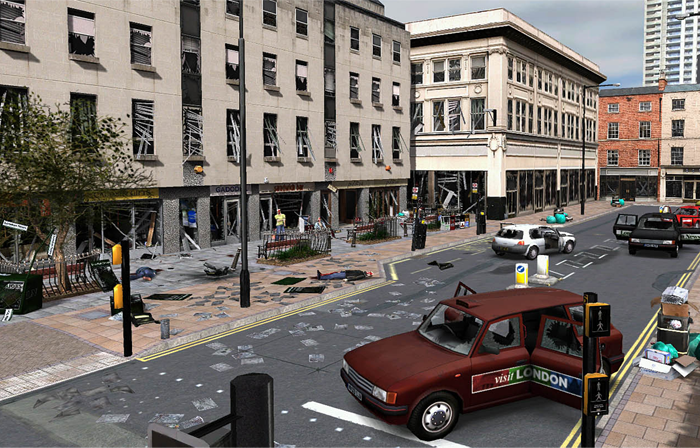
\includegraphics[scale=0.5]{tics/images/triage.png}
\caption{Ambientación de Triage}
\label{fig:triage}
\end{figure}

\emph{Triage Trainer} se desarrolla en una escena de explosión en una calle
(ver~\ref{fig:triage}) la cual es un incidente mayor, y está diseñado para
formar profesionales que puedan participar en una escena de un incidente de este
tipo (médicos, enfermeros, paramédicos, rescatistas). Los jugadores deben
realizar un triage, es decir, evaluar el grado de las lesiones de víctima, las
cuales son generadas aleatoriamente, utilizando los protocolos y controles
médicos adecuados, además de priorizar a las víctimas para el tratamiento. La
apariencia física de cada víctima es imitada con precisión como los signos
vitales, los síntomas y sobre todo los patrones de tiempo para el deterioro de
las lesiones, es decir, la condición de una víctima cambia de forma realista con
el tiempo (ver~\ref{fig:triage_patient1}).

\begin{figure}[h!t]
\centering 
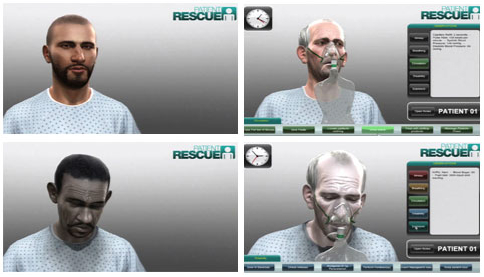
\includegraphics[scale=0.5]{tics/images/patient_side.jpg}
\caption{Evolución de un paciente en Triage}
\label{fig:triage_patient1}
\end{figure}

Al finalizar cada simulación los jugadores reciben retroalimentación acerca de
su rendimiento, incluyendo la precisión de sus chequeos, si los pacientes fueron
priorizados en el orden correcto y el tiempo que les llevó completar el triage,
en comparación con la de un experto.

La retroalimentación de los participantes que utilizaron Triage Trainer sugiere
que el mismo cumplió exitosamente sus fines. Los jugadores asociaron su
experiencia de juego con su experiencia en el mundo real y muchos de ellos
sentían que realmente estaban allí. Se espera que los jugadores puedan tomar
decisiones bajo presión, lo que ayudará a su desarrollo cognitivo. También se
observó que los jugadores tienden a discutir sus experiencias con sus compañeros
de curso, lo que también podría tener un impacto en su aprendizaje.

Un elemento que no fue evaluado por \emph{TruSim} debido a que no era
logísticamente posible fue el impacto de las pruebas en la retención del
conocimiento y el cambio de comportamiento de los
jugadores\cite{education:games}. 


\subsection{Caso 2 SimVenture}

\begin{description}
\item[Tipo:] Juego de simulación de negocios.
\item[Destinatarios:] Personas de 14 a 30 años.
\item[Contenido:] Las realidades de la creación y funcionamiento de un negocio.
\item[Desarrollador:] \emph{Venture Simulations.}
\end{description}

En el inicio del juego (ver~\ref{fig:simventure_tutorial}), a los jugadores se
les brinda informaciones y antecedentes para que que se ubiquen en escena. Ellos
deben empezar a dirigir su propio negocio en su casa de fabricación y venta de
computadoras, mientras deben mantener un trabajo de tiempo completo
independiente. El juego lleva a los jugadores a la ejecución de un negocio en su
propia casa y a la extensión del mismo a más locales, lo que requiere
contratación de personal. Los jugadores son capaces de avanzar en el juego a
través del aprendizaje de los elementos importantes de la empresa, organizadas
en cuatro categorías: organización, ventas/marketing, finanzas y operaciones.
Los jugadores toman decisiones acerca de las actividades dentro de estas áreas y
observan los resultados de sus acciones. 

\begin{figure}[h!]
\centering 
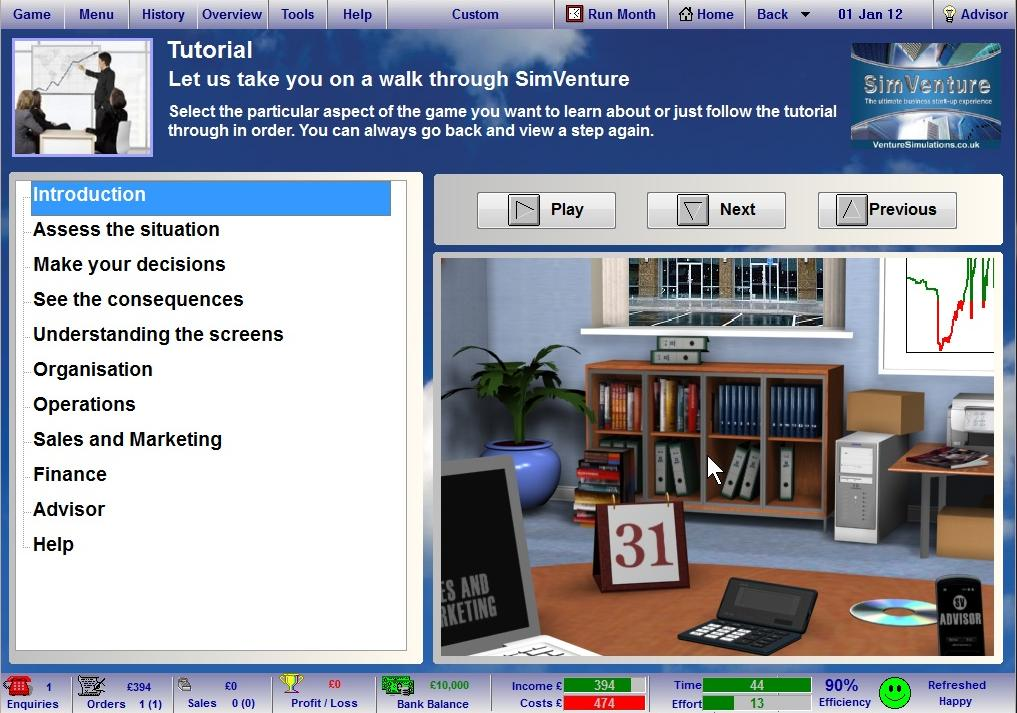
\includegraphics[scale=0.5]{tics/images/simventure-tutorial.jpg}
\caption{Tutorial de SimVenture}
\label{fig:simventure_tutorial}
\end{figure}

Los jugadores obtienen retroalimentación sobre un número de diferentes
parámetros. En un nivel básico, se puede simplemente revisar la cantidad de
ingresos que están generando. Además de esto, el éxito puede ser medido por la
cantidad de pedidos que han recibido para sus productos. También se proporciona
retroalimentación visual para representar la eficiencia de la organización y su
felicidad como individuo.

\emph{Phil Warren}, director de estudios de negocios en \emph{Snaith School}, ha
utilizado \emph{SimVenture} como complemento al plan de estudios. Según el
mismo, el plan de estudios por lo general sólo requiere que los estudiantes
aprendan sobre los diversos elementos del negocio de forma aislada, sin embargo
en la realidad, cualquier decisión que se tome en una de las partes de un
negocio tiene efecto en las demás. \emph{SimVenture} se vio como una oportunidad
de aplicar los conocimientos aprendidos en clase en una actividad práctica,
además se observó que permitir que los estudiantes jueguen en pares da un
espacio para la discusión en torno a las decisiones y aprenden de sus errores
juntos\cite{education:games}.


%! TEX root = ../main.tex
\chapter{Propuesta de solución}
\label{chap:solucion}

%%! TEX root = ../main.tex


\section{Acciones condicionadas por eventos}

Un evento es la ocurrencia de un hecho en particular, y son identificados por un
nombre y un conjunto de parámetros, por ejemplo, cuando un evento es cuando el
enfermero inserta una Jeringa, el nombre de este evento es
\emph{''jeringa.inserted''}, y sus parámetros podrían ser el lugar y el tiempo
de la inserción, así, la influencia del estudiante en la simulación es una
sucesión de eventos.

Por cada acción que realiza el usuario dentro de la simulación, existe un evento
relacionado, por consiguiente, es razonable estudiar algunos eventos para
determinar si los pasos realizados corresponden con los deseados. 

Para determinar si una sucesión de eventos es la correcta, se definen reglas,
una regla es una asociación de una condición y una acción, la condición define
si el entorno es el adecuado para realizar una acción, la cual es un
procedimiento que realiza la lógica deseada.

Las \gls{eca} son aquellas que son activadas una vez que se cumplen determinados
eventos\cite{bailey2004event}. En las bases de datos relacionales, son conocidos
como triggers, es decir, una base de datos relacional (u orientada a objetos) es
un motor de reglas \gls{eca}\cite{bailey2004event}\cite{behrends2006combining}.

Las mismas pueden ser utilizadas para notificar que un determinado conjunto de
eventos ha ocurrido\cite{bailey2004event}, así como servir para almacenar
información acerca de la utilización de un determinado recurso.


\subsubsection{Motivación}

Las reglas del tipo \gls{eca} permiten reaccionar a determinados eventos, en
forma de una única regla, la cual facilita la declaración de las
mismas\cite{bailey2004event}.

Son principalmente útiles para analizar el comportamiento en tiempo real de un
sistema en una forma
reactiva\cite{bailey2004event}\cite{de2001eca}\cite{bailey2002analysis}, esta
característica esta impulsada principalmente por que son ejecutadas después de
la ocurrencia de un evento, y el entorno no es modificado, pudiendo así acceder
al mismo entorno que el qué lanzo el evento.

Definir si las acciones de un usuario son correctas utilizando un motor
\gls{eca} es sencillo desde el punto de vista que sólo se deben definir un
conjunto de acciones que se deben realizar, y agregar una acción que verifica si
los pasos realizados fueron los correctos.

\subsection{Declaración}

Una \gls{eca}, se define como\cite{bailey2004event}\cite{behrends2006combining}:

\begin{center}
	 Cuando ocurren una serie de \emph{eventos}, y se cumple una
	 \emph{condición}, entonces realizar una \emph{Acción}.
\end{center}

Los \emph{eventos} determinan cuando una regla debe ser activada, los mismos se
dividen en dos categorías\cite{behrends2006combining}, primitivos y compuestos,
los primeros son detectables, por ejemplo, cuando se inserta una jeringa, y los
compuestos, son la combinación de uno o más
primitivos\cite{bailey2004event}\cite{behrends2006combining}. Los eventos
compuestos, se unen mediante:
\begin{enumerate*}[label=\itshape\alph*\upshape)]
\item conjunción (\emph{y}),
\item disyunción (\emph{o}), y
\item secuencia (\emph{entonces}).
\end{enumerate*}
Sin embargo, no siempre son necesarios todas las posibles combinaciones, y las
combinaciones sencillas son más fáciles de optimizar y
probar\cite{bailey2004event}.

La \emph{condición} de una regla determina si el entorno es el necesario para que la
regla sea activada, en esta condición el entorno que lanzó el evento esta
disponible.

La \emph{acción} a ejecutar describe la lógica que debe ser ejecutada cuando se han
lanzado los eventos y la condición de la regla se ha cumplido.

\subsubsection{Dependencia entre reglas}

Las reglas pueden depender de otras reglas, lo cual se puede ver como que la
finalización de una regla es un evento que otra regla espera para poder ser
activada.

Las reglas pueden agregar información a un contexto compartido por todas las
reglas, de esta manera, se puede pasar parámetros entre distintas reglas, por
ejemplo, la regla \emph{Retirar Torniquete}, depende de la regla \emph{Insertar
Torniquete}, pero debe responder solamente al torniquete que ha activado
la regla de inserción, es decir, el usuario puede extraer varios torniquetes, y
la regla no debe activarse, hasta que se extraiga el torniquete que activo la
primer regla.

Así, la regla \emph{Retirar Torniquete} depende de la regla \emph{Insertar
Torniquete}, y esta relación entre reglas, se da en dos
formas\cite{bailey2004event}:

\begin{itemize}
\item  \emph{Dependencia fuerte:} la regla \emph{Retirar Torniquete} solamente podrá
	ser elegida para ser lanzada cuando la regla \emph{Insertar Torniquete}
	haya sido cumplida.
\item  \emph{Dependencia de contexto}: la regla \emph{Retirar Torniquete} no se
	activará cuando los eventos a los que escucha se terminen, sino cuando
	los eventos a los que escucha sean lanzados con los parámetros adecuados
	(se extraiga el torniquete que lanzo la regla de inserción).
\end{itemize}

\subsubsection{Definición}

La definición de las reglas se realiza de la siguiente forma;
\begin{algorithm}[H]
\caption{Creación de regla de verificación de calzado de guantes}
\label{alg:rule:guante}
\lstset{style=sharpc}
\begin{lstlisting}
Rule.New("Regla de verificacion de calzado de guantes").
     When("enfermero.guantes.calzar").
     Then(e => e.Patient.ManosLimpias()).
\end{lstlisting}
\end{algorithm}
%TODO agregar indice de algoritmos

La regla anterior controla que el estudiante ha realizado la acción ``Calzarse
los guantes'', y en ese momento tenga las manos limpias, la variable \emph{e},
es el entorno, y a través de la propiedad \emph{Patient} obtiene el estado del
paciente en ese momento.

\subsection{Modelo de ejecución}

Para ejecutar un motor de reglas del tipo \gls{eca}, se debe tener en cuenta
principalmente dos factores, 
\begin{enumerate*}[label=\itshape\alph*\upshape)]
\item  Como se verifica el cumplimiento de cada regla, y, 
\item  Que ocurre cuando varias reglas son lanzadas al mismo tiempo
\end{enumerate*}.

Para ambos casos se puede tomar un enfoque \emph{inmediato}, es decir que
inmediatamente cuando se lanza un evento, o se cumple una condición, se ejecuta
la regla. Además existen otros dos modos de ejecución, \emph{deferida}, y
\emph{desacoplada}, en la primera, se espera hasta que el lanzador del evento
culmine su trabajo, y luego se ejecuta la regla, pero en la misma unidad de
trabajo, mientras que en la ejecución desacoplada, se encolan los trabajos y
otro hilo es el encargado de ejecutar las reglas. Estos modos están inspirados
en las bases de datos relacionales, el deferido se ejecuta en la misma
transacción, y el desacoplado, inmediatamente después de que la transacción
termine\cite{bailey2004event}.

La propuesta implementada, utiliza una ejecución inmediata, principalmente por
la sencillez de las reglas, es decir, las reglas no realizar un proceso complejo,
solamente controlan el estado del entorno y lo validan.

Además, la ejecución inmediata es importante por que el entorno no sufre
modificaciones entre el evento lanzado y la ejecución de la regla, según
\cite{bailey2004event}, este es el factor más importante para determinar el tipo
de ejecución deseado.



\subsubsection{Estados de una regla}

Una regla puede estar en uno de los siguientes estados:

\begin{description}
\item[BEGIN] Es una regla que recién fue creada, no realiza ninguna
	acción.
\item[WAITING\_FOR\_RULE] Es un estado en el que esta esperando que otras reglas
	sean lanzadas. En este estado, es un suscriptor de las reglas por la que
	espera, y no forma parte del ciclo de ejecución del motor de reglas.
\item[WAITING\_FOR\_EVENT] Es un estado en el que esta escuchando a que sean
	lanzados los eventos a los que escucha, este es el estado principal. En
	este estado, es un suscriptor de los eventos por los que espera, y no
	forma parte del ciclo de ejecución del motor de reglas. Se diferencia
	del estado anterior, en que los eventos escuchados pueden ser lanzados
	por cualquier objeto del entorno, no necesariamente una regla.
\item[WAITING\_FOR\_CONDITION] La regla ya no espera por ningún evento y las
	reglas de las que depende ya han sido lanzadas, se verifica cada cierto
	tiempo si el entorno cumple con una condición definida. 
\item[FINISH] La regla ha sido lanzada, con un resultado no determinado, se pudo
	haber cumplido, como no, es el estado final de una regla. Cuando una
	regla llega a este estado, se lanza su evento de finalización.
\end{description}

Una regla puede estar en solo un estado, y solamente se permite que el estado
avance, desde \emph{BEGIN} hasta \emph{FINISH}.


\subsubsection{Ciclo de vida}

Cuando una regla es definida, y insertada al motor de reglas, inmediatamente
pasa al estado \emph{BEGIN}, luego se verifica si la misma depende de otras
reglas, sí este es el caso, pasa al estado \emph{WAITING\_FOR\_RULE} y escucha a
los eventos de finalización de las reglas anteriores.

Una vez que las reglas anteriores han sido finalizadas, la regla pasa al estado
\emph{WAITING\_FOR\_EVENT} sí deben escuchar por algún evento, en caso contrario
pasan al estado \emph{WAITING\_FOR\_CONDITION}.

Una vez que la regla está en estado \emph{WAITING\_FOR\_CONDITION}, pasa a un
motor que ejecuta su condición cada cierto tiempo, si la condición se cumple, la
regla se ejecuta, y la misma pasa a estado \emph{FINISH}, momento en el cual
notifica a las reglas que dependen de ella que ha sido lanzada.

Una vez que la regla esta en estado \emph{FINISH}, la misma sale del esquema de
ejecución, y solo esta disponible para obtener resultados.

Según el ejemplo de la regla definida en el código \ref{alg:rule:guante}, la
regla al terminar de ser construida pasa a estado \emph{BEGIN}, al no depender
de otras reglas, pasa inmediatamente al estado \emph{WAITING\_FOR\_EVENT},
cuando es lanzado el evento, la regla ejecuta la acción y pasa al estado
\emph{FINISH}.

\subsubsection{Motor de ejecución}

Un motor de reglas \gls{eca}, requiere de un proceso que evalúe constantemente
las reglas para verificar si las mismas deben ser lanzadas o
no\cite{bailey2004event}\cite{galton2002two}, este motor puede utilizar el
algoritmo de RETE\cite{de2001eca} para realizar esta verificación, en la
propuesta presentada, la cantidad de reglas definidas, y la no dependencia
circular entre ellas, hace innecesario la implementación de tal
algoritmo\cite{de2001eca}. 

El motor de reglas actúa sobre aquellas reglas en estado
\emph{WAITING\_FOR\_CONDITION} e invoca al procedimiento que se encarga de
validar si la regla puede ser activada (el procedimiento es único por cada
regla), si el mismo determina que la regla puede ser lanzada, el motor ejecuta
la acción de la regla y modifica el estado de la regla a \emph{FINISH}.

\section{Descripción general de la solución}

Una vez descriptos los fundamentos teóricos del uso de videojuegos en el ambiente educativo sobre todo en aquellos que requieren de mucha practica para plasmar los conocimientos. Siendo el área de enfermería una de estas áreas definimos las problemáticas actuales de esta y seleccionamos algunos procedimientos que serán utilizados para el contenido de la solución. A continuación se busca converger todos los aspectos descriptos en
capítulos anteriores.

La solución propuesta en este trabajo consiste en el desarrollo de una aplicación para dispositivos móviles que se define como un juego serio llamado YAVE el cual incluye ciertos aspectos de gamification. El juego consiste en ofrecer a los usuarios, en este caso alumnos de enfermería, un medio en el cual puedan realizar procedimientos de enfermería y el cual les puede servir como herramienta de apoyo en su aprendizaje.

YAVE permitirá al usuario poder seleccionar el procedimiento que quiera realizar, en cada procedimiento se le dará la posibilidad de interactuar con un paciente y con una conjunto de objetos que forman parte de las herramientas requeridas para realizar el procedimiento en cuestión. Además, le permitirá realizar acciones de bioseguridad.

La aplicación no solo le permitirá al usuario realizar los procedimientos para poner en practica sus conocimientos sobre el mismo sino también evaluará al usuario, dándole al final de la partida una puntuación final y diciéndole cuales son los pasos que realizó de manera correcta y cuales de manera incorrecta, proporcionándole una pequeña información sobre su error.
%! TEX root = ../main.tex
\section{Tecnologías disponibles}

Para el desarrollo de videojuegos se utilizan programas o herramientas
especializadas en ello llamadas \enquote{Motores de videojuegos}. A continuación
se da una breve introducción de lo que es un motor de videojuego o motor
gráfico.

El término \enquote{motor gráfico} o \enquote{motor de videojuegos} hace
referencia a una serie de rutinas de programación que permiten el diseño, la
creación, el desarrollo y la representación gráfica de un
videojuego\cite{videojuego:telechea}.

Además, la gran mayoría de estos motores ofrecen a su vez características y
funciones que facilitan la construcción del videojuego, como el motor físico
(software capaz de realizar \enquote{simulaciones} de ciertos sistemas físicos
como la dinámica de un cuerpo rígido, el movimiento de un fluido o la
elasticidad) o detector de colisiones, sonidos, \textit{scripting}, animaciones,
inteligencia artificial, comunicación a través de redes, \textit{streaming},
administración de memoria, etc\cite{videojuego:telechea}.

El motor de juego utilizado depende de las características que posea el
videojuego que se quiere desarrollar. Por lo mismo, a continuación se da una
breve descripción de los motores más utilizados actualmente, se definen los
criterios para de selección y se realiza una comparación entre los mismos, y se
define el motor que más se adecue a las necesidades.

\subsection{Unreal Development Kit}

\textit{Unreal Engine} es el motor de juegos desarrollado por \textit{Epic
    Games}, se ofrece bajo un plan de suscripción mensual. El servicio de
suscripción permite a los desarrolladores unirse a una comunidad dedicada a la
construcción de grandes juegos y evolución del \textit{Unreal
    Engine}\cite{unrealengine}.

\textit{Unreal Engine} permite desarrollar juegos para plataformas como
\textit{Windows PC, Mac, iOS y Android}. También es compatible con \textit{Xbox
    One} y \textit{PlayStation 4}. Existen además trabajos recientes sobre otras
plataformas como \textit{HTLM5} y \textit{Linux}\cite{unrealengine}.

Sin embargo existe una versión gratuita del \textit{Unreal Engine}, el
\Gls{udk}. El \Gls{udk} es la edición gratuita de \textit{Unreal Engine
    3}\footnote{Versión previa a la actual versión comercial.} que proporciona
acceso al motor de juegos 3D y a la herramienta profesional que se utiliza en el
desarrollo de videojuegos \textit{blockbuster}, visualización arquitectónica, el
desarrollo de juegos para móviles, modelos 3D, películas digitales y más.
Utilizando \Gls{udk} se pueden implementar juegos y aplicaciones en
\textit{Windows PC}, \textit{iOS} y \textit{Mac}.


\subsection{Blender Game Engine}

\enquote{Blender Game Engine} es el motor de juego de \textit{Blender
    Foundation} que permite crear aplicaciones 3D interactivas o simulaciones,
desarrollabo bajo la licencia \Gls{gnu}. La principal diferencia entre el
\textit{Blender Game Engine} y el Blender convencional está en el proceso de
renderizado\cite{blender}.

Es importante no confuir con \textit{Blender}, pues este es un software de
modelado \textit{3D} y animaciones, pero esto se renderiza fuera de linea, es
decir, una vez generadas no pueden ser modificadas. Por el contrario
\textit{Blender Game Engine} genera las escenas de forma continua en tiempo real
e incorpora facilidades para la interacción del usuario durante el proceso de
\textit{renderización}\cite{blender}.

Procesa la lógica de sonido, de la física y la representación de simulaciones en
orden secuencial. El motor esta escrito en \textit{C++}. Posee un editor que
proporciona una profunda interacción con la simulación, su funcionalidad se
puede ampliar con \textit{scripts} \textit{Python} y esta diseñado para abstraer
las características complejas del motor en una interfaz de usuario simple, que
no requiere programación\cite{blender}.

El motor de juego puede simular contenido dentro de \textit{Blender}, sin
embargo, también incluye la posibilidad de exportar en plataformas como
\textit{Windows, Linux y Mac OS}. También hay soporte básico para plataformas
móviles con el proyecto \textit{Android Blender Player GSOC 2012}.

\subsection{CryEngine 3}

\enquote{CryEngine 3} es el motor de juegos desarrollado por \textit{Crytek}.
\textit{CryEngine} es un motor avanzado para el desarrollo de juegos, películas,
simulaciones de alta calidad y aplicaciones interactivas. Tiene características
diseñadas específicamente para \textit{Windows PC, PlayStation 3 y Xbox
    360}\cite{cryengine}.

Existe una versión gratuita de \textit{CryEngine}, denominada \enquote{CryEngine
    Free SDK} con todas las funcionalidades, esta versión esta disponible para
su descarga, pero ya ha sido descontinuada\cite{cryengine:sdk}.

\textit{CryEngine} posee además un conjunto de herramientas utilizadas para el
análisis de rendimiento\cite{cryengine}, además de un \Gls{ide}, que permite
editar texturas, interacciones, vehículos, etc.

\subsection{ShiVa3D}

\textit{ShiVa3D} es un paquete para el desarrollo de juegos y aplicaciones 3D,
posee un \Gls{ide} \Gls{wysiwyg} potente\cite{shiva}.

\textit{ShiVa} puede exportar juegos y aplicaciones para más de $20$ plataformas
de destino, incluyendo móviles como \textit{iOS, Android, BlackBerry y Windows
    Phone}, de escritorio como \textit{Windows, Mac OS X y Linux}, los
navegadores web con soporte \textit{Flash y HTML5}, así como consolas como la
\textit{Xbox 360, PlayStation3 y Nintendo Wii}. El \Gls{ide} se ejecuta en
\textit{Windows} y \textit{Mac OS X}\cite{shiva}. 

Un producto relacionado es el \enquote{ShiVa Server}, el cual permite el
desarrollo de aplicaciones multijugador. Las carácteristicas de este servidor,
incluyen alto rendimiento, comunicación \textit{VoIp}, etc. \enquote{ShiVa
    Server} se distribuye con una licencia distinta a
\textit{Shiva3D}\cite{shiva}.

\subsection{Unity3D}

\textit{Unity}\cite{unity3d} es un motor para el desarrollo de juegos,
dearrollado por \textit{Unity Technologies}, incluye un \Gls{ide} con un un
motor de \textit{renderizado} y flujos de trabajo para la creación de contenido
3D interactivo, desarrollo multiplataforma. Además cuenta con una gran cantidad
de \textit{assets}\footnote{Un \textit{Asset} es un paquete \textit{Unity} que
    puede contener modelos, librerias, sonidos, etc.} disponibles en un
\enquote{Asset Store} y una gran comunidad donde se intercambian conocimientos.

En \textit{Unity} se pueden desarrollar de forma sencilla elementos 2D y 3D.
Posee un \Gls{ide} intuitivo y flexible, el nivel visual y de audio son de gran
calidad, un sistema de animación poderoso. 

Permite desarrollar juegos para múltiples plataformas. Entre las plataformas
móviles soportadas, encontramos a \textit{iOS, Andriod, Windows Phone 8,
    BlackBerry 10}, entre las plataformas de escritorio a \textit{Windows, Mac y
    Linux}, plataformas web como \textit{Internet Explorer, Mozzilla Firefox,
    Google Chrome}\footnote{Requiere un plugin para el navegador que está
    disponible para \textit{Windows y Mac}}, y entre plataformas de consolas a
\textit{Xbox 360, Xbox One, Wii, Wii U, Nintendo 3DS}.

La versión paga de \textit{Unity}, \textit{Unity Pro} permite además plataformas
como \textit{PlayStation 4, PlayStation 3 y PlayStation VITA}.

Debido a la alta popularidad de \textit{Unity}, un paquete fue desarrollado por
\textit{Facebook} que permite una interacción sencilla con la \Gls{api} de la
red social \textit{Facebook} en un \textit{Asset} escrito en \cs{}, este paquete
se encuentra en \textit{Asset Store} de \textit{Unity}.

\section{Selección de plataforma}
\section{Hipótesis de la simulación}
\label{sec:hipotesis}


\observacion{Ver en la tésis de Tardon: \emph{no es necesario simular todos los
        pasos}.}

Las escenas seleccionadas y definidas en~\ref{sec:seleccion_escenas} representan
las acciones que deben realizar los profesionales de enfermería a la hora de
realizar los procedimientos seleccionados, por limitaciones técnicas,
tecnológicas y de tiempo, no es posible realizar una simulación de todos los
pasos requeridos.

Los factores que influyen en que partes se simularán, que partes estarán
presentes solamente a través de opciones y que partes se omitirán son:

\begin{itemize}

    \item \textbf{Limitaciones técnicas}: acciones como la simulación del agua
        (necesarios para el lavado de manos), requieren de requisitos de
        hardware avanzados y un tiempo considerable de desarrollo. Las acciones
        que escapan al alcance del hardware y tiempo de los desarrolladores no
        son simuladas.

    \item \textbf{Importancia}: no todos los pasos definidos en el procedimiento
        oficial son necesarios, por ejemplo, la colocación de los elementos
        cerca del lugar de trabajo, es un paso necesario, pero es considerado un
        paso poco importante y trivial.

        La importancia es evaluada por profesionales del \Gls{iab}, los cuales
        dieron su opinión acerca de cada aspecto simulado, el mismo es tenido en
        cuenta para determinar la importancia de cada acción.

    \item \textbf{Facilidad de realización en la vida real o en el laboratorio}:
        ciertos pasos son triviales en la vida real pero requieren un esfuerzo
        significativo para ser simuladas, como por ejemplo el lavado de manos es
        un procedimiento al que los alumnos están acostumbrados.

        La facilidad que tienen los alumnos con las acciones fue determinada por
        profesores del \Gls{iab}, determinaron que acciones son triviales para
        los alumnos y cuales presentan mayores dificultades en su vida
        profesional.

        Otro aspecto que influye en la facilidad de realización de los
        procedimientos es la familiarización, si los alumnos están
        familiarizados con los procedimientos, estos no son simulados.

\end{itemize}

Estas hipótesis sirven para acotar el alcance de la simulación, definen qué se
simulará y cual es del detalle necesario para alcanzar las competencias básicas.

Existen hipótesis que son globales para toda la simulación, las mismas son:

\begin{itemize}

    \item \textbf{Comandos de voz con interfaz}: para enviar una petición al
        paciente (por ejemplo, preguntarle su nombre), no es necesario
        identificar las palabras del usuario, sino más bien detectar que ha
        hablado y listar las posibles acciones que se pueden realizar.

    \item \textbf{Utilización de la interfaz}: para realizar una acción con los
        elementos, es suficiente con presionar el mismo y seleccionar una acción
        de una lista de opciones, no hace falta emular todas las posibles.

    \item \textbf{Acciones de bioseguridad}:\todox{Definir bioseguridad} Las
        acciones de bioseguridad, se realizan a través de una opción en la
        interfaz gráfica.

\end{itemize}

Otras hipótesis, son tomadas por escena, las dos escenas simuladas son
diferentes en el modo de interacción del usuario con su entorno, por ejemplo, en
la escena de extracción de sangre, el usuario interactúa con el paciente a
través de objetos, en la evaluación de Glasgow, la interacción con el paciente
es directa.

\subsection{Extracción de sangre}

Se presentan los pasos mostrados en la sección~\ref{sec:hemocultivo_protocolo},
y adicionalmente se establecen las hipótesis punto por punto y las
consideraciones que deben ser tomadas.

\begin{itemize}

\item \textbf{Preparar el equipo}: la preparación del equipo es un aspecto muy
    importante del procedimiento, pero no es un punto único de la extracción de
    sangre, además las prácticas de los alumnos cubren completamente este paso
    según comentarios de los profesores. \emph{Este paso no se simula}.

\item \textbf{Explicación al paciente del procedimiento a realizar}: es un
    aspecto importante del procedimiento, pero la simulación de una conversación
    alumno-paciente es compleja, según comentarios de los profesores, es
    suficiente con que los alumnos sepan que lo deben realizar y en que moento,
    no es necesario simular la conversación en sí. \emph{Este paso se simula a
        través de un comando de voz con la interfaz}.

\item \textbf{Asepsia de las manos}: este paso forma parte de un área más amplia
    conocida como bioseguridad, la cual es un aspecto transversal a todos los
    procedimientos realizados por los enfermeros. 
    La implementación de una simulación del lavado de mano es compleja, y es un
    aspecto que, al igual que la preparación del equipo, está cubierta por los
    laboratorios, aún así, es necesario que los alumnos sepan en que momento
    deben realizar la asepsia de sus manos. \emph{Se simula este paso a través de una
        opción en la interfaz}, no se simulan los pormenores del lavado de manos.

\item \textbf{Llevar el equipo a la unidad en donde se encuentra el paciente}:
    este es un paso trivial que deben realizar los profesionales, la simulación
    de este proceso no es importante según comentarios de los profesores. Este
    proceso no tiene importancia según los profesionales del \Gls{iab}, \emph{este
        paso no se simula}.

\item \textbf{Vestirse con bata estéril, tapaboca y gorro}: al igual que la
    asepsia de las manos, es importante que los alumnos sepan que lo deben
    hacer, pero no es importante que se simule como lo hacen. 

    Los estudiantes están familiarizados con estas acciones, \emph{se simula el
        momento y el orden en el que el jugador lo hace} a través de una opción
    en la interfaz, no se simula el proceso en sí.

\item \textbf{Calzarse los guantes}: es un paso relacionado a la bioseguridad,
    es importante que se sepa en que momento debe realizarse, pero no es
    necesario simular el proceso. 
    \emph{Se simula el momento y el orden en el que se realiza}, no se simulan
    los pormenores de la acción.

\item \textbf{Ubicar al paciente en posición adecuada}: la ubicación del
    paciente durante la extracción de sangre es un factor determinante para que
    la extracción pueda ser realizada correctamente.

    Los alumnos están familiarizados con este proceso según opinion de los
    profesionales, \emph{este paso no se simula}, el paciente está en la
    posición adecuada al inicio de la simulación.

\item \textbf{Elegir la zona a puncionar}: existen varias partes del antebrazo
    donde se puede proceder a realizar una inyección, el conocimiento de las
    mismas, y el procedimiento para detectarlas, es un factor importante del
    proceso.
    
    Las venas del cuerpo humano se detectan palpando los antebrazos, y sintiendo
    el pulso del paciente, existen dos áreas donde el pulso es suficientemente
    fuerte como para sel palpado, estos puntos y el pulso del paciente deben ser
    detectables por el jugador.

    \emph{Los puntos donde se debe punzar deben son identificables en la
        simulación}, a través de una palpación a los brazos del paciente. 

\item \textbf{Colocación del torniquete}: La ubicación y el momento de la
    colocación del torniquete es de vital importancia para el procedimiento, el
    mecanismo utilizado para colocarlo no es relevante, pues el mismo es
    trivial.

    \emph{El hecho de colocar el torniquete es simulado}, el mecanismo para
    hacerlo no es importante.

\item \textbf{Solicitar al paciente que cierre el puño}: El momento en el cual
    se solicita al paciente que cierre la mano es vital para que el
    procedimiento de extracción sea satisfactorio.

    \emph{Este paso es simulado} a través de un comando de voz.

\item \textbf{Esterilizar la zona de punción}: la esterilización de la zona de
    punción es un factor de suma importancia para el procedimiento, así como el
    momento en el que se realiza, \emph{el jugador debería poder esterilizar} la
    zona antes de insertar la jeringa.
    
\item \textbf{Extraer el protector de la aguja}: La extracción del protector de
    la aguja es un paso necesario, pero trivial, el hecho de retirar el
    protector de la jeringa \emph{no es un paso necesario para el logro de las
        competencias básicas necesarias}, por ello, no se simula.

\item \textbf{Puncionar la piel con la aguja}: este es un paso central en el
    procedimiento, en el se deben tener en cuenta aspectos como la posición
    donde se realiza la punción, y el angulo con el que ingresa la aguja.

    La posición donde se realiza la punción es importante por que depende de la
    ubicación donde se colocó el torniquete, y debe ser en uno de los puntos del
    brazo donde existen venas capaces de soportar el procedimiento, \emph{en
        cada brazo existen dos puntos donde se puede inyectar}.

    En cuanto al ángulo de punción, es un conocimiento importante que deben
    tener los alumnos, el conocimiento es teórico y según comentarios de los
    profesores, es un tema en el cual los alumnos tienen suficiente práctica en
    el laboratorio, \emph{No se simula el ángulo en el cual se inserta la
        jeringa}, es decir, la jeringa siempre se inserta en el mismo angulo.

\item \textbf{Tensar la zona de punción}: el proceso de tensar la zona de
    punción se realiza momentos durante la inserción de la jeringa, el mismo es
    trivial, y para simularlo se requiere que el usuario utilice tres dedos al
    mismo tiempo (dos para tensar y otro para realizar la punción), lo cual
    dificulta la utilización de la solución.

    \emph{Este paso no se simula} por la dificultad técnica que implica utilizar
    tres dedos para realizar una tarea, conjuntamente con la facilidad con que
    se realiza acción. 

\item \textbf{Remover el torniquete}: Al igual que en la colocación del
    torniquete, \emph{se simula el momento} de la extracción por que es
    importante, pero no los detalles de la extracción.

\item \textbf{Solicitar la apertura del puño}: el momento exacto donde se debe
    solicitar al paciente que abra la mano es fundamental para la realización
    correcta de la simulación. \emph{Este paso se simula} a través de un comando
    de voz.

\item \textbf{Extraer la muestra se sangre necesaria}: este es el paso central
    de la práctica, tanto el momento, como la forma es importante simular.

    La extracción de la sangre \emph{se simula} la acción de la extracción, pero
    no detalles como la sangre extraída, la velocidad de extracción y la fuerza
    necesaria por limitaciones de la tecnología.

\item \textbf{Presionar el brazo y extraer la aguja}: la presión del brazo para
    extraer la jeringa es un paso trivial, en cambio el momento en el que se
    extrae la aguja es conocimiento necesario para el procedimiento.

    \emph{No se simula esta acción}, pues es un paso al que los alumnos están
    acostumbrados y de simularse, agrega una complejidad adicional a la
    extracción, que es un paso que se realiza al mismo tiempo.

\item \textbf{Colocar algodón con alcohol en el punto de punción}: este paso es
    importante, tanto el momento en el cual se debe realizar, como la forma de
    realizarlo.

    \emph{Se simula la colocación del algodón}, así como el tiempo que se debe
    presionar el mismo.

\item \textbf{Sellar la muestra y enviarlo a su destinatario}: es necesario que
    los alumnos sepan que este paso debe ser realizado, pero los detalles del
    mismo, no son necesarios para el logro de las competencias básicas,
    \emph{este paso no se simula}.


\item \textbf{Retirar la bata, tapaboca, gorro y guantes}: es necesario que los
    alumnos sepan que deben desechar todos los elementos que fueron utilizados
    durante el proceso, la forma de hacerlo no es necesaria.

    \emph{Se simula el momento en el que se extraen los elementos} a través de
    una opción en la interfaz.

\item \textbf{Asepsia de las manos}: la asepsia final de las manos es un paso
    necesario para el procedimiento, así como la asepsia inicial, es importante
    que los alumnos sepan el momento en cual deben realizarlo, \emph{este paso
        se simula} a través de una opción en la interfaz.

\end{itemize}

Estas hipótesis afectan directamente el desarrollo de la aplicación, dictando
que partes del procedimiento se simulan y como, pueden ser vistas como
requisitos funcionales de la solución.

\subsection{Evaluación de glasgow}

En la sección~\ref{sec:glasgow_protocolo} se definieron los pasos necesarios
para poder llevar a cabo el procedimiento, este procedimiento es un paso
rutinario que deben realizar los profesionales para poder determinar rápidamente
el estado de conciencia de un individuo. 

El paso central de la práctica es la valoración del paciente y la generación del
diagnostico, los demás pasos, no colaborar en el desarrollo de la competencia
básica y según opiniones de los profesores no son importantes.

Así, es suficiente con simular al paciente y las reacciones que tiene ante las
acciones del jugador, y las siguientes hipótesis se basan en la interacción
paciente/jugador.

El último paso del procedimiento es el registro final de la puntuación, el mismo
es utilizado como mecanismo de evaluación y el registro en sí no se simula, es
decir, se solicita al jugador que realice el diagnostico (mediante un menú),
pero no en la condiciones que se utilizan en la vida real (anotando en el
registro médico del paciente).

Para simular la medición del estado del paciente, se toman las siguientes
hipótesis:

\begin{itemize}
    \item La provocación de un estimulo doloroso al paciente es una accion
        necesaria, pero no así los detalles de la misma, \emph{se simula el
            estimulo con una opción} al personar al paciente en alguna
        extremidad.
    \item El dialogo jugador/paciente se realiza a través de comandos de voz, el
        nombre del paciente es una información que se conoce de ante mano y
        \emph{Se simulan 7 posibles preguntas}, que incluyen solicitudes de
        apertura ocular, movimiento de extremidades, y preguntas generales como
        el nombre del paciente, el día y el lugar.
\end{itemize}



%! TEX root = ../main.tex

\section{Solución}
\label{sec:solucion}

A continuación se describe la arquitectura propuesta para la realización de una juego serio, se
utiliza la guía básica definida por~\cite{pereira2009design} y descrita
en~\ref{sec:desarrollo}.

Esta sección se enfoca en los aspectos técnicos de la creación del juego serio,
las competencias básicas relacionadas con la educación (segundo paso de la guía
descrita en~\ref{sec:desarrollo}) se definieron en las
secciones~\ref{sec:glasgow} y~\ref{sec:hemocultivo}.

\subsection{Partes de la simulación}

La simulación se compone de tres elementos principales, entidades (que son
objetos de la vida real), acciones (que son provocadas por las entidades) y
eventos (que son el resultado de una acción). 

Existen otros elementos dentro de la simulación, como la sala y la iluminación,
los mismos son importantes para crear un entorno similar a la realidad y son
estáticos, es decir no interactúan con el usuario más que para limitar la
exploración en el escenario y/o resaltar aspectos relevantes.

\subsubsection{Entidades}

Una entidad es cualquier objeto o componente en el sistema que requiera la representación
explícita en el modelo\cite{banks2000dm}. Las entidades tienen atributos. Los
atributos son las características de una determinada entidad que son exclusivos
de esa entidad.

Una entidad tiene en todo momento, un estado y una lista de acciones que
puede realizar, esta lista de acciones esta definida por el estado del mismo,
las condiciones en la que se encuentra el entorno y la práctica actual.

La entidad \enquote{Enfermero} es la que es controlada por el usuario, a través
de la interacción con la interfaz gráfica.

\subsubsection{Acciones}

Las entidades se comunican a través de acciones, las cuales pueden tener
diversos orígenes, siempre una entidad inicia una acción. Las acciones provocan
cambios en el ambiente y provocan eventos. Las acciones no solo las
realiza el usuario, sino cualquier entidad.

Como ejemplo, una acción es esterilizar las manos, esta acción provoca un
cambio en el ambiente (las manos ahora son estériles) y fue realizada por la
interacción entre el usuario y la interfaz gráfica.

\subsubsection{Eventos}

Los eventos son ocurrencias instantáneas que cambian el estado de un
sistema\cite{banks2000dm}, cada acción que se realiza provoca otra acción, y los
eventos son el mecanismo que tiene una entidad para ser notificada de las
acciones de otras entidades.

Un evento es una consecuencia de una acción, por ejemplo, cuando el usuario 
realiza la acción \emph{Limpiar manos}, se crea el evento \emph{Manos Limpias}. 
Cualquier entidad de la simulación puede reaccionar ante diversos eventos, 
por ejemplo, la entidad \emph{Enfermero} reacciona ante el evento \emph{Manos
Limpias}, y cambia su estado interno para reflejar este evento (de ahora en 
más, se considera que las manos del enfermero están limpias).

Los Eventos son útiles para que varias entidades puedan reaccionar ante
una acción, cuando el enfermero extrae la jeringa del paciente, se crea un
evento para notificar este cambio, y el paciente reacciona de diversas maneras,
por ejemplo, desde ese momento, la zona de donde se extrajo la jeringa, pasa a 
estar contaminada. 

Existe otro componente además de las entidades que depende de los eventos 
para cambiar su estado, y es el \emph{Motor de Reglas}, este motor escucha
todos los eventos relacionados con las reglas, y se encarga de evaluar, así
es notificado de los cambios en el entorno.

\subsubsection{Interacción con el entorno}

El usuario se desenvuelve en un entorno de tres dimensiones, en el cual realiza las
actividades relacionadas a la práctica, se distinguen dos tipos de movimientos
principales que el usuario puede realizar:

\begin{itemize}
    \item \textbf{Alejamiento o acercamiento}: es el acto de acercar o alejar la
        cámara, y por consiguiente al usuario del paciente. Se realiza
        utilizando dos dedos, para realizar un acercamiento, mientras se
        mantiene presionada la pantalla con ambos dedos, se procede a alejar un
        dedo del otro, para realizar un alejamiento, se debe acercar ambos
        dedos.
    \item \textbf{Rotación}: se refiere al movimiento de rotación alrededor de
        un foco, que en ambas escenas es el paciente, para realizarla, se utiliza
        un dedo, y se mueve el dedo en cualquier dirección, la cámara, se moverá
        en la dirección contraria.
\end{itemize}


\subsubsection{Acciones condicionadas por eventos}

Un evento es la ocurrencia de un hecho en particular, y son identificados por un
nombre y un conjunto de parámetros, por ejemplo, un evento es cuando el
enfermero inserta una Jeringa, el nombre de este evento es
\enquote{jeringa.inserted}, y sus parámetros podrían ser el lugar y el tiempo de
la inserción, así, la influencia del usuario en la simulación es una sucesión de
eventos.

Por cada acción que realiza el usuario dentro de la simulación, existe un evento
relacionado, por consiguiente, es razonable estudiar algunos eventos para
determinar si los pasos realizados corresponden con los deseados. 

Para determinar si una sucesión de eventos es la correcta, se definen reglas,
una regla es una asociación de una condición y una acción, la condición define
si el entorno es el adecuado para realizar una acción, la cual es un
procedimiento que realiza la lógica deseada.

Las \gls{eca} son aquellas que son activadas una vez que se cumplen determinados
eventos\cite{bailey2004event}. En las bases de datos relacionales, son conocidos
como triggers, es decir, una base de datos relacional (u orientada a objetos) es
un motor de reglas \gls{eca}\cite{bailey2004event}\cite{behrends2006combining}.

Las mismas pueden ser utilizadas para notificar que un determinado conjunto de
eventos ha ocurrido\cite{bailey2004event}, así como servir para almacenar
información acerca de la utilización de un determinado recurso.


\paragraph{Motivación}

Las reglas del tipo \gls{eca} permiten reaccionar a determinados eventos, en
forma de una única regla, la cual facilita la declaración de las
mismas\cite{bailey2004event}.

Son principalmente útiles para analizar el comportamiento en tiempo real de un
sistema en una forma
reactiva\cite{bailey2004event}\cite{de2001eca}\cite{bailey2002analysis}, esta
característica esta impulsada principalmente por que son ejecutadas después de
la ocurrencia de un evento, y el entorno no es modificado, pudiendo así acceder
al mismo entorno que el qué lanzo el evento.

Definir si las acciones de un usuario son correctas utilizando un motor
\gls{eca} es sencillo teniendo en cuenta que sólo se deben definir un
conjunto de acciones que se deben realizar, y agregar una acción que verifica si
los pasos realizados fueron los correctos.

\paragraph{Declaración}

Una \gls{eca}, se define como\cite{bailey2004event}\cite{behrends2006combining}:

\begin{displayquote}
	 Cuando ocurren una serie de \emph{eventos}, y se cumple una
	 \emph{condición}, entonces realizar una \emph{Acción}.
\end{displayquote}

Los \emph{eventos} determinan cuando una regla debe ser activada, los mismos se
dividen en dos categorías\cite{behrends2006combining}, primitivos y compuestos,
los primeros son detectables, por ejemplo, cuando se inserta una jeringa, y los
compuestos, son la combinación de uno o más
primitivos\cite{bailey2004event}\cite{behrends2006combining}. Los eventos
compuestos, se unen mediante:
\begin{enumerate*}[label=\itshape\alph*\upshape)]
\item conjunción (\emph{y}),
\item disyunción (\emph{o}), y
\item secuencia (\emph{entonces}).
\end{enumerate*}
Sin embargo, no siempre son necesarios todas las posibles combinaciones, y las
combinaciones sencillas son más fáciles de optimizar y
probar\cite{bailey2004event}.

La \emph{condición} de una regla determina si el entorno es el necesario para que la
regla sea activada, en esta condición el entorno que lanzó el evento está
disponible.

La \emph{acción} a ejecutar describe la lógica que debe ser ejecutada cuando se han
lanzado los eventos y la condición de la regla se ha cumplido.

\paragraph{Dependencia entre reglas}

Las reglas pueden depender de otras reglas, lo cual se puede ver como que la
finalización de una regla es un evento que otra regla espera para poder ser
activada.

Las reglas pueden agregar información a un contexto compartido por todas las
reglas, de esta manera, se puede pasar parámetros entre distintas reglas, por
ejemplo, la regla \emph{Retirar Torniquete}, depende de la regla \emph{Insertar
Torniquete}, pero debe responder solamente al torniquete que ha activado
la regla de inserción, es decir, el usuario puede extraer varios torniquetes, y
la regla no debe activarse, hasta que se extraiga el torniquete que activo la
primer regla.

Así, la regla \emph{Retirar Torniquete} depende de la regla \emph{Insertar
Torniquete}, y esta relación entre reglas, se da en dos
formas\cite{bailey2004event}:

\begin{itemize}
\item  \emph{Dependencia fuerte:} la regla \emph{Retirar Torniquete} solamente podrá
	ser elegida para ser lanzada cuando la regla \emph{Insertar Torniquete}
	haya sido cumplida.
\item  \emph{Dependencia de contexto}: la regla \emph{Retirar Torniquete} no se
	activará cuando los eventos a los que escucha se terminen, sino cuando
	los eventos a los que escucha sean lanzados con los parámetros adecuados
	(se extraiga el torniquete que lanzó la regla de inserción).
\end{itemize}

\paragraph{Representación}

La definición de las reglas se realiza de la siguiente forma;
\begin{algorithm}[H]
\caption{Creación de regla de verificación de calzado de guantes}
\label{alg:rule:guante}
\lstset{style=sharpc}
\begin{lstlisting}
Rule.New(``Regla de verificacion de calzado de guantes'').
     When(``enfermero.guantes.calzar'').
     Then(e => e.Patient.ManosLimpias()).
\end{lstlisting}
\end{algorithm}
%TODO agregar indice de algoritmos

La regla anterior controla que el estudiante ha realizado la acción ``Calzarse
los guantes'', y en ese momento tenga las manos limpias, la variable \emph{e},
es el entorno, y a través de la propiedad \emph{Patient} obtiene el estado del
paciente en ese momento.

\paragraph{Modelo de ejecución}

Para ejecutar un motor de reglas del tipo \gls{eca}, se debe tener en cuenta
principalmente dos factores, 
\begin{enumerate*}[label=\itshape\alph*\upshape)]
\item  Cómo se verifica el cumplimiento de cada regla, y, 
\item  Qué ocurre cuando varias reglas son lanzadas al mismo tiempo
\end{enumerate*}.

Para ambos casos se puede tomar un enfoque \emph{inmediato}, es decir que
inmediatamente cuando se lanza un evento, o se cumple una condición, se ejecuta
la regla. Además existen otros dos modos de ejecución, \emph{diferido}, y
\emph{desacoplado}, en el primero, se espera hasta que el lanzador del evento
culmine su trabajo, y luego se ejecuta la regla, pero en la misma unidad de
trabajo, mientras que en la ejecución desacoplada, se encolan los trabajos y
otro hilo es el encargado de ejecutar las reglas. Estos modos están inspirados
en las bases de datos relacionales, el modo diferido se ejecuta en la misma
transacción, y el desacoplado, inmediatamente después de que la transacción
termine\cite{bailey2004event}.

La propuesta implementada, utiliza una ejecución inmediata, principalmente por
la sencillez de las reglas, es decir, las reglas no realizan un proceso complejo,
solamente controlan el estado del entorno y lo validan.

Además, la ejecución inmediata es importante por que el entorno no sufre
modificaciones entre el evento lanzado y la ejecución de la regla, según
\cite{bailey2004event}, este es el factor más importante para determinar el tipo
de ejecución deseado.



\paragraph{Estados de una regla}

Una regla puede estar en uno de los siguientes estados:

\begin{description}
\item[BEGIN] Es una regla que recién fue creada, no realiza ninguna
	acción.
\item[WAITING\_FOR\_RULE] Es un estado en el que esta esperando que otras reglas
	sean lanzadas. En este estado, es un suscriptor de las reglas por la que
	espera, y no forma parte del ciclo de ejecución del motor de reglas.
\item[WAITING\_FOR\_EVENT] Es un estado en el que esta escuchando que sean
	lanzados los eventos a los que escucha, este es el estado principal. En
	este estado, es un suscriptor de los eventos por los que espera, y no
	forma parte del ciclo de ejecución del motor de reglas. Se diferencia
	del estado anterior, en que los eventos escuchados pueden ser lanzados
	por cualquier objeto del entorno, no necesariamente una regla.
\item[WAITING\_FOR\_CONDITION] La regla ya no espera por ningún evento y las
	reglas de las que depende ya han sido lanzadas, se verifica cada cierto
	tiempo si el entorno cumple con una condición definida. 
\item[FINISH] La regla ha sido lanzada, con un resultado no determinado, se pudo
	haber cumplido, como no, es el estado final de una regla. Cuando una
	regla llega a este estado, se lanza su evento de finalización.
\end{description}

Una regla puede estar en solo un estado, y solamente se permite que el estado
avance, desde \emph{BEGIN} hasta \emph{FINISH}.


\paragraph{Ciclo de vida}

Cuando una regla es definida, e insertada al motor de reglas, inmediatamente
pasa al estado \emph{BEGIN}, luego se verifica si la misma depende de otras
reglas, sí este es el caso, pasa al estado \emph{WAITING\_FOR\_RULE} y escucha a
los eventos de finalización de las reglas por las que espera.

Una vez que las reglas por las que espera han sido finalizadas, la regla pasa al estado
\emph{WAITING\_FOR\_EVENT} sí deben escuchar por algún evento, en caso contrario
pasan al estado \emph{WAITING\_FOR\_CONDITION}.

Una vez que la regla está en estado \emph{WAITING\_FOR\_CONDITION}, pasa a un
motor que ejecuta su condición cada cierto tiempo, si la condición se cumple, la
regla se ejecuta, y la misma pasa a estado \emph{FINISH}, momento en el cual
notifica a las reglas que dependen de ella que ha sido lanzada.

Una vez que la regla esta en estado \emph{FINISH}, la misma sale del esquema de
ejecución, y solo esta disponible para obtener resultados.

Según el ejemplo de la regla definida en el código\ref{alg:rule:guante}, la
regla al terminar de ser construida pasa a estado \emph{BEGIN}, al no depender
de otras reglas, pasa inmediatamente al estado \emph{WAITING\_FOR\_EVENT},
cuando es lanzado el evento, la regla ejecuta la acción y pasa al estado
\emph{FINISH}.

\paragraph{Motor de ejecución}

Un motor de reglas \gls{eca}, requiere de un proceso que evalúe constantemente
las reglas para verificar si las mismas deben ser lanzadas o
no\cite{bailey2004event}\cite{galton2002two}, este motor puede utilizar el
algoritmo de RETE\cite{de2001eca} para realizar esta verificación, en la
propuesta presentada, la cantidad de reglas definidas, y la no dependencia
circular entre ellas, hace innecesario la implementación de tal
algoritmo\cite{de2001eca}. 

El motor de reglas actúa sobre aquellas reglas en estado
\emph{WAITING\_FOR\_CONDITION} e invoca al procedimiento que se encarga de
validar si la regla puede ser activada (el procedimiento es único por cada
regla), si el mismo determina que la regla puede ser lanzada, el motor ejecuta
la acción de la regla y modifica el estado de la regla a \emph{FINISH}.


\subsection{Grafo de estados}

La solución tiene varios escenarios, y dentro de cada escenario, existen varias
pantallas que muestran información relevante de acuerdo a la situación de la
simulación, en~\ref{fig:grafo_estados} se observa la interacción entre las
diferentes pantallas y escenarios.

\begin{figure}[H] 
\centering 
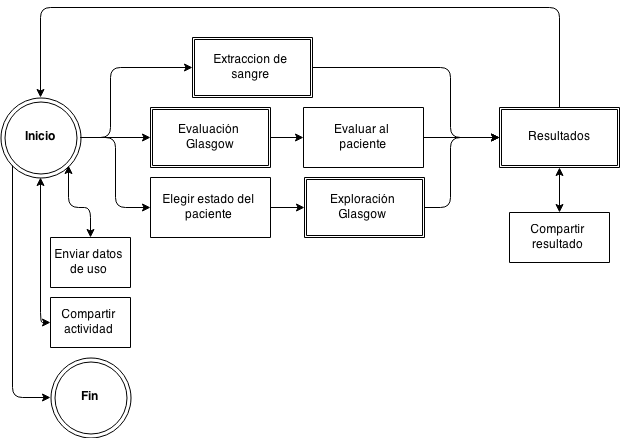
\includegraphics[scale=0.5]{propuesta/grafo_escenas.png}
\caption{Navegación entre escenarios y pantallas. Los escenarios son los
    rectángulos con un borde de dos rayas, y las pantallas tienen un borde con una
    sola raya. Los estados inicial y final se muestran como círculos, notar que
    el estado inicial es además del punto de entrada, un escenario.}
\label{fig:grafo_estados}
\end{figure}

La solución inicia con un escenario denominado \emph{Inicio}, en el cual se
permite al usuario observar los detalles del entorno simulado a la vez que
muestra las opciones que permiten iniciar las diferentes prácticas, compartir
su actividad, enviar los datos de utilización y finalmente salir de la
simulación.

Si el usuario selecciona en el \emph{inicio} la opción \emph{Extracción de
    sangre}, se inicia el escenario denominado \emph{Extracción de sangre}, en
el cual el usuario puede realizar el procedimiento de extracción de sangre, si
el usuario selecciona la opción \emph{Fin}, la simulación termina y se dirige 
al escenario \emph{Pantalla de resultados}.

Al seleccionar la opción \emph{Evaluación Glasgow}, se inicia el escenario
denominado \emph{Glasgow}, donde el usuario debe evaluar a un paciente en el
centro del escenario, si el usuario presiona la opción \emph{Fin} se inicia la
pantalla denominada \emph{Evaluar al paciente}, donde el usuario diagnostica el
estado del paciente, y finalmente al presionar el botón \emph{Fin}, la
simulación finaliza y se inicia el escenario \emph{Pantalla de resultados}.

La opción \emph{Exploración Glasgow} es similar, la diferencia es que antes de
iniciar el escenario \emph{Glasgow}, aparece la pantalla \emph{Elegir estado de
    paciente}, en el cual el usuario selecciona un estado para que el paciente
actué de acuerdo al mismo, luego se inicia la escena \emph{Glasgow} y si el
usuario presiona el botón \emph{Fin}, se inicia el escenario \emph{Pantalla de
    resultados}.

La pantalla de resultados muestra la información acerca de las acciones que
realizó el usuario, proveyendo información a modo de retroalimentación, en esta
pantalla el usuario puede compartir sus resultados por las redes sociales,
reiniciar el escenario y finalmente, puede volver a la \emph{Pantalla de
    inicio}.

A continuación, se describen todos los escenarios, primeramente se da una 
descripción general de los escenarios y se procede a explicar los detalles 
de los mismos, incluyendo las entidades, eventos y acciones que pueden ser realizados 
en el mismo.

\subsection{Inicio}

La solución se inicia con un escenario que esta inspirado en el laboratorio de
enfermería del \Gls{iab}, es la primera experiencia que tiene un
usuario al utilizar la misma, sirve como un menú principal, desde
este punto todas las opciones son accesibles para el usuario, este escenario es
denominado~\emph{Inicio}.

La primera vez que se inicia la solución, se muestra una pequeña ventana
solicitando el número de teléfono del usuario, se utiliza esta información como un
identificador del usuario para así poder asociar la información del mismo con un
alumno en particular.

\subsubsection{Descripción del entorno}
\label{sec:inicio_descripcion}

La escena mostrada como pantalla de inicio de la aplicación muestra como fondo
la sala de un hospital con los elementos típicos de estos lugares, esta es la
que se utiliza como escenografía principal en las escenas de los procedimientos.
Además de este fondo, se muestran varias opciones en forma de botones que serán
descriptas a continuación y un mensaje en donde se recomienda al usuario el uso
de auriculares.

\begin{figure}[H] 
\centering 
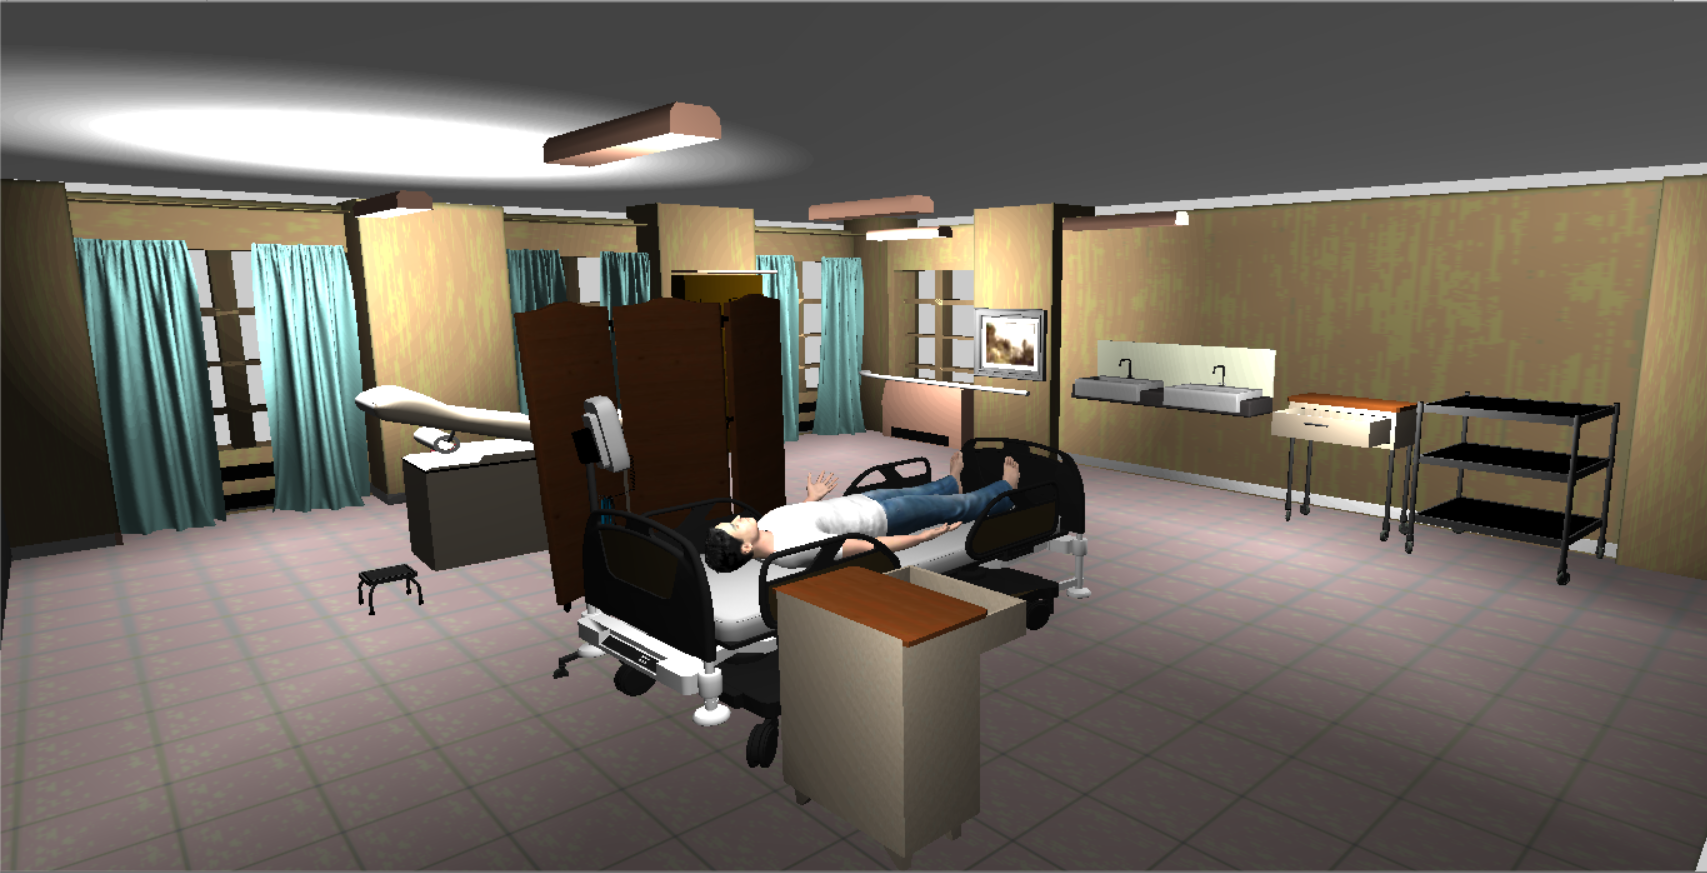
\includegraphics[scale=0.2]{propuesta/sala.jpg}
\caption{Edificio y decoración inspirados en los laboratorios de enfermería del
    \Gls{iab}, este edificio se utiliza para los diferentes escenarios}
\label{fig:sala_perspectiva}
\end{figure}

Se observa en la figura~\ref{fig:sala_perspectiva} la decoración utilizada en
el escenario \emph{Inicio}, mientras se muestran las opciones, se ejecuta una
animación que recorre el escenario mostrando los detalles importantes, como la
camilla, el lector de estadísticas vitales, y demás elementos del escenario.

\subsubsection{Opciones}

Las opciones disponibles en la pantalla de inicio son presentadas en forma de
botones los cuales tienen una breve descripción que identifica la función que
cumplen. 

\begin{itemize}
\item Botón \enquote{Enviar Progreso}: esta función envía toda la información
    acerca de la actividad que el usuario realizó en la aplicación a un servidor
    \emph{backend} que se encarga de almacenar estos datos.
\item Botón \enquote{Salir de la simulación}: esta función permite salir de la
    aplicación.
\item Botón \enquote{Facebook}: esta función permite al usuario ingresar a su
    cuenta de Facebook.
\item Botón \enquote{Extracción de sangre}: esta función permite ingresar a la
    escena correspondiente al procedimiento de extracción de muestras de sangre
    permitiendo al usuario jugar una nueva partida.
\item Botón \enquote{Explorar Glasgow}: esta función permite ingresar a la
    escena correspondiente al procedimiento para explorar las reacción de un
    paciente con un diagnóstico específico de la escala de Glasgow permitiendo
    al usuario jugar una nueva partida, el diagnóstico se selecciona una vez
    presionado este botón a través de la ventana de~\emph{Elegir estado del
        paciente}.
\item Botón \enquote{Evaluar Glasgow}: esta función permite ingresar a la escena
    correspondiente al procedimiento para la valoración y diagnóstico de la
    escala de Glasgow para un paciente con estado aleatorio permitiendo al
    usuario jugar una nueva partida.
\end{itemize}


\subsection{Extracción de muestras de sangre}

A continuación se detallan cada una de las opciones y formas disponibles de
interactuar con la escena del procedimiento de extracción de muestras de sangre.

Los detalles a continuación toman en cuenta las hipótesis definidas
en~\ref{sec:hemocultivo_hipotesis}. 

\subsubsection{Descripción del entorno}

Al seleccionar el procedimiento de extracción de sangre en la pantalla de inicio 
la aplicación inmediatamente muestra la escena del procedimiento, se muestra una 
sala de hospital igual a la de la pantalla de inicio pero con un paciente en una 
de las camas, a este paciente es a quien se le realizará el procedimiento.

La posición inicial de la cámara se ubica en un ángulo en donde se puedan ver 
bien los brazos del paciente para facilitar al usuario la realización del 
procedimiento.


\subsubsection{Entidades}

En la extracción de sangre existen dos entidades principales, el \emph{paciente}
y el \emph{usuario}, cada entidad mantiene un estado independiente de la otra
entidad.

El \emph{paciente} es una entidad con estado complejo, el cual es constantemente
modificado por las acciones del usuario, en resumen, la información que contiene
el paciente es:

\begin{itemize}
    \item \textbf{Jeringas}: un paciente puede tener cero o más jeringas en
        cualquier momento, no se limita la cantidad de jeringas que puede
        insertar el usuario.
    \item \textbf{Manos}: almacena el estado de las manos, el paciente reacciona
        ante peticiones del usuario, puede abrir o cerrar cualquier mano en
        cualquier momento.
    \item \textbf{Torniquetes}: es el conjunto de torniquetes que tiene
        actualmente el paciente, notar que los torniquetes pueden ser colocados
        en cualquier parte del brazo, pero existen lugares \enquote{correctos} y
        lugares \enquote{incorrectos}, la diferencia consiste en la distancia a
        los puntos de extracción, estos lugares están predefinidos.
    \item \textbf{Zonas esterilizadas}: son aquellas áreas del cuerpo que el
        usuario esterilizó, no existe un límite para las zonas esterilizadas.
        Una vez que una jeringa es extraída, una zona esterilizada pasa a estar
        contaminada y a la espera de que el usuario la presione.
    \item \textbf{Zonas presionadas}: son aquellas zonas que, una vez
        contaminadas por la extracción de una jeringa, han sido presionadas por
        el usuario.
    \item \textbf{Contaminado}: define si alguna acción realizada por el usuario
        provocó que el paciente se contamine, existen varias cadenas de eventos
        que pueden hacer que esto ocurra:
        \begin{itemize}
            \item Inyección de una jeringa cuando existe otra inyectada.
            \item Inyección en un lugar inadecuado.
            \item Inyección en un lugar no esterilizado.
            \item Inyección en un brazo cuya mano este abierta.
            \item Inyección fuera del alcance de los torniquetes actuales.
            \item Interacción con el paciente sin que el enfermero tenga la mano
                estéril.
        \end{itemize}
        Es importante notar que este estado no es afectado directamente por una
        acción del usuario, sino por la consecuencia de una acción.
\end{itemize}

El \emph{usuario o enfermero} mantiene un estado en todo momento del cual
dependen sus acciones, por ejemplo, si la mano del enfermero no está
esterilizada, cualquier interacción con el paciente provocará que se
contamine.

\begin{itemize}
    \item \textbf{Manos}: almacena la información acerca de la esterilidad de
        las manos.
    \item \textbf{Guantes, gorro, bata y tapaboca}: almacenan la información
        acerca de los equipamientos que tiene el usuario en un momento dado.
    \item \textbf{Elemento actual}: es el elemento que está activo en
        cualquier momento, un elemento es una herramienta de la vida real,
        como por ejemplo un torniquete, una gaza.
\end{itemize}

\subsubsection{Acciones}

Las acciones que puede realizar el usuario se clasifican en tres, los
\emph{comandos de voz} que simulan una conversación entre el paciente y
enfermero, \emph{las opciones}, que engloban las acciones que puede realizar un
enfermero en cuanto a bioseguridad, y \emph{los elementos} que son las
herramientas que puede utilizar el enfermero durante el procedimiento.

\paragraph{Comando de voz}

Para representar la interacción del usuario con el paciente usando la voz se
implementó un menú que es activado y mostrado en pantalla cuando el usuario
habla, este menú muestra una serie de órdenes que el usuario le diría al
paciente normalmente. Las opciones de menú se detallan a continuación:

\begin{itemize}
    \item \textbf{Explicar procedimiento}: Permite que el usuario explique el
        procedimiento que se va a realizar al paciente. 
\item \textbf{Abrir la mano izquierda}: esta función le indica al paciente que
    abra su mano izquierda, como resultado el paciente realiza esta acción.
\item \textbf{Cerrar la mano izquierda}: esta función le indica al paciente que
    cierre su mano izquierda, como resultado el paciente realiza esta acción.
\item \textbf{Abrir la mano derecha}: esta función le indica al paciente que
    abra su mano derecha, como resultado el paciente realiza esta acción.
\item \textbf{Cerrar la mano derecha}: esta función le indica al paciente que
    cierre su mano derecha, como resultado el paciente realiza esta acción.
\end{itemize}

\begin{figure}[H]
\centering
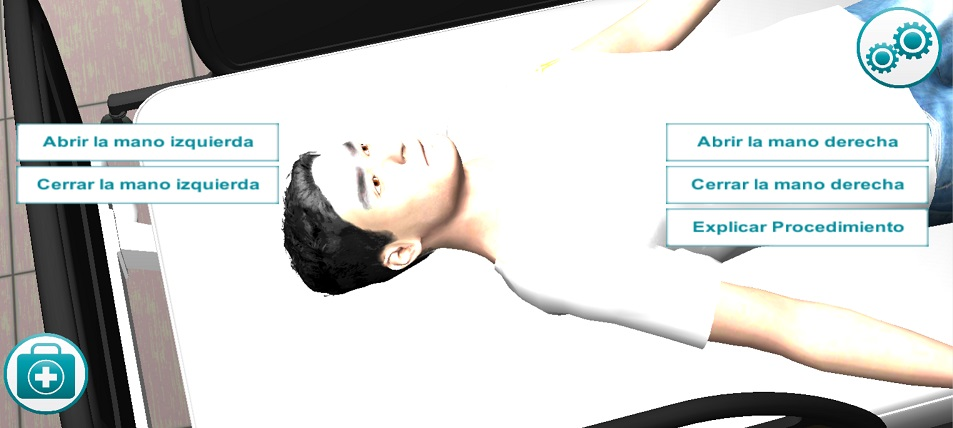
\includegraphics[scale=0.5]{propuesta/hemocultivo_comando_voz.jpg}
\caption{Opciones mostradas al detectar sonido en la escena de extracción
    de sangre.}
\label{fig:hemocultivo_voz_gui}
\end{figure}

En la figura~\ref{fig:hemocultivo_voz_gui} se observan las opciones anteriormente
descritas, este menú aparece inmediatamente después de que el sistema detecte
que el usuario este hablando.

\paragraph{Opciones}

Las \emph{Opciones} son aquellas acciones que puede realizar el usuario y afectan
únicamente al paciente. Representan a los aspectos de bioseguridad, es decir,
acciones como lavarse las manos, calzarse guantes, gorro, bata y tapaboca.

Estas opciones afectan al estado de la entidad \emph{enfermero}.

\paragraph{Elementos}

Los \emph{Elementos} representan las herramientas que utiliza un enfermero
durante el procedimiento, un solo elemento puede ser utilizado en cualquier
momento.


\begin{figure}[H]
\centering
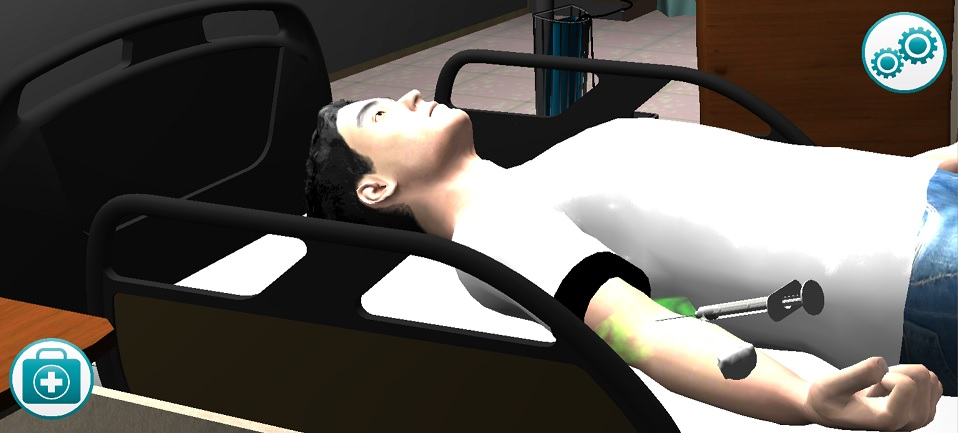
\includegraphics[scale=0.5]{propuesta/hemocultivo_elementos.jpg}
\caption{Interfaz con los elementos en el paciente, se observa el torniquete (es
    un toro negro), la jeringa, una zona esterilizada (el área cerca del
    torniquete) y un algodón para punzar (Cerca de la muñeca, es una figura
    blanca), todo en el brazo derecho.}
\label{fig:hemocultivo_elementos}
\end{figure}

Los elementos, que podemos observar en la
figura~\ref{fig:hemocultivo_elementos}, son:

\begin{itemize}
\item \textbf{Torniquete}: es el primer elemento que se debe usar, para utilizarlo
    , el mismo se activa al presionar una parte del brazo del paciente,
    en ese momento, el torniquete aparece en el brazo del paciente, para
    extraerlo, se debe presionar el torniquete y elegir la opción extraer. En la
    figura~\ref{fig:hemocultivo_elementos} se observa al torniquete como un toro
    negro alrededor del brazo izquierdo.

\item \textbf{Esterilizador}: es un elemento que se utiliza para realizar la
    higienización del punto de punción, para utilizarlo se debe presionar
    cualquier parte del brazo del paciente, a continuación aparece una gaza, la
    cual debe ser agitada con un dedo durante un segundo para que se cree una
    zona estéril, la zona estéril creada, es visible a través de una cápsula
     transparente de color verde.

\item \textbf{Jeringa}: Es el elemento utilizado para realizar la extracción, su
    utilización es similar a la del \emph{Torniquete}, solo que además de la
    opción de extracción tiene dos opciones adicionales.

    A través de un menú contextual, se ofrece la posibilidad de realizar un
    acercamiento, como se observa en la
    figura~\ref{fig:hemocultivo_jeringa_zoom}, en la vista ampliada, se puede
    realizar la extracción de sangre utilizando dos dedos, con el primero se
    presiona el tambor y con el segundo dedo se extrae el émbolo\footnote{El
        tambor es la parte de la jeringa que almacena el fluido, mientras que el
        émbolo es la parte que se utiliza para presionar o succionar el fluido}.
    
\item \textbf{Algodón}: El algodón se utiliza para presionar una zona que
    recientemente fue punzada, para utilizar este elemento, basta con presionar
    el brazo del paciente durante un segundo.

\end{itemize}


\begin{figure}
\centering
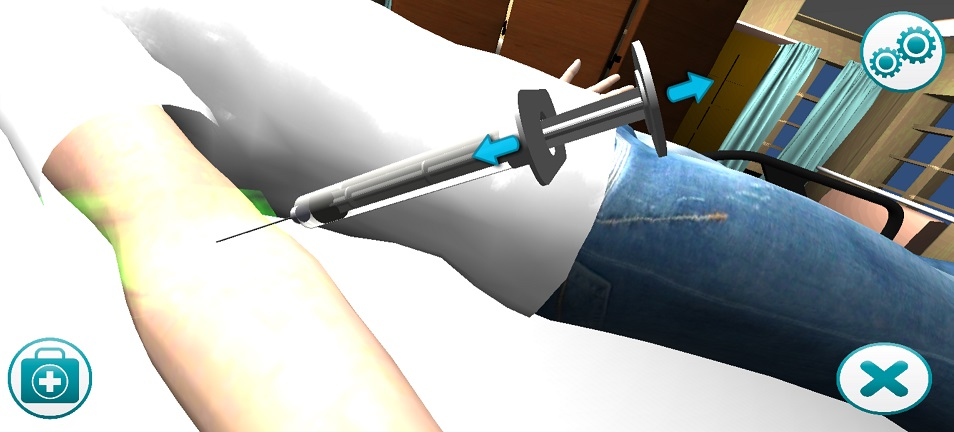
\includegraphics[scale=0.5]{propuesta/hemocultivo_jeringa_ampliada.jpg}
\caption{Vista de la jeringa ampliada, facilitando la extracción de sangre. Se
    agregan flechas azules para facilitar la comprensión del cómo se extrae
    sangre.}
\label{fig:hemocultivo_jeringa_zoom}
\end{figure}



\subsubsection{Reglas para la evaluación durante la ejecución}

%La reglas del procedimiento de extracción de sangre fueron definidas de acuerdo
%a los pasos requeridos según el protocolo del procedimiento y al orden en el que
%son requeridos. Es decir, cada paso del protocolo tiene asociado una regla
%dentro del motor que lo representa y las condiciones asociadas a cada regla
%están determinadas por el orden en que deben realizarse dentro del protocolo.

%Cada regla tiene una o mas condiciones que deben ser cumplidas para que un paso
%del protocolo realizado se considere correcto.

Las reglas definidas dentro de la extracción de sangre definen las acciones
que se deben llevar a cabo para completar el procedimiento, es necesario que
todas las reglas sean cumplidas para obtener un puntaje perfecto.

Cada regla contiene información acerca del estado del progreso del alumno en un
paso en particular, estas reglas pueden tener como dependencias a otras reglas,
es decir, una regla sólo se puede cumplir si una regla anterior se cumple, este
es el caso de las reglas que definen la extracción de un torniquete, la cual
depende de la regla que define la colocación del torniquete.  

Las reglas definen el mecanismo que se utiliza para proveer una retroalimentación
al usuario una vez finalizada la partida, pues la regla almacena información 
acerca del progreso del usuario en cada paso.

A continuación se da una breve descripción de las reglas utilizadas y sus
diversos estados.

\begin{itemize}
\item \textbf{Explicar procedimiento}: define cuando el usuario ha explicado el
    procedimiento, debe ser la primera regla que se cumple, existiendo dos
    estados que no cumplen la condición, cuando no es la primera regla que se
    cumple y cuando el usuario no realizó la acción.

\item \textbf{Higienización de manos}: define sí las manos del enfemero están
    limpias, existen dos estados para esta regla, cuando se lavó las manos y
    cuando no realizó esta acción. Es importante notar que de esta regla
    dependen varias reglas posteriores, es decir, si esta regla no se cumple,
    las reglas de bioseguridad no pueden ser cumplidas.

\item \textbf{Calzar guantes}: este paso es inmediatamente posterior a la
    higienización de las manos, y como este, varias reglas dependen del momento
    en el que se calcen los guantes. Si el paciente se calza los guantes, la
    única forma de equivocarse en este paso es que las manos estén sucias.

\item \textbf{Gorro, bata y tapaboca}: estos tres pasos son similares, pues
    tienen las mismas dependencias y el orden en el que se cumplan no está
    definido, las posibilidades con este paso son:
    \begin{itemize}
    \item Incompleto: si el usuario no se puso el gorro, bata o tapaboca en
        ningún momento de la práctica.
    \item Manos sucias: si la regla \emph{Higienización de manos} no se cumple
        cuando el usuario se vista con el gorro, bata o tapaboca.
    \item Sin guantes: si la regla \emph{Calzar guantes} no se cumple al momento
        de ponerse el gorro, tapaboca o bata. 
    \end{itemize}
    
\item \textbf{Colocar torniquete}: este paso debe ser realizado una vez que el
    usuario tenga el guante calzado, el torniquete puede ser colocado en
    cualquier parte del brazo, pero depende del lugar de punción de la jeringa.
    Así, existen dos casos donde esta regla falla, cuando no se coloca el
    torniquete en ningún lugar, y cuando el torniquete se coloca en un lugar
    inadecuado. Es importante notar que esta regla se activa cuando se realiza
    la punción de la jeringa.

\item \textbf{Cerrar manos}: debe ocurrir después de que se explique el
    procedimiento y antes de que se inserte la jeringa, además deberá ser la
    mano correspondiente al lugar donde se inyectó la jeringa. Así, existen dos
    formas de no realizar correctamente este paso, que la punción haya ocurrido en otro brazo, o
    que la punción no se realizó. Es importante notar que esta regla no se activa
    cuando el usuario solicita al paciente que cierre su mano, sino cuando la
    jeringa es insertada, esto es así pues es importante el estado de la mano
    cuando el usuario realiza la punción.

\item \textbf{Esterilizar zona}: El usuario puede esterilizar varias zonas, pero
    la única zona que activa esta regla, es aquella donde se realizó la punción.
    Así esta regla tiene dos posibles formas de proveer retroalimentación en
    caso de que no se cumpla, que no se esterilizó ningún lugar del cuerpo, o
    que el lugar esterilizado no sea el lugar de punción.

\item \textbf{Realizar punción}: Existen dos casos de error, si el usuario
    inserta la jeringa en un lugar incorrecto (los lugares correctos se definen
    en~\ref{sec:hemocultivo_hipotesis}), y si el usuario no realiza la punción.

\item \textbf{Retirar Torniquete}: esta regla es dependiente de la regla
    \emph{Colocar Torniquete}, y de qué torniquete se retira. Existiendo dos
    casos de error, el usuario retira un torniquete que no activó la regla
    \emph{Colocar Torniquete} (indicando que este es el torniquete correcto), y
    que no se retire ningún torniquete.

\item \textbf{Abrir mano}: una vez realizada la punción, y retirado el torniquete,
    se debe solicitar al paciente que abra sus manos, así, es dependiente de la
    regla \emph{Realizar punción}, y tiene tres casos de error, que la punción
    no se haya realizado, que la mano no se haya cerrado antes, y que la mano
    que se abra no corresponda con la mano que se cerró.

\item \textbf{Extraer Sangre}: depende únicamente de si la jeringa con la cual
    se extrae sangre es la correcta, así hay dos posibles casos de error, que
    la sangre no se haya extraído, y que la regla \emph{Realizar punción} no se
    cumpla.

\item \textbf{Retirar Jeringa}: se controla que la jeringa que se extraiga sea
    la jeringa que cumplió el paso \emph{Realizar punción}, así, existen dos
    casos de error, que la jeringa no hay sido extraída y que se extrajo sangre
    de una jeringa incorrecta.

\item \textbf{Presionar zona de punción}: debe realizarse inmediatamente después
    de \emph{Retirar Jeringa}, y tiene dos casos de error, que la jeringa no
    haya sido extraída, y que la zona presionada no corresponda con la zona de
    punción.

\item \textbf{Quitar bata, gorro y tapaboca}: depende de la regla \emph{Bata,
        gorro y tapaboca}, y de que la jeringa haya sido extraída, si el
    enfermero se extrae la bata, gorro o tapaboca antes de retirar la jeringa, se
    produce un error. Otro caso para que esta regla no se cumpla es que la regla
    \emph{Bata, gorro y tapaboca} no se cumpla.

\item \textbf{Descalzar guantes}: depende de que las reglas \emph{Calzar
        Guantes} y \emph{Retirar jeringa}, así existen dos posibles casos de
    error, que el usuario no se calce los guantes, o que la jeringa no haya sido
    extraída.

\item \textbf{Limpiar manos}: Como paso final, se debe proceder a realizar una
    higienización de manos, este debe ser el paso final, y tiene como
    prerrequisito que todas las reglas anteriores hayan sido lanzadas.

\end{itemize}

\paragraph{Retroalimentación y puntuación final}
\label{sec:puntuacion_hemocultivo}

Cada regla tiene asociado un peso, de acuerdo a la dificultad de realizar el
paso, este peso es utilizado al final de la partida para darle una puntuación al
usuario acerca de su rendimiento en la partida.

Además, un regla puede quedar en uno de diferentes estados al final de la
partida como se mostró anteriormente, cada uno de esos estados posee un
significado en el contexto del procedimiento y por lo tanto tienen información
asociada para que al final de la partida se muestre una retroalimentación
correcta al usuario por paso realizado o no.

\subsubsection{Registro de actividad}

Cada acción que realiza el usuario dentro de la simulación provoca un evento, y
estos eventos son registrados de manera transparente para el usuario.

Existen otros tipos de eventos que no son generados por acciones, por ejemplo,
cuando la simulación termina, el motor de reglas lanza un evento por regla,
indicando su estado.

Un subconjunto de todos los eventos, son registrados en un archivo de texto en
formato \Gls{json}, el mismo es posteriormente enviado a un servidor que
almacena la información de todos los usuarios.

Los eventos registrados, son aquellos que involucran a las opciones, elementos,
utilización de la jeringa, torniquete, higienización, y como un caso especial,
todas las reglas también son registradas (independientemente de si son
satisfactorias o no).

La información que se almacena permite reproducir exactamente todo el desarrollo
de la simulación, con excepción de los movimientos de la cámara. De esta manera,
los datos recabados permiten saber en que tareas los usuarios se encontraron con
un mayor número de inconvenientes.

\subsubsection{Interfaz del usuario}

La interfaz principal de este escenario posee dos menús, uno a cada lado de la
pantalla, las opciones son representadas como botones que poseen una imagen
intuitiva que representa la función que realizan. 

\begin{figure}
\centering
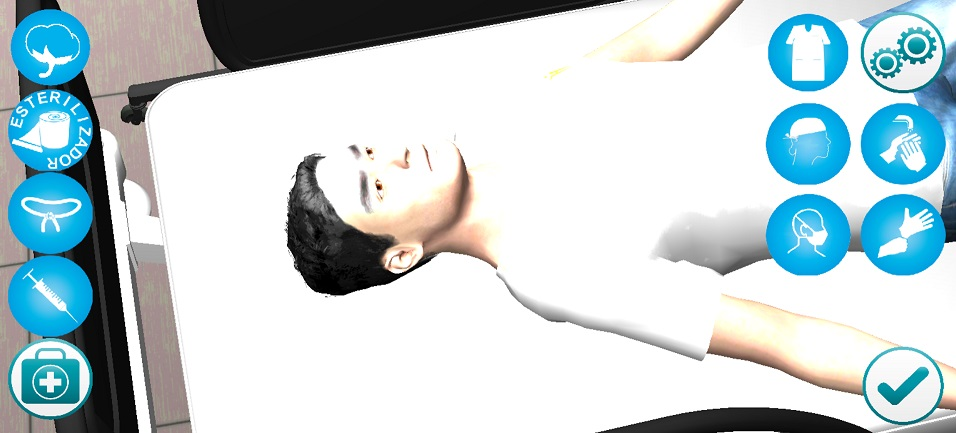
\includegraphics[scale=0.5]{propuesta/hemocultivo_gui.jpg}
\caption{Vista de la interfaz principal del escenario \emph{Extracción de
        sangre}, con todas las opciones desplegadas.}
\label{fig:hemocultivo_gui}
\end{figure}


En la figura~\ref{fig:hemocultivo_gui} se observa la interfaz, se muestra en el
centro al paciente, y las diferentes opciones que tiene el usuario para
interactuar con el paciente y consigo mismo como enfermero.

Existen dos opciones principales dentro de la interfaz, en la parte superior
derecha se encuentra el menú \emph{Opciones} y en la parte superior izquierda, el menú
\emph{Elementos}.

Al presionar el menú \emph{Opciones} aparecen las distintas
acciones que puede realizar el usuario en cuanto a aspectos de bioseguridad, el 
lavado de manos es idempotente, es decir no importa cuantas veces se presione, el 
resultado será el mismo, en cambio los demás botones (bata, guante, tapaboca y gorro)
representan la acción de calzar/descalzar, es decir, la primera vez que se presiona
la opción bata, el estado del enfermero cambia a \emph{Con Bata}, si se presiona una
segunda vez, el estado cambia a \emph{Sin Bata}.

En el menú \emph{Elementos} se despliegan opciones que representan a lo elementos que se
utilizan para realizar el procedimiento, una vez presionado un elemento queda
seleccionado (simulando que es la herramienta que el enfermero tiene en la mano
en ese momento), sólo un elemento puede ser seleccionado a la vez. Si el mismo
botón se vuelve a presionar inmediatamente después de haber sido presionado, el
elemento se des-selecciona (simulando que el enfermero dejó la herramienta).

Adicionalmente, existen dos indicadores del estado del paciente, en la parte
inferior derecha, denominados \emph{Indicadores de bioseguridad}, se muestran
iconos representando los elementos que tiene actualmente el enfermero, estos
incluyen los gorros, bata y tapaboca. El elemento que actualmente esta
seleccionado se muestra en la parte superior izquierda de la pantalla, a
diferencia de los indicadores de bioseguridad, se muestra un único icono a la vez.

Para la utilización de los elementos, existe un menú contextual\footnote{Un menú
    que se despliega al presionar un elemento, es contextual pues varía de
    acuerdo al elemento seleccionado.}, que lista las opciones disponibles por
elemento, como se observa en la figura~\ref{fig:hemocultivo_torniquete_cm}.

\begin{figure}
\centering
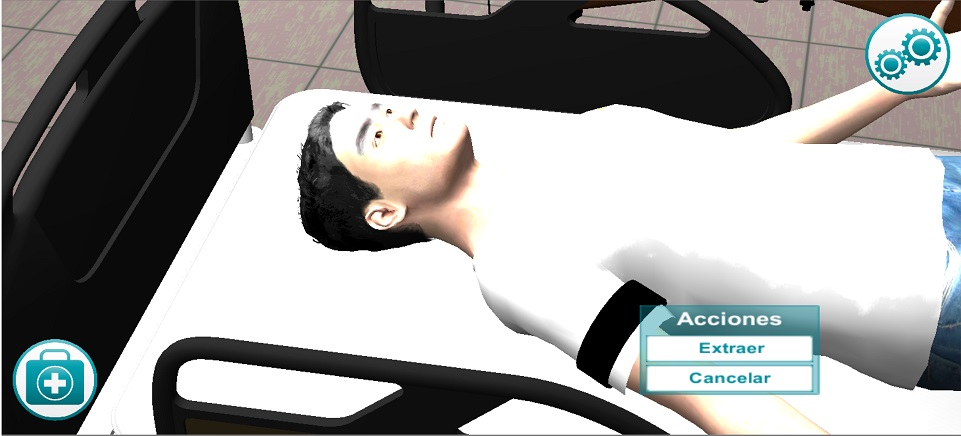
\includegraphics[scale=0.5]{propuesta/hemocultivo_contextual.jpg}
\caption{Menú contextual del elemento torniquete.}
\label{fig:hemocultivo_torniquete_cm}
\end{figure}

\subsection{Valoración de la escala de Glasgow}


La escena  \emph{Valoración de la escala de Glasgow} busca simular el
comportamiento de un paciente con daño cerebral, por ello se presenta en dos
modos distintos, en la primera, el usuario no conoce el estado del paciente,
este modo se conoce como \emph{Evaluar Glasgow}, y en su segundo modo, el
usuario elige el estado del paciente antes de iniciar la escena, esto modo
se conoce como \emph{Exploración Glasgow}. 

La reducida cantidad de diferencias entre ambos modos de la práctica permiten
que ambas sean descritas en esta sección, las características explicadas son
comunes para ambas, salvo que se especifique lo contrario.

En el modo \emph{Exploración Glasgow}, antes de iniciar la práctica, se le
permite al usuario seleccionar el estado del paciente mediante una interfaz, en
cambio, en el modo \emph{Evaluar Glasgow}, el estado del paciente no se conoce
de antemano y será responsabilidad del usuario determinarlo.

La escena se inicia mostrando un paciente acostado en una camilla, de manera
similar a la escena \emph{Extracción de sangre}, la principal diferencia es que
el paciente no se encuentra en ninguna posición en particular, simplemente esta
acostado en la camilla.

Existe una pantalla particular dentro de esta escena, conocida como
\emph{Pantalla de Diagnóstico}, esta pantalla, permite al usuario ingresar su
diagnóstico del paciente, contiene cuatro preguntas básicas, la valoración
motora, verbal, ocular y general de acuerdo a lo definido en~\ref{sec:glasgow} y
a las hipótesis definidas en~\ref{sec:glasgow_hipotesis}.

\emph{Exploración Glasgow}.

\subsubsection{Entidades}

Al igual que en \emph{Extracción de sangre}, existen dos entidades principales,
pero en esta escena, el enfermero no almacena información alguna, y el
paciente sólo almacena su estado, que se define al inicio. De esta forma, las
entidades no se modifican en ningún momento.

La información almacenada por la entidad paciente es su estado motor, verbal y
ocular, el cual es un conjunto de números, cuyos posibles valores se definen en
en~\ref{sec:glasgow_protocolo}, la definición de estos números varían de acuerdo
al tipo de la escena:

\begin{itemize}
    \item \textbf{Exploración}: la escena de exploración se inicia con la
        \emph{Pantalla de diagnóstico}, donde el usuario selecciona el estado
        del paciente que desea, este estado se mantendrá constante durante toda
        la escena.
    \item \textbf{Evaluación}: al inicio se crean tres números de manera
        aleatoria, el algoritmo que crea estos valores, lo hace de tal manera
        que el estado del paciente es consistente, por ejemplo, el paciente
        nunca tendrá un estado verbal \enquote{Orientado} (valor 5 en la escala)
        y un estado ocular \enquote{Ausente} (valor 1 en la escala), pues esto
        no tendría sentido, si no puede abrir los ojos (estado
        \enquote{ausente}), no puede saber donde esta (estado
        \enquote{orientado}).
\end{itemize}

Aunque el estado de las entidades no se modifique, esto no significa que no
puedan realizar acciones entre ellas, sino que estas acciones y los eventos
generados no alteran el estado de las entidades.

\subsubsection{Acciones} 

Las acciones se clasifican en dos tipos, los \enquote{comandos de voz} y las
\enquote{opciones a través de menú contextual}. 

\paragraph{Menú Contextual}

Las opciones a través del menú contextual se relacionan a acciones que puede
realizar el enfermero sobre una parte particular del cuerpo del paciente, en las
extremidades, el menú despliega una sola opción, la cual es \emph{Pinchar}, que
provoca que el enfermero realice un estímulo doloroso al paciente, el
paciente reacciona ante este estímulo dependiendo de su valoración motora y
ocular. 

\begin{itemize}
    \item Si el estado ocular del paciente es \enquote{Al dolor}, el paciente
        abrirá los ojos inmediatamente después de que se presione la opción. 
    \item  La respuesta motora varía de acuerdo a su estado, si el mismo es
        \enquote{Localiza}, el paciente mueve sus manos hasta el origen del
        dolor, si el estado es \enquote{Retira}, moverá la extremidad que
        sufrió el estímulo lejos de su posición inicial, si es
        \enquote{Flexión anormal}, el paciente reaccionará comprimiendo el
        cuerpo, indistintamente de la ubicación del estímulo doloroso, y si el
        estado es \enquote{Extiende}, el paciente extenderá el cuerpo.
\end{itemize}

\paragraph{Comandos de voz}

Las opciones disponibles a través de los comandos de voz, simulan una
interacción verbal entre el enfermero y el paciente, y se agrupan en tres
tipos, verbales, oculares y motoras.

Las preguntas y posibles respuestas de tipo \emph{verbal}, se pueden ver en la
tabla~\ref{tab:glasgow_opciones_respuesta}. 

\begin{table}[H]
\centering
\begin{tabulary}{1.2\textwidth}{LCCCCC}
\toprule
\textbf{Pregunta} & \textbf{Orientado} & \textbf{Confusa} & \textbf{Palabras
    inapropiadas} & \textbf{Palabras incomprensibles} & \textbf{Ausente} \\
\midrule
¿Qué día es? & El día de la semana actual & Cualquier día de la semana menos el
correcto & La respuesta a otra pregunta en estado orientado & Gritos, gruñidos y
quejidos & No emite sonido \\
¿Cuál es su nombre? & \emph{Carlos Benitez} & Respuesta coherente sin mencionar
su nombre & Respuesta a otra pregunta en estado orientado & Gritos, gruñidos y
quejidos & No emite sonido \\
¿Donde se encuentra? & \emph{En una cama de hospital} & \emph{En mi dormitorio} &
Respuesta a otra pregunta en estado orientado & Gritos, gruñidos y quejidos & No
emite sonido \\
\bottomrule
\end{tabulary}
\caption{Posibles respuestas de acuerdo al estado verbal del paciente.}
\label{tab:glasgow_opciones_respuesta}
\end{table}

Las opciones del menú por comandos de voz del tipo \emph{motor}, son cuatro: 

\begin{itemize*}
    \item Mueva el brazo
    \item Mueva la pierna
    \item Mueva la mano
    \item Mueva la cabeza
\end{itemize*}

A diferencia de las opciones verbales, estas no tienen una respuesta sonora, en
cambio, si el estado motor es \enquote{Obedece},el paciente reacciona moviendo
una extremidad, en caso contrario, el paciente no realiza acción alguna.

Finalmente, existe una opción \emph{ocular}, la cual es \enquote{Abra sus ojos por
favor}, la cual no tiene una respuesta sonora, y sólo si el paciente tiene un
estado ocular \enquote{Al hablar} abre los ojos, en caso contrario, no realiza
acción alguna.

\subsubsection{Pantalla de diagnóstico}

Una vez que el usuario decida que está listo para dar un diagnóstico, procede a
finalizar la escena, en ese momento se presenta una pantalla donde el mismo
puede diagnosticar al paciente, como se observa en la
figura~\ref{fig:glasgow_gui_resultados}.

Las opciones presentadas al usuario son cuatro, puntuación verbal, ocular,
motora y un diagnóstico del estado de conciencia del paciente. Estos valores
se describen en~\ref{sec:glasgow_protocolo}.

\begin{figure}[H]
\centering
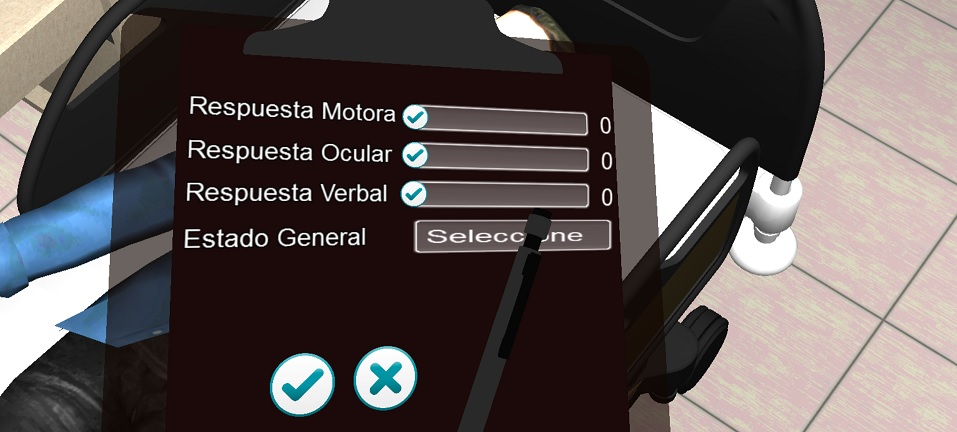
\includegraphics[scale=0.5]{propuesta/glasgow_diagnostico.jpg}
\caption{Vista de la \emph{Pantalla de diagnóstico}, donde el usuario puede
    asignar una puntuación a cada aspecto analizado del paciente.}
\label{fig:glasgow_gui_resultados}
\end{figure}

En el modo \emph{Evaluación Glasgow}, esta misma pantalla se utiliza la inicio
de la escena para que el usuario pueda seleccionar el estado deseado del
paciente.

La única diferencia que existe entre la \emph{Pantalla de diagnóstico} entre la
exploración y la evaluación, es que en la evaluación, los posibles valores para
cada aspecto a diagnosticar van de $0$ a $8$, y en la exploración, son los
valores mínimos y máximos válidos\footnote{Los valores máximos se definen
    en~\ref{sec:glasgow_protocolo} y son $4$ (ocular), $5$ (verbal) y $6$
    (motora)}.

\subsubsection{Valoración}
\label{sec:puntuacion_glasgow}

Para la evaluación del rendimiento del usuario al momento de llevar a cabo el
procedimiento de valoración de la escala de Glasgow se tuvo un enfoque
completamente diferente al del procedimiento de extracción de sangre debido a la
naturaleza propia del procedimiento. 

Como se explicó anteriormente, el paciente puede estar en ciertos estados
específicos dentro de la escala, y además dentro de cada estado reacciona de una
forma en particular, por lo tanto, al inicio de la partida un componente interno
de la aplicación selecciona de forma aleatoria un estado para el paciente, de
forma tal que cada vez que una partida sea jugada no se repitan los estados de
forma seguida.

El estado aleatorio del paciente es guardado en una variable que no es
modificada hasta que se reinicie la partida. Al final de la partida, la
aplicación pide al usuario que valore el estado del paciente que le fue
presentado, una vez que el usuario confirme su respuesta la aplicación la
compara con el estado guardado y de esta forma puede informar al usuario acerca
de su rendimiento en el diagnóstico.

Además, cada posible respuesta dada por el usuario contiene información
relacionada al contexto del procedimiento y a la situación actual presentada, la
cual, es utilizada como retroalimentación al final de la partida. La puntuación
final depende de la cantidad de valoraciones correctas dadas por el usuario
para la respuesta verbal, motora, ocular y nivel de gravedad del paciente.

\subsubsection{Registro de actividad}

Al igual que en la escena de \emph{Extracción de sangre}, las acciones del usuario
son registradas en un archivo con formato \Gls{json} y enviadas a un servidor
que almacena la información acerca de todos los usuarios.

Se almacena además, el diagnóstico del usuario, la puntuación del mismo y el
estado inicial del paciente, así como el modo de la escena (evaluación o
exploración).

\subsubsection{Interfaz de usuario}

La interfaz de usuario, como se observa en la figura~\ref{fig:glasgow_gui}, es
muy sencilla, se compone de solo una opción permanente, la cual permite al
usuario finalizar la escena y mostrar la \emph{Pantalla de diagnóstico}. Se
observan además, las opciones que se despliegan cuando la solución detecta que el
usuario emite palabras, conocidas como \emph{Comandos de Voz}, que permiten al
mismo interactuar con el paciente.

\begin{figure}[H]
\centering
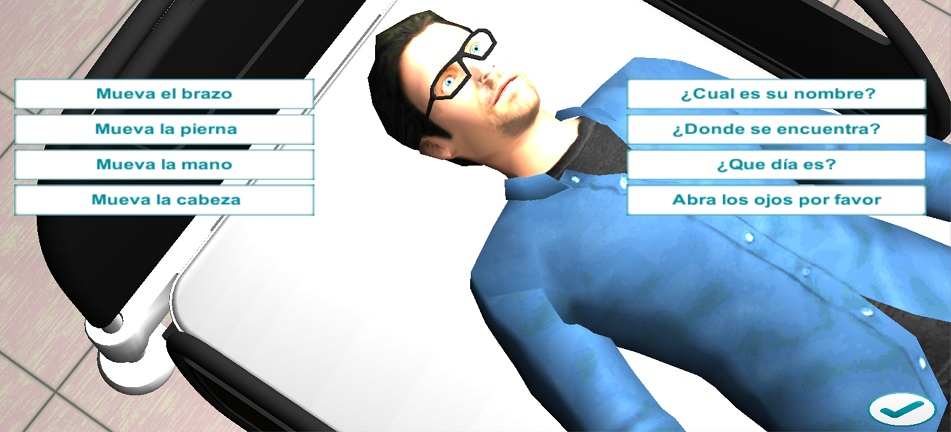
\includegraphics[scale=0.5]{propuesta/glasgow_comandos_voz.jpg}
\caption{Interfaz de la escena \emph{Evaluación de Glasgow}, se observan los
    \emph{comandos de voz}, así como la opción que permite finalizar la escena
    (esquina inferior derecha).}
\label{fig:glasgow_gui}
\end{figure}

Además se ve en la interfaz, al paciente, que es el foco principal de la cámara.

\subsection{Pantalla de resultados}

Al finalizar ambas escenas, se presenta una pantalla de resultados, la cual es
la encargada de mostrar toda la información que fue recabada durante la escena,
esta información incluye los pasos correctos e incorrectos que realizó el
usuario.

\begin{figure}[H]
\centering
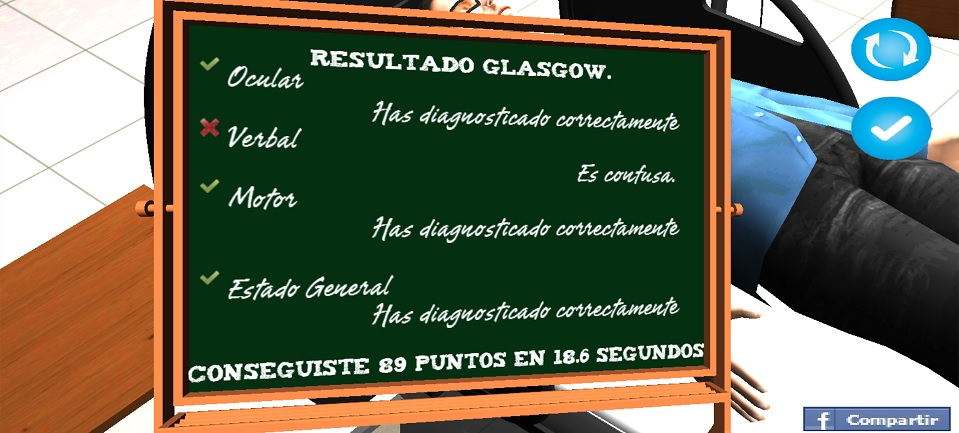
\includegraphics[scale=0.5]{propuesta/resultado_glasgow.jpg}
\caption{Pantalla de resultados mostrando los pasos correctos e incorrectos, en
    la escena \emph{Glasgow}.}
\label{fig:resultados_glasgow}
\end{figure}

Se observa en la figura~\ref{fig:resultados_glasgow} el diseño de la
pantalla, el título es la escena actual, en el pie se observa un resumen de la
puntuación, y el tiempo que duró la escena.

Se lista de manera ordenada los pasos en la parte izquierda de la pantalla, y en
la parte derecha se muestra información relevante acerca del motivo por el cual
no se cumplió cada paso o es caso contrario, se indica que el pao fue realizado 
correctamente.

Adicionalmente a la información de la sesión, se permite al usuario reiniciar la
escena, ir al menú, y compartir sus logros en las redes sociales.

\subsubsection{Retroalimentación}

La retroalimentación se logra a través de la pantalla de resultados, en ella se
presenta información detalla de lo que realizó el usuario. 

Si el usuario realizó de manera incorrecta un paso del procedimiento, esta
información está contenida en una regla (\emph{Extracción de Sangre}), o en el
estado inicial del paciente (\emph{Evaluación de Glasgow}).

\begin{figure}[H]
\centering
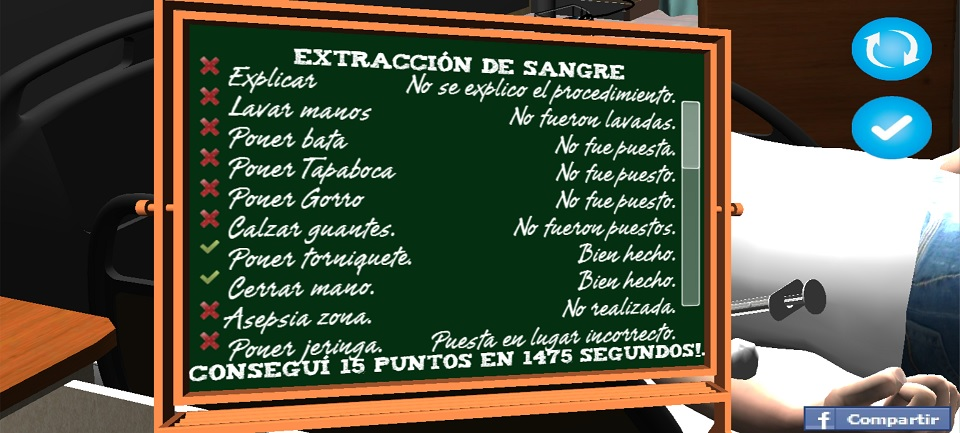
\includegraphics[scale=0.5]{propuesta/resultado_hemocultivo.jpg}
\caption{Pantalla de resultados mostrando los pasos correctos e incorrectos en
    la escena \emph{Extracción de sangre}.}
\label{fig:resultados_hemocultivo}
\end{figure}

Como se observa en la figura~\ref{fig:resultados_hemocultivo}, el paso
\enquote{Poner Jeringa}, contiene la siguiente información \enquote{Puesta en un
    lugar incorrecto}, esto le indica al usuario, que el lugar donde la jeringa
fue insertada era incorrecto, otro posible valor de retroalimentación es
\emph{Jeringa no insertada}.

\subsubsection{Gamificación}

En esta pantalla además se observan opciones que son estudiadas por la
\emph{Gamificación}, entre ellas observamos la puntuación total, el tiempo
utilizado y la utilización de redes sociales.

Si el usuario presiona el botón \enquote{Facebook}, se despliega el menú de
dicha red social, permitiendo que el mismo pueda agregar un mensaje
personalizado y el resultado de la sesión se comparta con el texto \enquote{Conseguí 15 puntos
    en 1475 segundos, en la \emph{Escena Extracción de sangre} jugando con
    YAVE}.


%! TEX root = ../main.tex
\section{Evaluación en tiempo de ejecución}

Las acciones realizadas por los usuarios dentro de la aplicación son evaluadas para determinar si realizo o no el procedimiento de manera correcta y así brindarle información al usuario sobre su rendimiento.

En esta sección se explica como son evaluados las acciones de los usuarios para los diferentes procedimientos simulados.

\subsection{Extracción de muestras de sangre}

Para la evaluación de las acciones del usuario en este procedimiento se utilizo un motor de reglas denominado "Acciones condicionadas por eventos". A continuación se explica en detalle cada aspecto relacionado tanto al motor como a la forma de evaluación del rendimiento del usuario.

\subsubsection{Acciones condicionadas por eventos}

Un evento es la ocurrencia de un hecho en particular, y son identificados por un
nombre y un conjunto de parámetros, por ejemplo, cuando un evento es cuando el
enfermero inserta una Jeringa, el nombre de este evento es
\emph{''jeringa.inserted''}, y sus parámetros podrían ser el lugar y el tiempo
de la inserción, así, la influencia del estudiante en la simulación es una
sucesión de eventos.

Por cada acción que realiza el usuario dentro de la simulación, existe un evento
relacionado, por consiguiente, es razonable estudiar algunos eventos para
determinar si los pasos realizados corresponden con los deseados. 

Para determinar si una sucesión de eventos es la correcta, se definen reglas,
una regla es una asociación de una condición y una acción, la condición define
si el entorno es el adecuado para realizar una acción, la cual es un
procedimiento que realiza la lógica deseada.

Las \gls{eca} son aquellas que son activadas una vez que se cumplen determinados
eventos\cite{bailey2004event}. En las bases de datos relacionales, son conocidos
como triggers, es decir, una base de datos relacional (u orientada a objetos) es
un motor de reglas \gls{eca}\cite{bailey2004event}\cite{behrends2006combining}.

Las mismas pueden ser utilizadas para notificar que un determinado conjunto de
eventos ha ocurrido\cite{bailey2004event}, así como servir para almacenar
información acerca de la utilización de un determinado recurso.


\paragraph{Motivación}

Las reglas del tipo \gls{eca} permiten reaccionar a determinados eventos, en
forma de una única regla, la cual facilita la declaración de las
mismas\cite{bailey2004event}.

Son principalmente útiles para analizar el comportamiento en tiempo real de un
sistema en una forma
reactiva\cite{bailey2004event}\cite{de2001eca}\cite{bailey2002analysis}, esta
característica esta impulsada principalmente por que son ejecutadas después de
la ocurrencia de un evento, y el entorno no es modificado, pudiendo así acceder
al mismo entorno que el qué lanzo el evento.

Definir si las acciones de un usuario son correctas utilizando un motor
\gls{eca} es sencillo desde el punto de vista que sólo se deben definir un
conjunto de acciones que se deben realizar, y agregar una acción que verifica si
los pasos realizados fueron los correctos.

\paragraph{Declaración}

Una \gls{eca}, se define como\cite{bailey2004event}\cite{behrends2006combining}:

\begin{center}
	 Cuando ocurren una serie de \emph{eventos}, y se cumple una
	 \emph{condición}, entonces realizar una \emph{Acción}.
\end{center}

Los \emph{eventos} determinan cuando una regla debe ser activada, los mismos se
dividen en dos categorías\cite{behrends2006combining}, primitivos y compuestos,
los primeros son detectables, por ejemplo, cuando se inserta una jeringa, y los
compuestos, son la combinación de uno o más
primitivos\cite{bailey2004event}\cite{behrends2006combining}. Los eventos
compuestos, se unen mediante:
\begin{enumerate*}[label=\itshape\alph*\upshape)]
\item conjunción (\emph{y}),
\item disyunción (\emph{o}), y
\item secuencia (\emph{entonces}).
\end{enumerate*}
Sin embargo, no siempre son necesarios todas las posibles combinaciones, y las
combinaciones sencillas son más fáciles de optimizar y
probar\cite{bailey2004event}.

La \emph{condición} de una regla determina si el entorno es el necesario para que la
regla sea activada, en esta condición el entorno que lanzó el evento esta
disponible.

La \emph{acción} a ejecutar describe la lógica que debe ser ejecutada cuando se han
lanzado los eventos y la condición de la regla se ha cumplido.

\paragraph{Dependencia entre reglas}

Las reglas pueden depender de otras reglas, lo cual se puede ver como que la
finalización de una regla es un evento que otra regla espera para poder ser
activada.

Las reglas pueden agregar información a un contexto compartido por todas las
reglas, de esta manera, se puede pasar parámetros entre distintas reglas, por
ejemplo, la regla \emph{Retirar Torniquete}, depende de la regla \emph{Insertar
Torniquete}, pero debe responder solamente al torniquete que ha activado
la regla de inserción, es decir, el usuario puede extraer varios torniquetes, y
la regla no debe activarse, hasta que se extraiga el torniquete que activo la
primer regla.

Así, la regla \emph{Retirar Torniquete} depende de la regla \emph{Insertar
Torniquete}, y esta relación entre reglas, se da en dos
formas\cite{bailey2004event}:

\begin{itemize}
\item  \emph{Dependencia fuerte:} la regla \emph{Retirar Torniquete} solamente podrá
	ser elegida para ser lanzada cuando la regla \emph{Insertar Torniquete}
	haya sido cumplida.
\item  \emph{Dependencia de contexto}: la regla \emph{Retirar Torniquete} no se
	activará cuando los eventos a los que escucha se terminen, sino cuando
	los eventos a los que escucha sean lanzados con los parámetros adecuados
	(se extraiga el torniquete que lanzo la regla de inserción).
\end{itemize}

\paragraph{Representación}

La definición de las reglas se realiza de la siguiente forma;
\begin{algorithm}[H]
\caption{Creación de regla de verificación de calzado de guantes}
\label{alg:rule:guante}
\lstset{style=sharpc}
\begin{lstlisting}
Rule.New("Regla de verificacion de calzado de guantes").
     When("enfermero.guantes.calzar").
     Then(e => e.Patient.ManosLimpias()).
\end{lstlisting}
\end{algorithm}
%TODO agregar indice de algoritmos

La regla anterior controla que el estudiante ha realizado la acción ``Calzarse
los guantes'', y en ese momento tenga las manos limpias, la variable \emph{e},
es el entorno, y a través de la propiedad \emph{Patient} obtiene el estado del
paciente en ese momento.

\paragraph{Modelo de ejecución}

Para ejecutar un motor de reglas del tipo \gls{eca}, se debe tener en cuenta
principalmente dos factores, 
\begin{enumerate*}[label=\itshape\alph*\upshape)]
\item  Como se verifica el cumplimiento de cada regla, y, 
\item  Que ocurre cuando varias reglas son lanzadas al mismo tiempo
\end{enumerate*}.

Para ambos casos se puede tomar un enfoque \emph{inmediato}, es decir que
inmediatamente cuando se lanza un evento, o se cumple una condición, se ejecuta
la regla. Además existen otros dos modos de ejecución, \emph{deferida}, y
\emph{desacoplada}, en la primera, se espera hasta que el lanzador del evento
culmine su trabajo, y luego se ejecuta la regla, pero en la misma unidad de
trabajo, mientras que en la ejecución desacoplada, se encolan los trabajos y
otro hilo es el encargado de ejecutar las reglas. Estos modos están inspirados
en las bases de datos relacionales, el deferido se ejecuta en la misma
transacción, y el desacoplado, inmediatamente después de que la transacción
termine\cite{bailey2004event}.

La propuesta implementada, utiliza una ejecución inmediata, principalmente por
la sencillez de las reglas, es decir, las reglas no realizar un proceso complejo,
solamente controlan el estado del entorno y lo validan.

Además, la ejecución inmediata es importante por que el entorno no sufre
modificaciones entre el evento lanzado y la ejecución de la regla, según
\cite{bailey2004event}, este es el factor más importante para determinar el tipo
de ejecución deseado.



\paragraph{Estados de una regla}

Una regla puede estar en uno de los siguientes estados:

\begin{description}
\item[BEGIN] Es una regla que recién fue creada, no realiza ninguna
	acción.
\item[WAITING\_FOR\_RULE] Es un estado en el que esta esperando que otras reglas
	sean lanzadas. En este estado, es un suscriptor de las reglas por la que
	espera, y no forma parte del ciclo de ejecución del motor de reglas.
\item[WAITING\_FOR\_EVENT] Es un estado en el que esta escuchando a que sean
	lanzados los eventos a los que escucha, este es el estado principal. En
	este estado, es un suscriptor de los eventos por los que espera, y no
	forma parte del ciclo de ejecución del motor de reglas. Se diferencia
	del estado anterior, en que los eventos escuchados pueden ser lanzados
	por cualquier objeto del entorno, no necesariamente una regla.
\item[WAITING\_FOR\_CONDITION] La regla ya no espera por ningún evento y las
	reglas de las que depende ya han sido lanzadas, se verifica cada cierto
	tiempo si el entorno cumple con una condición definida. 
\item[FINISH] La regla ha sido lanzada, con un resultado no determinado, se pudo
	haber cumplido, como no, es el estado final de una regla. Cuando una
	regla llega a este estado, se lanza su evento de finalización.
\end{description}

Una regla puede estar en solo un estado, y solamente se permite que el estado
avance, desde \emph{BEGIN} hasta \emph{FINISH}.


\paragraph{Ciclo de vida}

Cuando una regla es definida, y insertada al motor de reglas, inmediatamente
pasa al estado \emph{BEGIN}, luego se verifica si la misma depende de otras
reglas, sí este es el caso, pasa al estado \emph{WAITING\_FOR\_RULE} y escucha a
los eventos de finalización de las reglas anteriores.

Una vez que las reglas anteriores han sido finalizadas, la regla pasa al estado
\emph{WAITING\_FOR\_EVENT} sí deben escuchar por algún evento, en caso contrario
pasan al estado \emph{WAITING\_FOR\_CONDITION}.

Una vez que la regla está en estado \emph{WAITING\_FOR\_CONDITION}, pasa a un
motor que ejecuta su condición cada cierto tiempo, si la condición se cumple, la
regla se ejecuta, y la misma pasa a estado \emph{FINISH}, momento en el cual
notifica a las reglas que dependen de ella que ha sido lanzada.

Una vez que la regla esta en estado \emph{FINISH}, la misma sale del esquema de
ejecución, y solo esta disponible para obtener resultados.

Según el ejemplo de la regla definida en el código\ref{alg:rule:guante}, la
regla al terminar de ser construida pasa a estado \emph{BEGIN}, al no depender
de otras reglas, pasa inmediatamente al estado \emph{WAITING\_FOR\_EVENT},
cuando es lanzado el evento, la regla ejecuta la acción y pasa al estado
\emph{FINISH}.

\paragraph{Motor de ejecución}

Un motor de reglas \gls{eca}, requiere de un proceso que evalúe constantemente
las reglas para verificar si las mismas deben ser lanzadas o
no\cite{bailey2004event}\cite{galton2002two}, este motor puede utilizar el
algoritmo de RETE\cite{de2001eca} para realizar esta verificación, en la
propuesta presentada, la cantidad de reglas definidas, y la no dependencia
circular entre ellas, hace innecesario la implementación de tal
algoritmo\cite{de2001eca}. 

El motor de reglas actúa sobre aquellas reglas en estado
\emph{WAITING\_FOR\_CONDITION} e invoca al procedimiento que se encarga de
validar si la regla puede ser activada (el procedimiento es único por cada
regla), si el mismo determina que la regla puede ser lanzada, el motor ejecuta
la acción de la regla y modifica el estado de la regla a \emph{FINISH}.


\subsubsection{Definición de reglas}

La reglas del procedimiento de extracción de sangre fueron definidas de acuerdo a los pasos requeridos según el protocolo del procedimiento y al orden en el que son requeridos. Es decir, cada paso del protocolo tiene asociado una regla dentro del motor que lo representa y las condiciones asociadas a cada regla están determinadas por el orden en que deben realizarse dentro del protocolo.

Cada regla tiene una o mas condiciones que deben ser cumplidas para que un paso del protocolo realizado se considere correcto.

\subsubsection{Retroalimentación y puntuación final}

Cada regla tiene asociado un peso, de acuerdo a la dificultad de realizar el paso, este peso es utilizado al final de la partida para darle una puntuación al usuario acerca de su 
rendimiento en la partida.

Además, un regla puede quedar en uno de diferentes estados al final de la partida como se mostró anteriormente, cada uno de esos estados posee un significado en el contexto del procedimiento y por lo tanto tiene información asociada para que al final de la partida se muestre una retroalimentación correcta al usuario por paso.

\subsection{Valoración de la escala de Glasgow}

Para la evaluación del rendimiento del usuario en el momento de llevar a cabo el procedimiento de valoración de la escala de Glasgow se tuvo un enfoque completamente diferente al del procedimiento de extracción de muestras
de sangre debido a la naturaleza propia del procedimiento. 

Como se explico anteriormente, el paciente puede estar en ciertos estados específicos dentro de la escala, y además dentro de cada estado reacciona de un forma en particular por lo tanto, al inicio de la partida
un componente interno de la aplicación selecciona de forma aleatoria un estado para el paciente, de forma tal que cada vez que una partida sea jugada no se repitan los estados de forma seguida.

El estado aleatorio del paciente es guardado en una variable que no es modificada hasta que se reinicie la partida. Al final de la partida, la aplicación pide al usuario que valore el estado del paciente que le fue presentado, una vez que el usuario confirme su respuesta la aplicación la compara con el estado guardado y de esta forma puede informar al usuario acerca de su rendimiento en el diagnostico.

Además, cada posible respuesta dada por el usuario contiene información relacionada al contexto del procedimiento y a la situación actual presentada la cual es utilizada como retroalimentación al final de la partida. La puntuación final dada depende de la cantidad de valoraciones correctas dadas por el usuario para la respuesta verbal, motora, ocular y nivel de gravedad del paciente.










\section{Inconvenientes de diseño}

Los mayores inconvenientes de diseño de la aplicación se dieron en el momento de
validar tanto el contenido de la aplicación como la interfaz de usuario, para
sobrellevar estos inconvenientes fueron requeridos la intervención de terceros.

A continuación se explica en detalle cada uno de los casos.

\subsection{Interfaz de usuario}

Como parte del diseño y desarrollo de la solución se realizó una prueba de
interfaz de usuario con alumnos de la carrera de Ingeniería en Informática de la
\Gls{fpuna}, estas pruebas fueron realizadas con personas que están
acostumbradas al uso de interfaces similares y que, de hecho pueden ser mas
criticas a la hora de evaluarlas. Esta prueba se explica en detalle en el
capítulo~\ref{chap:evaluacion} y los resultados en el
capítulo~\ref{chap:analisis}.

Principalmente son dos las cualidades de una interfaz gráfica que se pueden
someter a prueba: la funcionalidad y la usabilidad. Con la primera se pretende
responder preguntas como \textit{¿Se puede usar cierta función?},
\textit{¿Funciona como se espera?}, o \textit{¿Es correcta?}; y con respecto a
al usabilidad, se espera poder responder a \textit{¿Puede el usuario
    utilizar fácilmente la función?}, o \textit{¿Su uso es intuitivo y fácil de
    aprender?}\cite{fragaverificacion}.

Las pruebas de interfaces de usuario ayudan a que los usuarios puedan
concentrarse mas en el problema en vez de poner los esfuerzos en recordar todas
las opciones que ofrece la solución que se utiliza para resolver el
problema\cite{horowitz1993graphical}.

Luego de las pruebas de interfaz de usuario, se hicieron correcciones a los
problemas encontrados en la interfaz, los mayores inconvenientes fueron con
respecto a la usabilidad y la interacción tanto con el entorno como con los
objetos dentro de la simulación. Estas correcciones, como paso posterior, fueron
probadas por profesores de la carrera de enfermería del \Gls{iab} los cuales
dieron su visto bueno.

Otra de las razones por las cual la prueba fue realizada con alumnos que no
formaban parte de la población a la que iba dirigida la aplicación, es la poco
disponibilidad de tiempo con la que cuentan los alumnos de enfermería y mas aún
los profesionales que están encargados de su aprendizaje.

\subsection{Validaciones de contenido}

Llamamos validación de la simulación o la aplicación desarrollada al hecho de
que el contenido de la misma sea correcto y además que la forma de realizar o
representar dicho procedimiento este acorde al mismo. Este tipo de validaciones
fueron realizadas reiteradamente en reuniones con distintos profesores de la
carrera de enfermería del \Gls{iab}.

Cada corrección solicitada fue evaluada y aprobada posteriormente por los
mismos. Como validación final la aplicación fue presentada en totalidad frente a
un plenario de cuatro profesores del instituto.

El mayor inconveniente en cuanto a las validaciones fueron la forma de
representación tanto de la información como de la simulación de objetos.


%! TEX root = ../main.tex

\chapter{Evaluación y resultados}
\label{chap:evaluacion}


En este capítulo se detallan las metodologías utilizadas para la evaluación de la 
solución. Estas metodologías están orientadas a valorar los 
aspectos pedagógicos, de diseño, de implementación y de evaluación de la solución 
para determinar su aplicabilidad como herramienta de apoyo al proceso de 
aprendizaje.

%En este capítulo se definen las herramientas diseñadas y utilizadas para evaluar
%la utilización de los juegos serios en el aprendizaje, estas herramientas están
%orientadas a la validación de las hipótesis planteadas en la
%sección~\ref{sec:hipotesis}, así como la evaluación de aspectos pedagógicos, de
%utilidad y de la participación activa del usuario. Estas herramientas se
%utilizan para evaluar a \gls{nombre}.
%
%La evaluación se divide en cinco partes principales:

Las metodologías utilizadas son las siguientes:

\begin{itemize}

    \item \textbf{Prueba preliminar de usabilidad:} es una prueba inicial para
        medir la calidad de la interfaz y la interacción con la misma, esta
        evaluación es realizada con personas no relacionadas al área de
        enfermería, específicamente con alumnos de la carrera de
        Ingeniería en Informática de la \gls{fpuna}.

        La prueba es llevada a cabo durante el desarrollo de la solución a
        diferencia de las demás, las cuales son realizadas una vez terminada la
        solución.

    \item \textbf{Encuesta para determinar la muestra:} es una encuesta acerca del nivel de
        acceso a la tecnología que poseen los alumnos del 4to año  de la carrera 
        de licenciatura en enfermería del \Gls{iab},
        de ahora en más la población objetivo, esta encuesta sirve para definir
        la muestra.

        Se realizar la distribución de \gls{nombre} a los
        alumnos que cumplen con los requisitos mínimos y desean participar de
        las pruebas.%, luego se les realiza la siguientes pruebas para medir su
%        nivel de aceptación y aprendizaje, así como el tiempo y frecuencia de
%        utilización de la solución.

    \item \textbf{Encuesta para evaluar la solución:} es una encuesta realizada
        a cada sujeto de la muestra, donde se busca la opinión del mismo acerca
        de la solución y factores relacionados a la misma. 

    \item \textbf{Encuesta para evaluar conocimiento:} es un cuestionario que es
        completado por la población objetivo, donde se mide el conocimiento de
        los mismos. Con los resultados se busca contrastar el rendimiento de la muestra 
        con respecto a los demás alumnos.
        
        %, se utiliza a los \revisar{También participan} alumnos que
%        no forman parte de la \fixme{muestra}{}, como grupo de control.

%    \item Encuesta para evaluar el conocimiento: es un cuestionario cuyo
%        objetivo es medir el nivel de conocimiento sobre los temas simulados en
%        \gls{nombre}. 
%        
%        La muestra en esta encuesta es la población entera, los alumnos que no
%        utilizaron la aplicación forman un grupo de control.
        
    \item \textbf{Registro de actividades:} es información almacenada por la
        solución automáticamente, y contiene datos acerca del uso y el desempeño
        del alumno.
        
\end{itemize}

Además de describir las metodologías en detalle, también son mostrados y analizados 
los resultados obtenidos en cada una de las evaluaciones realizadas. Los resultados 
son expuestos en forma de tablas y gráficos para mejorar su interpretación.

%El capitulo define los objetivos de la evaluación, describe brevemente conceptos
%transversales a las técnicas utilizadas. Luego, por cada prueba realizada, se
%definen las metodologías, métricas y variables utilizadas en cada parte de la
%evaluación, y se muestran los resultados de las pruebas, al final del capítulo
%se muestran correlaciones entre las variables estudiadas.

\section{Objetivos}


\begin{itemize}
    \item Determinar el nivel de aceptación de la propuesta.
    \item 

\end{itemize}

%! TEX root = ../main.tex

\section{Métricas generales utilizadas en la evaluación}

En esta sección se describen aquellas métricas que son utilizadas por más de una
metodología para la evaluación de la solución, las cuales se consideran que son
importantes detallar.

Una de estas métricas es la escala de \textit{Likert}, la cual es una métrica
utilizada en la \emph{Encuesta para evaluar la solución} y en la encuesta
correspondiente a la \emph{Prueba preliminar de usabilidad}. Otra métrica
utilizada es la correlación de \textit{Pearson}, esta métrica es utilizada para
medir el grado de relación entre variables de las encuestas realizadas, los
registros de actividades, entre otros.

Cabe destacar que en~\cite{norman2010likert} se demuestra que, aunque el tamaño
de la muestra sea pequeña y los datos no puedan ser distribuidos normalmente o
los datos sean de escalas de tipo \textit{Likert}, los métodos paramétricos como
el análisis de varianza, la regresión y la correlación pueden ser utilizados.


\subsection{Escala de Likert}
\label{sec:likert}

Para la valoración de las variables medidas en la \emph{Prueba preliminar de
    usabilidad} y la {Encuesta para evaluar la solución} se utiliza la escala de
\textit{Likert}\cite{Allen:2007} de 7 valores posibles. La escala de
\textit{Likert} es utilizada para permitir a las personas indicar cuánto están
de acuerdo o en desacuerdo con respecto a ciertos puntos. Los valores
utilizados, son:

\begin{enumerate}
    \item Totalmente en desacuerdo.
    \item En desacuerdo.
    \item Parcialmente en desacuerdo.
    \item Neutral.
    \item Parcialmente de acuerdo.
    \item De acuerdo.
    \item Totalmente de acuerdo.
\end{enumerate}

Una vez valoradas y registradas todas las respuestas y con el objetivo de
eliminar las tendencias en la forma en la que son completadas las
encuestas\cite{Fischer2010} se utiliza el método de \emph{Doble Estandarización}
recomendado en~\cite{Pagolu2011}. Este método, consiste en dos
estandarizaciones, la primera por fila, que en este caso representa a los
individuos y la segunda por columna donde cada columna representa una de las
diferentes preguntas de la encuesta.

Siendo:
\begin{itemize}
	\item $\min_i$ la respuesta de menor valor del usuario $i$.
	\item $\max_i$ la respuesta de mayor valor del usuario $i$.
\end{itemize}

Para cada respuesta $s$ del usuario $i$, el valor ajustado, por la primera
normalización, $s_1$ se define como:

\begin{equation}
s_1{_i}=\frac{s-\min_i}{\max_i-\min_i}
\end{equation}

%\observacion{Considerar resumir}
Y luego siendo:
\begin{itemize}
	\item $groupmin_i$ la respuesta ajustada de menor valor en el grupo $i$.
	\item $groupmax_i$ la respuesta ajustada de mayor valor en el grupo $i$
\end{itemize}

Para cada respuesta ajustada $s_1{_i}$ del usuario $i$, el valor ajustado $sa_i$ se
define como:	

\begin{equation}
sa_i=\frac{s_{1_i}-groupmin_i}{groupmax_i-groupmin_i}
\end{equation}

Obteniendo así un valor normalizado, tanto por individuo, como por pregunta, en
el rango $0$ y $1$.

Para la valoración absoluta de cada  item se utiliza la media de cada columna o
respuesta a una pregunta de la encuesta.

Siendo:
\begin{itemize} 
\item $r_{k_i}$ la respuesta del usuario $i$ a la pregunta $k$.
\item $t_k$ la cantidad total de usuarios que respondieron la pregunta $k$.
\end{itemize}

El puntaje promedio de cada pregunta o item evaluado  $p_k$ en la encuesta se
define como:

\begin{equation}
p_k = \frac{\sum_{i=1}^n{r_{k_i}}}{t_k}
\end{equation}

%\subsubsection{Manejo de información faltante}
%\label{sec:informacion_faltante}
%\observacion{No repetir tanto existe}
%
%En toda encuesta pueden haber preguntas que no son respondidas por los encuestados, 
%en este tipo de situaciones existen tres posibles formas de categorizar el 
%patrón de ocurrencia de la falta de 
%respuestas\cite{leite2010performance,tsikriktsis2005review}:
%
%\begin{description}
%    \item[Información faltante completamente aleatoria:] cuando la información
%        faltante es independiente de la variable medida y de otras variables.
%    \item[Información faltante aleatoria:] cuando la información faltante depende
%        de otras variables, pero no de la variable en sí. 
%    \item[Información faltante no aleatoria:] cuando hay una relación entre la
%        información faltante y el valor de la variable.
%\end{description}
%
%Una vez categorizado el patrón de ocurrencia, existen a su vez tres
%mecanismos~\cite{tsikriktsis2005review} principales para lidiar con información
%faltante como son la eliminación, el reemplazo y los  procedimientos basados en
%modelo.~\cite{tsikriktsis2005review} recomienda utilizar un mecanismo de
%reemplazo para escalas del tipo \textit{Likert}.
%
%Las técnicas de reemplazo se clasifican en tres grandes
%grupos\cite{tsikriktsis2005review}:
%\begin{enumerate*}[label=\itshape\alph*\upshape)]
%\item basadas en el promedio,
%\item basadas en regresión, e,
%\item imputación \emph{hot deck}.
%\end{enumerate*}
%
%\fixme{De estas técnicas se seleccionó la sustitución}{Resaltar}. Basada por
%promedio ya que las relaciones entre las variables son bajas y los datos
%faltantes son menos del $10\%$. La sustitución basada por promedio se divide
%nuevamente en tres grupos\cite{tsikriktsis2005review}; promedio
%\begin{enumerate*}[label=\itshape\alph*\upshape.]
%\item total,
%\item del subgrupo, y,
%\item por caso.
%\end{enumerate*}
%
%La sustitución por promedio total es elegida debido a que la relación entre la
%variable que falta y las demás variables en los datos es relativamente baja, es
%fácil de usar y retiene la muestra. La sustitución por promedio total se realiza
%obteniendo el promedio de todas las respuestas de la pregunta cuya respuesta
%falte, la sustitución de subgrupo es similar, solo que se limita a aquellos
%sujetos del mismo subgrupo del sujeto que no respondió, y finalmente, la
%sustitución por caso, es el promedio de las respuestas válidas del sujeto.

\subsection{Correlación de variables aleatorias}
\label{sec:def_correlacion}

Las correlaciones se utilizan durante una etapa exploratoria o de observación de
la investigación para determinar las variables que tienen al menos una relación
estadística con cada uno de los diseños experimentales. Las correlaciones
también se utilizan para determinar el grado de asociación entre variables
dependientes e independientes. Por otro lado, el coeficiente de correlación se
utiliza comúnmente para cuantificar el grado de asociación entre dos variables
\cite{BoslaughStatistics2008}.

La correlación de Pearson\cite{BoslaughStatistics2008} mide la relación que
existe entre dos variables, $X$ e $Y$, el mismo esta comprendido entre $-1$ y
$1$, en su punto más bajo ($-1$) indica que una de las dos variables crece
mientras la otra decrece, y en su punto más alto ($1$), indica que ambas crecen
o decrecen conjuntamente, el valor $0$, indica que no existe una relación entre
ambas variables.

El coeficiente para las variables $X$ e $Y$ está dado por:

\begin{equation}
r = \frac{\sum_{i=1}^n{(\frac{x_i-\bar{x}}{s_x})({\frac{y_i-\bar{y}}{s_y}})}}%
{n - 1}
\end{equation}

donde:

\begin{itemize}
    \item ($x_i$, $y_i$) es el conjunto de coordenadas de las variables $X$ e $Y$.
    \item $\bar{x}$ es la media de la variable $X$.
    \item $\bar{y}$ es la media de la variable $Y$.
    \item $s_x$ es la desviación estándar de la variable $X$.
    \item $s_y$ es la desviación estándar de la variable $Y$.
    \item $n - 1$ son los grados de libertad.
\end{itemize}

%! TEX root = ../main.tex

\section{Prueba preliminar de usabilidad}
\label{sec:interfaz}

Durante el desarrollo de la solución se realizó una prueba para evaluar la 
interfaz de usuario, específicamente buscando la retroalimentación de usuarios 
acostumbrados a tecnología similar a la utilizada en la solución.

Esta prueba ayuda en el proceso de diseño e implementación de la solución con 
las características mencionadas en los objetivos del trabajo y acorde a los 
requerimientos. De esta manera se pueden identificar los aspectos que deben 
ser mejorados.

La prueba consta de dos partes importantes involucradas en la recolección
de datos para su posterior análisis. Estas partes son las siguientes:

\begin{description}

\item[Simulación:] luego de una explicación acerca de las funciones y manejos
    generales de la solución por parte de los encargados de la prueba, cada usuario
    completa una tarea que consiste en realizar el procedimiento de venopunción con la 
    solución, como ayuda, recibe una hoja con una lista de todos los pasos 
    necesarios para llevar a cabo el procedimiento.
    	
    Las simulaciones son grabadas con programas de captura de pantalla, así
    como por detectores de eventos táctiles.
    	
\item[Encuesta:] posteriormente se le provee una encuesta a cada
    usuario la cual es utilizada para obtener una idea general acerca de la
    calidad de la simulación según la percepción de los usuarios. Esta encuesta 
    contiene preguntas que son medidas mediante la escala de tipo Likert. 

\end{description} 

\subsection{Muestra}

La prueba de usabilidad de la interfaz de usuario se realiza con alumnos de la carrera de
Ingeniería en Informática de la \Gls{fpuna}, sin experiencia previa tanto con la
solución como con los procedimientos simulados, pero sí familiarizados con la
utilización de dispositivos móviles. La muestra no requiere de sujetos que sean
parte del \emph{población objetivo} ya que sólo está
orientada a mejorar aspectos de interfaz de usuario y no el contenido de la
solución, además se considera que la muestra puede brindar una evaluación más
crítica debido a su familiarización con interfaces similares a la de la
solución.

El número de muestras tomadas fue 8, ya que según~\cite{nielsen2000} son
necesarios al menos $5$ participantes para poder obtener resultados
significativos en una prueba de usabilidad. Además,~\cite{ritch2009} asegura que
la teoría de~\cite{nielsen2000} es verdadera especialmente para pruebas simples. 

Se fundamenta el número de participantes, y que es una prueba sencilla, ya que:

\begin{itemize}

\item La prueba no debería tomar más de $10$ minutos en ser realizada.

\item Se busca solamente obtener información acerca de la interfaz, y no el
    funcionamiento en sí de la simulación, pues los usuarios no son expertos en
    el área y no tienen conocimiento acerca las tareas.

\item No se busca evaluar el aspecto pedagógico de la solución sino sólo su interfaz gráfica.
%\item No se busca medir el aprendizaje del usuario en temas no relacionados a la
%    interfaz, es decir, no se mide el aprendizaje del usuario en el tema
%    simulado\revisar{No se entiende, no se mide el aspecto pedagógico solo la
%    interfaz gráfica de la simulación}.

\item El procedimiento de enfermería a realizarse con la solución está bien definido 
y los pasos necesarios están a disposición del usuario en todo momento.

\end{itemize}

\subsection{Variables}
\label{sec:evaluacion_interfaz_variables}

Antes de definir las variables, se deben primero definir los conceptos 
relacionados a los tipos de acciones que pueden realizarse sobre el paciente 
virtual en la solución, los mismos son:

%\observacion{Cual se encarga del diseño de la simulación?}
\begin{itemize}
\item \textbf{Acción por menú contextual:} se refiere a las acciones que el usuario 
    puede realizar utilizando el menú contextual que aparece sobre cada uno de los elementos 
    disponibles en la solución.
\item \textbf{Acción por menú de la \Gls{gui}:} se refiere a las 
    acciones que el usuario puede realizar seleccionando una opción en los menús 
    principales que presenta la interfaz de la solución.
\item \textbf{Acción con elemento:} se refiere a las actividades que el usuario 
    puede realizar cuando tiene seleccionado un elemento y que no involucre el 
    uso del menú contextual.
\end{itemize}


Las variables medidas durante la realización de la tarea con la solución son las
siguientes:

%\observacion{No repetir tanto la descripción en el título}

\begin{itemize}

\item \textbf{Tiempo de realización de la primera acción por tipo:} cuanto tiempo 
	le toma al usuario realizar la primera vez una acción agrupado por tipo (por menú 
	contextual, por menú de la \Gls{gui}, con elementos).

%\item \textbf{Tiempo de realización de la primera acción por menú contextual:} 
%    cuanto tiempo le toma al usuario realizar una acción por menú contextual la 
%    primera vez.
%
%\item \textbf{Tiempo de realización de la primera acción por \Gls{gui}:} cuanto 
%    tiempo le toma al usuario realizar una acción por menú de 
%    interfaz gráfica de usuario la primera vez.
%    
%\item \textbf{Tiempo de realización de la primera acción por herramienta:} cuanto 
%    tiempo le toma al usuario realizar una acción por herramienta la primera vez.

\item \textbf{Tiempo de realización de las siguientes acciones por tipo:} cuanto tiempo 
	le toma al usuario realizar las siguientes veces una acción agrupado por 
	tipo (por menú contextual, por menú de la \Gls{gui}, con elementos).
 
%\item \textbf{Tiempo de realización de las siguientes acciones por menú contextual:} 
%    cuanto tiempo le toma al usuario realizar una acción por menú 
%    contextual las siguientes veces.
%
%\item \textbf{Tiempo de realización de las siguientes acciones por \Gls{gui}:} 
%    cuanto tiempo le toma al usuario realizar una acción 
%    por interfaz gráfica de usuario las siguientes veces.
%
%\item \textbf{Tiempo de realización de las siguientes acciones por herramienta:} 
%    cuanto tiempo le toma al usuario realizar una acción por herramienta 
%    las siguientes veces.

\item \textbf{Tiempo total:} se refiere al tiempo empleado por el usuario para 
    completar la tarea asignada.

\item \textbf{Número de pasos realizados:} cantidad de pasos requeridos en la tarea 
    que son realizados por el usuario en la simulación. 

\item \textbf{Cantidad de movimientos espaciales por tipo:} número de veces en que se 
    modifica el estado de la cámara para realizar las acciones deseadas agrupados por 
    tipo (desplazamiento, acercamiento/alejamiento).

%    \observacion{Esto donde entra?}

\end{itemize}

En cuanto a la encuesta, las siguientes son las variables que fueron consideradas 
y medidas:

\begin{itemize}

\item \textbf{Calidad gráfica:} realismo y calidad de los modelos utilizados.

\item \textbf{Interacción:} desenvolvimiento en el entorno y utilización del 
    hardware.

\item \textbf{Interacción con objetos:} utilización errónea de objetos.

\item \textbf{Características del entorno:} realismo del escenario y de los 
    objetos utilizados.

\item \textbf{Usabilidad de la interfaz:} facilidad de uso de las opciones 
    proveídas por la interfaz.

\item \textbf{Integración con el hardware:} facilidad de uso de la solución con 
    un dispositivo móvil. 

\end{itemize}

\subsection{Métricas}

Para la medición de las variables relacionadas a la encuesta,  se utiliza la escala
de Likert con la \emph{Doble estandarización} explicada en la
sección~\ref{sec:likert}. 

En cambio, para la medición de las variables relacionadas a la interacción del usuario con 
la solución se utilizan las grabaciones registradas durante las pruebas y las
las siguientes métricas:

%Para el análisis de la encuesta realizada a los usuarios, se utiliza la escala
%de Likert con la \emph{Doble estandarización} explicada en la
%sección~\ref{sec:likert}, y en el análisis de la interacción del usuario con la
%solución se utilizan las grabaciones registradas durante la prueba.
%
%Haciendo uso de las variables descriptas anteriormente, las métricas
%utilizadas son las siguientes:

\begin{itemize}
    
\item \textbf{Tiempo promedio de realización de las siguientes acciones por menú contextual:} 
    se obtiene dividiendo la cantidad total de tiempo empleado en realizar acciones por menú 
    contextual por el número de veces que se realizaron esas acciones, sin considerar la primera 
    vez. 
    
\item \textbf{Tiempo promedio de realización de las siguientes acciones por \Gls{gui}:} 
    se obtiene dividiendo la cantidad total de tiempo empleado en realizar acciones por \Gls{gui} 
    por el número de veces que se realizaron esas acciones, sin considerar la primera 
    vez. 
    
\item \textbf{Tiempo promedio de realización de las siguientes acciones por herramienta:} 
    se obtiene dividiendo la cantidad total de tiempo empleado en realizar acciones por 
    herramienta por el número de veces que se realizaron esas acciones, sin considerar la 
    primera vez. 
    
\item \textbf{Promedio de pasos correctos:} se obtiene dividiendo la cantidad de 
    pasos requeridos realizados por los usuarios sobre la cantidad de pasos requeridos. 
    
\item \textbf{Promedio de movimientos por tipo:} se obtiene dividiendo el número de 
    movimientos que fueron realizados agrupados por tipo (desplazamiento, acercamiento/
    desplazamiento) por la cantidad de usuarios.
    
\item \textbf{Promedio del tiempo total:} se obtiene dividiendo el tiempo total empleado 
    por los usuarios para completar la tarea asignada por el número de usuarios.

\end{itemize}

\subsection{Resultados obtenidos}
\label{sec:res_interfaz}

A continuación de muestran y analizan los resultados obtenidos en la prueba. Los resultados 
se dividen en \emph{simulación} y \emph{encuesta} para una mejor comprensión.

\subsubsection{Simulación}

Las grabaciones realizadas a las sesiones de los usuarios se utilizan para medir
el grado de facilidad de aprendizaje de la interfaz de usuario.

Dados los tres tipos de acciones descritos en~\ref{sec:evaluacion_interfaz_variables}, la
tabla~\ref{tab:interfaz_tiempo_acciones} muestra el tiempo, en segundos,
que le tomo a cada usuario realizar una acción la primera vez y 
el tiempo que les tomo en promedio las demás veces, para cada uno de los tipos 
de acciones.

%\observacion{Hacer énfasis en la comparación entre el primer y los siguientes}

\begin{table}[!hbt]
\centering
\begin{tabular}{|c|c|c|c|c|c|c|}
\hline
\rowcolor{gris} \textbf{} & \multicolumn{2}{|c|}{\textbf{Menú Contextual}} &
\multicolumn{2}{|c|}{\textbf{Menú de la Interfaz}} &
\multicolumn{2}{|c|}{\textbf{Herramienta}}\\
\hline
\rowcolor{gris} Usuario & Primera & Siguientes & Primera & Siguientes & Primera & Siguientes \\
\hline 1 &  8 &  2.25 &  3 & 9.14 & 11 & 3.0 \\
\hline 2 & 30 &  7.00 &  4 & 3.57 &  7 & 4.5 \\
\hline 3 &  5 &  2.25 &  5 & 1.86 &  1 & 1.0 \\
\hline 4 &  2 & 13.00 &  4 & 2.00 &  1 & 0.5 \\
\hline 5 & 18 &  2.75 &  6 & 4.43 &  6 & 3.0 \\
\hline 6 &  4 & 14.25 & 11 & 7.86 & 13 & 4.0 \\
\hline 7 &  5 &  8.00 &  4 & 4.71 & 20 & 2.5 \\
\hline 8 &  3 &  2.33 & 10 & 3.57 &  3 & 6.5 \\
\hline
\textbf{Promedio} & 9.38 & 6.37 & 5.88 & 4.64 & 7.75 & 3.125 \\
\end{tabular}
\caption{Tiempo por acciones la primera vez y las siguientes veces que se realizo}
\label{tab:interfaz_tiempo_acciones}
\end{table}

En la tabla~\ref{tab:interfaz_tiempo_acciones} se observa consistentemente una 
mejora en el tiempo de realización de un tipo de acción con respecto a la primera vez 
que es realizada. 

En la figura~\ref{fig:interfaz_tiempo_acciones} se observa como en promedio el
usuario aprende, y en las siguientes acciones similares demora menos tiempo,
este es un factor importante y es el objetivo de esta prueba pues muestra que la
interfaz es fácil de usar, y con tres tipos de acciones, el usuario puede
utilizarla sin mayores inconvenientes. Se observa una mejoría del $30\%$ en las
\emph{Acciones por menú contextual}, $21\%$ en las \emph{Acciones por menú de la
    \Gls{gui}} y finalmente, una mejoría del $60\%$ en las \emph{Acciones con elementos}.

%\begin{figure}[H]
%\centering
%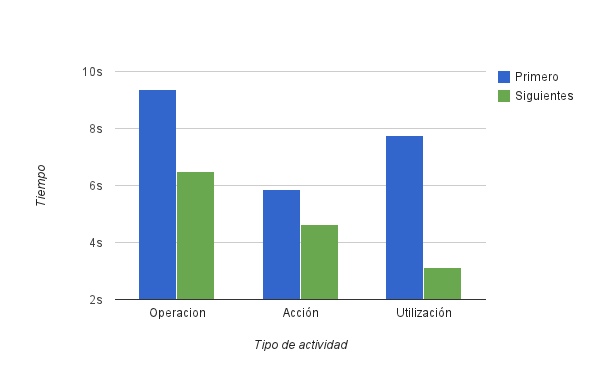
\includegraphics[width=14cm]{resultados/imagenes/interfaz_tiempo_actividades.png}
%\caption{Tiempo por tipo de actividad}
%\label{fig:interfaz_tiempo_acciones}
%\end{figure}

\begin{filecontents}{interfazuso.dat}
n   p       s
1	9.38	6.48
2   5.88	4.64
3   7.75	3.13
\end{filecontents}
\pgfplotstableread{interfazuso.dat}{\InterfazUso}

\begin{figure}[H]
    
        \centering
        \begin{tikzpicture}[scale=1]
           \begin{axis}[ybar,%
              legend pos=outer north east,
              xmin=1,
              xmax=3,
              x=2.5cm,
              enlarge x limits={abs=1cm},
              xtick=data,
              symbolic x coords={0,1,2,3,4},
              ymin=0,ymax=10,
              %ytick={0,2,4,6,8,10},
              xticklabels={Contextual,Interfaz,Herramienta},
              ylabel= Tiempo (s),
              xlabel= Tipo de acción,
              bar width=10pt,
              %enlarge x limits={abs=2},
                ]   
        \addplot[color=blue,ybar,fill=blue!75,area legend] table [x = {n}, y = {p}] {\InterfazUso};
        \addlegendentry{Primer}
        \addplot[color=red,ybar,fill=red!75,area legend] table [x = {n}, y = {s}]
        {\InterfazUso};
        \addlegendentry[align=left]{Promedio \\ siguientes}
        \end{axis}
        \end{tikzpicture}
        \caption{Tiempo por tipo de acción}
        \label{fig:interfaz_tiempo_acciones}
\end{figure}

En la tabla~\ref{tab:interfaz_cantidad_espaciales} se observa la cantidad de
movimientos espaciales realizados por los usuarios, se observa que en promedio
se desplazaron $10,88$ veces por el escenario, y $6,75$ veces acercaron o
alejaron la cámara del paciente.

%\observacion{Hay que dejar bien en claro de donde sale esto, por que es
%importante entender el significado de esta diferencia}

\begin{table}[H]
\centering
\begin{tabular}{lrrr}
\toprule
\textbf{Jugador}  & \textbf{Desplazamiento} & \textbf{Acercamiento/alejamiento} & \textbf{Total} \\
\midrule
1        & 18         & 2    & 20 \\
2        & 7          & 8    & 15 \\
3        & 14         & 12   & 26 \\
4        & 9          & 14   & 23 \\
5        & 5          & 8    & 13 \\
6        & 14         & 4    & 18 \\
7        & 16         & 3    & 19 \\
8        & 4          & 3    &  7 \\
\midrule
\textbf{Promedio} & \textbf{10,88}      & \textbf{6,75} & \textbf{17,63} \\
\bottomrule
\end{tabular}
\caption{Cantidad de movimientos espaciales}
\label{tab:interfaz_cantidad_espaciales}
\end{table}

No existe una cantidad mínima o máxima de movimientos que el usuario debe realizar para acercar, 
alejar o desplazar la cámara. Los datos mostrados en la tabla~\ref{tab:interfaz_cantidad_espaciales} 
muestran que no son necesarias demasiados movimientos. Teniendo en cuenta esta información y la 
proveída en la tabla~\ref{tab:interfaz_tiempo_total}, se concluye 
que en promedio los usuarios realizan $1,7$ movimientos por minuto.

\begin{table}[!hbt]
\centering
\begin{tabular}{lrrr}
\toprule
\textbf{Alumno} & \textbf{Tiempo (min)} \\
\midrule
1        & 8:32 \\
2        & 6:03 \\
3        & 8:33 \\
4        & 5:17 \\
5        & 6:55 \\
6        & 8:40 \\
7        & 7:03 \\
8        & 10:27 \\
\midrule
\textbf{Promedio} & \textbf{7:41} \\
\bottomrule
\end{tabular}
\caption{Tiempo de prueba por usuario}
\label{tab:interfaz_tiempo_total}
\end{table}

El tiempo total que se observa en la tabla~\ref{tab:interfaz_tiempo_total},
muestra que en promedio a cada alumno le tomo $7:41$ minutos realizar todos los
pasos especificados, es importante notar que este tiempo incluye el tiempo de
adaptación. 

La tabla~\ref{tab:interfaz_acciones} nos muestra la cantidad de pasos
realizados por los alumnos de un total de 19. Se observa que en promedio 
realizaron $16.75$ pasos.
%esto permite identificar en que parte del procedimiento los usuarios tienen
%inconvenientes en cuanto al uso de la interfaz.

\begin{table}[H]
\centering
\begin{tabular}{lrrr}
\toprule
\textbf{Alumno} & \textbf{Pasos realizados (19)} \\
\midrule
1 & 19 \\
2 & 15 \\
3 & 18 \\
4 & 15 \\
5 & 18 \\
6 & 16 \\
7 & 19 \\
8 & 14 \\
\midrule
\textbf{Promedio} & \textbf{16,75} \\
\bottomrule
\end{tabular}
\caption{Pasos realizados por alumno}
\label{tab:interfaz_acciones}
\end{table}



\subsubsection{Encuesta}


La encuesta es utilizada para obtener el grado de
disconformidad de los usuarios con respecto a la solución. Se utiliza la disconformidad 
para resaltar los puntos débiles, así, aquellas variables que tengan el mayor porcentaje serán
las que deban ser mejoradas.

%Las preguntas que forman parte de la  encuesta son agrupadas en cuanto a
%aspectos de calidad gráfica, interacción con el entorno, interacción con los
%objetos, características del entorno, usabilidad de la interfaz e integración
%con el hardware.

En la tabla~\ref{tab:interfaz_disconformidad_metrica} se observan que las mayores 
disconformidades son la usabilidad de la interfaz de usuario que llega al $51\%$, la 
interacción de los usuarios con el entorno que llega al $50\%$ y la interacción con los 
objetos que llega al $49\%$. Otras disconformidades con menor porcentaje son las
características del entorno con un  $33\%$, la integración con el hardware con
un $27\%$ y por último la calidad gráfica con un $17\%$.

%\observacion{Hay que explicar que estas pruebas se hicieron de forma previa a
%las demás y que se arreglan algunos casos}

\begin{table}[H]
\centering
\begin{tabular}{lr}
\toprule
Variable & Disconformidad (0-1)\\
\midrule
Calidad Gráfica         & 0.17 \\
Interacción Entorno     & 0.50\\
Interacción Objetos     & 0.49\\
Características Entorno & 0.33\\
Usabililidad Interfaz   & 0.51\\
Integración Hardware    & 0.27\\
\bottomrule
\end{tabular}
\caption{Disconformidad por variable}
\label{tab:interfaz_disconformidad_metrica}
\end{table}

%La conclusión de esta prueba de interfaz, es que si bien, pudo ser utilizada sin
%mayores inconvenientes, existe un alto grado de disconformidad con la interfaz,
%además cabe resaltar, los sujetos de prueba son personas acostumbradas al uso de
%tecnologías similares. Otros puntos débiles encontrados en esta prueba son la
%interacción con el entorno y  con los objetos.

Como consecuencia de los resultados obtenidos, la usabilidad de interfaz y la interacción con objetos y 
con el entorno son mejoradas para obtener la versión final de la solución que es utilizada por 
los estudiantes de enfermería. Las demás pruebas mencionadas en este capítulo son realizadas con 
la versión final de la solución.
%elementos sufren modificaciones a fin de su utilización con usuarios no
%técnicos.

%Las demás pruebas mencionadas en este capítulo son realizadas con la versión
%final de la solución, la cual es obtenida luego de las mejoras realizadas a los
%puntos débiles detectados por esta prueba.

%! TEX root = ../main.tex

\section{Encuesta de ubicación}
\label{sec:ubicacion}

Para recabar información acerca del nivel de acceso  de los alumnos a la
tecnología, se realiza una encuesta que cuenta con diez preguntas, las cuales
buscan conocer el modelo de dispositivo móvil, el acceso a
Internet, y la predisposición de cada alumno a ayudar en la prueba.

Con los resultados de la encuesta de ubicación tecnológica, se seleccionan
aquellos alumnos que poseen dispositivos móviles que superan o igualan las
especificaciones descritas más adelante. De esta encuesta se obtendrán los 
usuarios que formarán parte de la población que evaluará la versión final de 
la solución.

\subsection{Muestra}

En el año $2014$, el \Gls{iab} cuenta con $124$ alumnos en el cuarto año  de la 
carrera de Licenciatura en Enfermería distribuidos en
tres secciones, estos alumnos son considerados la población objetivo. De los 124, 93 de
ellos estuvieron interesados en completar la encuesta.

\subsection{Variables}

Se definen $3$ factores necesarios para que un alumno pueda ser considerado como
sujeto de prueba, el primero es la predisposición del mismo a participar de la
prueba, el segundo es que posea un dispositivo móvil que supere los requisitos
mínimos explicados más adelante y el tercero es que tenga algún tipo de conexión a 
internet desde el dispositivo móvil pues 
los registros de actividad de cada dispositivo deben ser enviados y almacenados 
para su posterior interpretación y análisis. A continuación se describen las variables 
consideradas.


\begin{itemize}

\item \textbf{Requisitos mínimos:} son aquellos requerimientos técnicos con los que 
    debe cumplir completamente el dispositivo móvil del usuario para que la 
    solución tenga un desempeño que garantice una experiencia fluida a la hora de 
    utilizarla. Estos requisitos son:
    \begin{itemize}
        %%\item Sistema Operativo Android $4.0$ o superior
        \item Memoria ram de $512$MB o superior.
        \item Velocidad de procesador de $800$ GHz o superior.
        \item \Gls{gpu} OpenGL ES 2.0 o superior.
        %\item Conexión frecuente a internet.
    \end{itemize}
    Los requisitos de \textit{hardware} mencionados, son requeridos por las
    características de la simulación, una \Gls{gpu} es requerida por los gráficos en 
    tres dimensiones.

\item \textbf{Tipo de acceso a internet:} el tipo de acceso a internet que posee el 
    usuario en su dispositivo móvil. Puede ser una de las siguientes opciones:
    plan post-pago, paquetes pre-pago, acceso ocasional y sin acceso.
    
\item \textbf{Sistema Operativo:} se refiere al tipo de sistema operativo que posee 
    el dispositivo móvil del usuario.

%    \observacion{Donde se menciona?}
    
\end{itemize}

\subsection{Métricas}

Las métricas utilizadas para estudiar los datos recogidos son sencillas ya que
sólo buscan determinar la población que evaluará la solución, estas métricas son
las siguientes:

\begin{itemize}
\item Porcentaje de encuestados con dispositivos móviles que cumplen y que no cumplen con 
los requisitos mínimos.
\item Porcentaje del tipo de acceso a internet de los encuestados desde sus dispositivos móviles.
\item Porcentaje del tipo de sistema operativo que poseen los dispositivos móviles de los 
encuestados.
\end{itemize}


\subsection{Resultados obtenidos}


%Como se indicó en la sección~\ref{sec:ubicacion}, se agrupa a los
%\fixme{alumnos}{De donde?} encuestados de acuerdo a las características de sus
%dispositivos móviles y del acceso a internet.

%El acceso a internet es un requisito importante, pues para que los mismos puedan
%enviar su progreso y así se registre la utilización de la solución, así, es
%necesario que los usuarios tengan un acceso ocasional a internet. 

En la figura~\ref{fig:ubicacion_acceso_internet} se puede observar que de 93 alumnos 
encuestados, el $94,6\%$ tiene acceso a internet al menos en algún momento y que
solo el $5.4\%$ no tiene acceso a internet en sus dispositivos móviles. Considerando 
sólo estos datos, el $94,6\%$ de los alumnos podría utilizar la solución.

%esto
%permite que tengan acceso a la solución el $94,6\%$ de los alumnos.

%\begin{figure}[H]
%\centering
%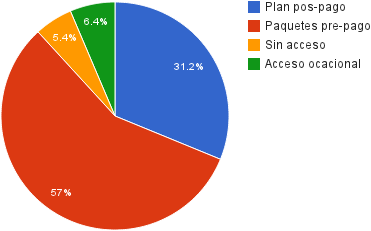
\includegraphics[scale=0.5]{resultados/imagenes/ubicacion_acceso_internet.png}
%\caption{Acceso a internet desde dispositivos móviles}
%\label{fig:ubicacion_acceso_internet}
%\end{figure}

 \begin{figure}[H]
        \centering
        \begin{tikzpicture}[thick,scale=0.7, every node/.style={transform shape}]
            \pie[
                %explode=.2,
                text=legend,
                %style=drop shadow,
                %radius=3,
                %scale font,
                explode={0.1,0.1,0.3,0.3}
                ]%
            {%
                31.2 / Plan pos-pago,
                57   / Paquetes pre-pago,
                5.4  / Sin acceso,
                6.4  / Acceso ocasional}
        \end{tikzpicture}
        \caption{Acceso a internet desde dispositivos móviles}
        \label{fig:ubicacion_acceso_internet}
\end{figure}

%La utilización en dispositivos móviles es un requisito necesario para
%\fixme{la}{Utilizar la solución} solución

Los dispositivos móviles son un requisito para utilizar la solución, 
en la figura\ref{fig:ubicacion_sistemas_operativos} se muestran los sistemas operativos
móviles utilizados por los alumnos encuestados, si bien el motor de videojuego 
utilizado permite generar clientes a diversos sistemas operativos, es importante conocer el sistema
operativo que poseen los alumnos para realizar pruebas.

En la figura~\ref{fig:ubicacion_sistemas_operativos} se puede observar que
\emph{Android} lidera con un $61.3\%$, le sigue Windows Phone con un $12.9\%$.
Si bien, según la tabla~\ref{tab:comparacion_motores_juegos}, \emph{Unity3D}
soporta la mayoría de los sistemas operativos, aún es importante hacer pruebas
sobre un sistema operativo específico. Se selecciona \emph{Android} por ser el
sistema operativo con mayor cuota entre los alumnos.

%\begin{figure}[H]
%\centering
%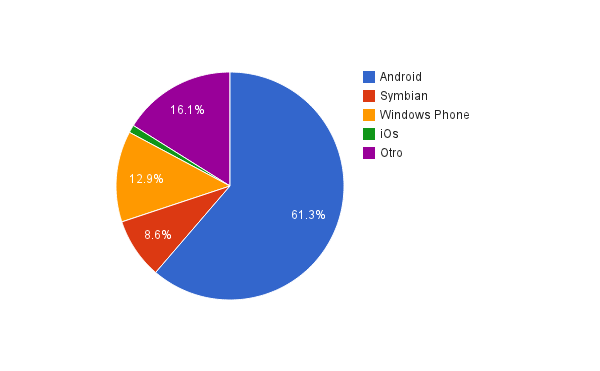
\includegraphics[scale=0.5]{resultados/imagenes/ubicacion_sistemas_operativos.png}
%\caption{Sistemas operativos móviles utilizados}
%\label{fig:ubicacion_sistemas_operativos}
%\end{figure}

 \begin{figure}[H]
        \centering
        \begin{tikzpicture}[thick,scale=0.7, every node/.style={transform shape}]
            \pie[
                text=legend,
                rotate=61.3,
                explode={.1,.2,.2,.2}
                ]%
            {%
            61.3 / Android,
             8.6 / Symbian,
            12.9 / Windows Phone,
            17.2 / Otros}
        \end{tikzpicture}
        \caption{Sistemas operativos móviles utilizados}
	    \label{fig:ubicacion_sistemas_operativos}
\end{figure}
    

Por último, se divide a los encuestados para determinar cuantos de ellos
tiene dispositivos móviles que cumplen los requisitos mínimos para utilizar la
solución propuesta según lo descrito en la sección~\ref{sec:ubicacion}. En la
figura~\ref{fig:ubicacion_requisitos_minimos} se puede observar que el $18,3\%$
de los encuestados cumplen con los requisitos.

Si bien los requisitos de la solución no son elevados para los estándares
actuales, la figura~\ref{fig:ubicacion_requisitos_minimos} nos muestra que el
$18.3\%$ tiene dispositivos de alta gama, el cual es un porcentaje mayor al
esperado. Se observa además que cerca del
$90\%$ posee un dispositivo de gama media o superior, la penetración de los
dispositivos móviles es muy alta en los estudiantes de enfermería del \Gls{iab}.

%\begin{figure}[H]
%\centering
%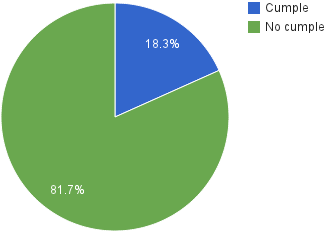
\includegraphics[scale=0.5]{resultados/imagenes/ubicacion_requisitos_minimos.png}
%\caption{Dispositivos que cumplen con los requisitos mínimos para la prueba}
%\label{fig:ubicacion_requisitos_minimos}
%\end{figure}

\begin{figure}[H]
       \centering
       \begin{tikzpicture}[thick,scale=0.7, every node/.style={transform shape}]
           \pie[
                text=legend,
                explode=.1
                ]%
            {%
                81.7 /  No Cumple,
                18.3 /  Cumple
            }
        \end{tikzpicture}
        \caption{Dispositivos que cumplen con los requisitos mínimos para la prueba}
		\label{fig:ubicacion_requisitos_minimos}
\end{figure}

Considerando los datos mostrados, el $17$ alumnos cumplen con los requisitos para utilizar y evaluar 
la solución.




\section{Registro de actividades}
\label{sec:registro}

El registro de actividades ayuda a identificar las  fortalezas y debilidades de
la solución en cuanto al diseño y utilidad. Para que los alumnos puedan formar
una opinión válida acerca de la solución primero deben experimentar con la
misma, para ello se instala la solución en los dispositivos móviles de los
alumnos.

La instalación de la solución se lleva a cabo en el \Gls{iab}, se procede a
mostrar un vídeo de la simulación, explicar la interfaz de usuario y realizar
una muestra de como desenvolverse en el entorno. El período de prueba se
extiende por 20 días, el mismo no es asistido, es decir, existen factores que no
pueden ser controlados, como:

\begin{itemize}
    \item Tiempo dedicado a la simulación por parte del alumno.
    \item Que todas las acciones provengan del alumno.
    \item Que sólo el conocimiento del alumno es puesto a prueba, es decir, no
        se puede controlar que no reciba ayuda externa.
\end{itemize}

Por estos motivos, el uso de la solución propuesta no puede ser considerado el
único factor relacionado con los resultados obtenidos en la \emph{Encuesta para
    medir el conocimiento}, cuyos resultados son mostrados más adelante en la
sección~\ref{sec:objetiva}.

La solución propuesta almacena información relacionada a la actividad del
usuario, incluyendo cuándo y cómo realiza las acciones, los pasos que realiza,
el orden y las condiciones de la escena cuando realiza cada acción.

El registro como un todo es enviado cada vez que el usuario desee, este envío
requiere una conexión a internet, por ello no es automático. Adicionalmente el
último día de la prueba, todos los registros fueron enviados para que sean
analizados.

\subsection{Muestra}

La muestra está conformada por los $11$ alumnos que aceptaron formar parte de 
la prueba y poseen dispositivos móviles que cumplen con los requisitos
mínimos descritos en la sección~\ref{sec:ubicacion}.

La utilización de $11$ alumnos es suficiente, ya que según estudios presentados
en~\cite{nielsen2000}, mientras menos experiencia tengan los sujetos de estudio
con la solución planteada, serán necesarios menos para detectar un gran
porcentaje de errores y fortalezas, y según~\cite{ritch2009}, una base de $10$ a
$12$ es suficiente para obtener resultados estadísticamente válidos.

\subsection{Variables}

%La utilización de la solución, y el registro de las actividades genera una
%gran cantidad de información, los factores que se desean medir están
%relacionados a aquellos que pueden ser contrastados con los resultados de la
%encuesta objetiva.

Los registros de actividades nos permiten obtener información relevante acerca
de cómo se utilizó la solución y cuál fue el desempeño de los usuarios, las variables a medir son 
las siguientes:


\begin{description}

\item[Cantidad de partidas:] se define como el número de veces que un usuario
    inicia una escena. 

\item[Tiempo total:] es la suma del tiempo empleado en todas las partidas.

\item[Tiempo total de partidas por usuario y por tipo:] es el tiempo total 
    empleado para jugar las partidas discriminadas por tipo y por usuario.

\item[Cantidad de acciones:] es la cantidad total de acciones realizadas por 
    los usuarios.
 
\item[Cantidad de partidas realizadas por usuario y por tipo:] es el número de 
    partidas jugadas por usuario discriminado por el procedimiento al que 
    corresponde.

\item[Cantidad de usuarios:] es el número de usuarios que utilizaron la solución.
    
\item[Puntuación de las partidas:] dado el registro de reglas cumplidas en una partida 
    del procedimiento de venopunción o el diagnóstico dado por el usuario 
    en una partida del procedimiento de valoración de la escala de Glasgow, se 
    puede obtener el desempeño del usuario en las partida. 
%    Esto puede ser contrastado 
%    con la puntuación obtenida por el usuario en la \emph{Encuesta Objetiva}.

%\item[Puntuación por regla cumplida] Las variables definidas
%    en~\ref{sec:objetiva}, pueden ser contrastadas con la puntuación obtenida
%    por los alumnos en la simulación.

\end{description}

\subsection{Métricas}

Las métricas utilizadas para el análisis de los registros de actividades son las siguientes:

\begin{description}
\item[Promedio de tiempo por partida:] se obtiene dividiendo el tiempo total empleado 
    en las partidas por el número de partidas.
\item[Promedio de acciones por partida:] se obtiene dividiendo la cantidad total de 
    acciones realizas por los usuarios por el número de partidas.
\item[Promedio de partidas por usuario:] se obtiene dividiendo el número total de partidas
    por el número de usuarios que utilizaron la solución.
\item[Total de sesiones jugadas por tipo:] es la suma del número de partidas jugadas por los 
    usuarios discriminadas por tipo.
\item[Total de tiempo jugado por tipo:] es la suma de la cantidad de tiempo empleado en una 
    partida por los usuarios discriminado por tipo.
\item[Promedio de siguientes puntajes por tipo y por usuario:] se obtiene dividiendo la suma 
    de los puntajes obtenidos en cada tipo de escenario por la cantidad de veces que jugó el 
    usuario, a excepción de la primera vez.
\end{description}

%Además de las métricas descritas también se utiliza la correlación de Pearson como se 
%explica en \ref{sec:correlacion} para identificar las relaciones entre los datos obtenidos en 
%la \emph{Encuesta Objetiva} y los obtenidos en el \emph{Registro de actividades}.

\subsection{Resultados obtenidos}

%Las actividades de los usuarios son registradas y almacenadas para su análisis, a
%continuación se presentan los resultados de ese análisis, el mismo fue descrito
%en~\ref{sec:registro}, 

En la tabla~\ref{tab:log_total} se observa un resumen del experimento, en cuanto a tiempo, partidas y acciones.


\begin{table}[H]
\centering
\begin{tabular}{lrrrrrrrr}
%\toprule
%\textbf{Variable}                         & \textbf{Valor} \\
\toprule
Partidas                         & 99 \\
Primera partida					 & 4 de noviembre de 2014 \\
Última partida					 & 23 de noviembre de 2014 \\
\midrule
Tiempo total                     & 11134 s \\
Promedio de tiempo por partida   & 112 s \\
\midrule
Acciones                         & 2944 \\
Promedio de acciones por partida & 30 \\
\midrule
Usuarios                         & 8 \\
Promedio de partidas por usuario & 12 \\
\bottomrule
\end{tabular}
\caption{Resumen de la información extraída del registro de actividades}
\label{tab:log_total}
\end{table}

La cantidad de partidas jugadas por usuario en el procedimiento de venopunción, se muestra en la
tabla~\ref{tab:log_hemocultivo_partida}, se observa que existen $3$ alumnos que no
participaron de la prueba o no se registraron sus actividades.

\begin{table}[H]
\centering
\begin{tabular}{lrrrrrrrr}
\toprule
& \multicolumn{2}{c}{Venopunción} \\
\cmidrule(lr){2-3} 
Alumno   & Sesiones jugadas & Tiempo jugado (s) \\
\midrule
 1       & 5                & 1202 \\
 2       & 19               & 2507 \\
 4       & 5                & 398  \\
 5       & 6                & 768  \\
 6       & 17               & 2371 \\
 7       & 7                & 707  \\
 9       & 1                & 126  \\
10       & 8                & 960  \\
\midrule
Total   & 68               & 9039 \\
\bottomrule
\end{tabular}
\caption{Número de partidas y tiempo total por alumno en segundos, en la escena
    de venopunción.}
\label{tab:log_hemocultivo_partida}
\end{table}



Los registros pueden no ser registrados sí
\begin{enumerate*}[label=\itshape\alph*\upshape)]
    \item el usuario utilizó la solución, no envió los datos y, luego
        desinstaló la solución o borró los datos de la misma, o,
    \item el usuario no utilizó la solución.
\end{enumerate*}

En la tabla~\ref{tab:log_glasgow_random_partida}, se observa la cantidad de
sesiones y tiempo total por alumno, en la escena de \textit{Glasgow}, en modo de
evaluación. Se observa que $5$ alumnos participaron en $22$ sesiones, en total
jugaron $1768$ segundos. En cambio, en la tabla~\ref{tab:log_glasgow_custom_partida} se 
observa que $4$ alumnos participaron en $9$ sesiones y en total jugaron $327$ segundos. 
Los alumnos prefirieron jugar en el modo que les permitía diagnosticar al paciente.

\begin{table}[H]
\centering
\begin{tabular}{lrrrrrrrr}
\toprule
& \multicolumn{2}{c}{Glasgow (Evaluación)} \\
                   \cmidrule(lr){2-3} 
Número de alumno   & Sesiones jugadas                            & Tiempo jugado (s) \\
\midrule
1     & 4  & 211 \\
2     & 8  & 738 \\
4     & 3  & 132 \\
6     & 1  & 97  \\
7     & 6  & 590 \\
\midrule
Total & 22 & 1768 \\
\bottomrule
\end{tabular}
\caption{Número de partidas y tiempo total por alumno en segundos, en la escena
    \textit{Glasgow}, en modo evaluación}
\label{tab:log_glasgow_random_partida}
\end{table}


\begin{table}[H]
\centering
\begin{tabular}{lrrrrrrrr}
\toprule
& \multicolumn{2}{c}{Glasgow (Exploración)} \\
                   \cmidrule(lr){2-3} 
Número de alumno   & Sesiones jugadas                            & Tiempo jugado (s) \\
\midrule
1        & 2 & 79 \\
2        & 3 & 80 \\
4        & 3 & 89 \\
6        & 1 & 79 \\
\midrule
Total   & 9 & 327 \\
\bottomrule
\end{tabular}
\caption{Número de partidas y tiempo total por alumno en segundos, en la escena
    \textit{Glasgow}, en modo exploración}
\label{tab:log_glasgow_custom_partida}
\end{table}


En las tablas~\ref{tab:log_hemocultivo_puntaje}
y~\ref{tab:log_glasgow_random_puntaje} se muestran los primeros puntajes y un
promedio de los puntajes siguientes obtenidos por cada alumno en los
procedimientos de venopunción y de la evaluación de la escala de
Glasgow. Se debe tener en cuenta el tiempo y la cantidad de veces que cada
alumno jugó cada uno de los procedimientos para valorar los resultados
mostrados. 

\begin{table}[H]
\centering
\begin{tabular}{lrrrrrrrr}
\toprule
& \multicolumn{2}{c}{Venopunción} \\
\cmidrule(lr){2-3} 
Número de alumno  & Primer Puntaje & Siguientes Puntajes \\
\midrule
 1                & 11             & 14.3 \\
 2                & 9              & 10.6 \\
 4                & 3              & 3.3  \\
 5                & 3              & 6.8  \\
 6                & 3              & 5.8  \\
 7                & 4              & 4    \\
 9                & 16             & \\
10                & 3              & 7.2  \\
\midrule
\textbf{Promedio} & 6.5            & 7.42 \\
\bottomrule
\end{tabular}
\caption{Puntaje obtenido la primera vez y el promedio de los puntajes de las siguientes veces
    por alumno, en la escena de venopunción}
\label{tab:log_hemocultivo_puntaje}
\end{table}


\begin{table}[H]
\centering
\begin{tabular}{lrrrrrrrr}
\toprule
& \multicolumn{2}{c}{Glasgow (Evaluación)} \\
                   \cmidrule(lr){2-3} 
Número de alumno   & Primer Puntaje & Siguientes Puntajes \\
\midrule
1     & 1 & 1.5 \\
2     & 2 & 2.3 \\
4     & 1 & 1.5 \\
6     & 2 & 2 \\
7     & 0 & 1 \\
\midrule
\textbf{Promedio} & 1.2 & 1.66 \\
\bottomrule
\end{tabular}
\caption{Puntaje obtenido la primera vez y el promedio de los puntajes de las siguientes veces
    por alumno, en la escena \textit{Glasgow}, en modo evaluación}
\label{tab:log_glasgow_random_puntaje}
\end{table}

En las tablas~\ref{tab:log_hemocultivo_puntaje}
y~\ref{tab:log_glasgow_random_puntaje} se observa que los alumnos que participaron de la prueba
mejoran su desempeño a medida que aumenta el número de partidas. 

%Es importante notar que la cantidad de partidas no es uniforme entre los
%alumnos, es decir hay alumnos con más de $10$ partidas y alumnos con menos de
%$5$, por ello, no es posible demostrar que existe un progreso a medida que
%aumenta el número de partidas.

Por último, en la figura~\ref{fig:utilizacion_hora} se puede observar la distribución de 
las partidas por hora del día. Los picos de uso de la solución se dan a las $13:00$ horas, 
horario de almuerzo, a las $17:00$ horas, fin de las actividades académicas y a las $01:00$ horas, 
horario libre. De esta manera los datos muestran que el mayor uso de la solución se da en los 
horarios libres de los alumnos, es decir, los alumnos deciden usar la solución en su tiempo libre.

\begin{filecontents}{utilizaciontiempo.dat}
Hora	Cantidad
 0	 0
 1	 9
 2	 4
 3	 2
 4	 0
 5	11
 6	 8
 7	 3
 8	 5
 9	 7
10	 7
11	12
12	15
13	 9
14	 6
15	 0
16	 0
17	 0
18	 0
19	 0
20	 0
21	 0
22	 0
23	 1
24	 0
\end{filecontents}
\pgfplotstableread{utilizaciontiempo.dat}{\UtilizacionTiempo}

\begin{figure}[H]
	\centering
    \begin{tikzpicture}[thick, scale=1.2]
        \begin{axis}[
            title={},
            xlabel={Hora},
            ylabel={Partidas},
            xmin=0, xmax=24,
            ymin=0, ymax=16,
            xtick       = {0  , 3  , 6  , 9  , 12 , 15 , 18 , 21 , 24},
            xticklabels = {12 , 15 , 18 , 21 ,  0 , 3  ,  6 ,  9 , 12},
            %ytick={0,.25,.50,.75,1},
            legend pos=north east,
            ymajorgrids=true,
            xmajorgrids=true,
            grid style=dashed,
        ]
         
        \addplot[color=blue,fill=blue!5] table [x = {Hora}, y = {Cantidad}] {\UtilizacionTiempo};
        \end{axis}
    \end{tikzpicture}
    \caption{Utilización de la solución por hora del día}
    \label{fig:utilizacion_hora}
\end{figure}

%! TEX root = ../main.tex
\section{Encuesta Subjetiva}

En el análisis de los resultados, existieron alumnos que no respondieron todas
las preguntas, para tratar este tipo de casos, es importante analizar la
naturaleza del patrón de datos faltantes\cite{carpita2011imputation}. Existen
tres posibles formas de categorizar el patrón de ocurrencia de falta de
respuestas\cite{leite2010performance}\cite{leite2010performance}\cite{tsikriktsis2005review}:


\begin{description}
    \item[Información faltante completamente aleatoria] Cuando la información
        faltante es independiente de la variable medida y de otras variables.
    \item[Información faltante aleatoria] Cuando la información faltante depende
        de otras variables, pero no de la variable en sí. 
    \item[Información faltante no aleatoria] Cuando hay una relación entre la
        información faltante y el valor de la variable.
\end{description}

Los datos muestran que la información faltante es completamente aleatoria en
relación a la variable medida y a las demás variables, de hecho, una sola
encuesta tiene información faltante, así, se establece que el tipo de
información faltante es \emph{Información faltante completamente aleatoria}.

Existen tres mecanismos\cite{tsikriktsis2005review} principales para lidiar con
información faltante, eliminación, reemplazo, y procedimientos basados en modelo
(?Model-based procedure XXX).\cite{tsikriktsis2005review} recomienda utilizar
un mecanismo de reemplazo para escalas del tipo Likert.

Las técnicas de reemplazo se clasifican en tres grandes
grupos\cite{tsikriktsis2005review}:
\begin{enumerate*}[label=\itshape\alph*\upshape.]
\item basadas en la promedio,
\item basadas en regresión, y,
\item imputación \emph{hot deck}.
\end{enumerate*}

La sustitución basada por promedio, se divide nuevamente en tres grupos;
promedio
\begin{enumerate*}[label=\itshape\alph*\upshape.]
\item total,
\item del subgrupo, y,
\item por caso.
\end{enumerate*}
La sustitución del promedio total se realiza obteniendo el promedio de todas las
respuestas de esta pregunta, la sustitución de subgrupo es similar, solo que se
limita a aquellos sujetos del mismo subgrupo del sujeto que no respondió, y
finalmente, la sustitución por caso, es el promedio de las respuestas válidas
del sujeto.

En su resumen de las diferentes técnicas y cuando se deben utilizar cada una,
\cite{tsikriktsis2005review}, recomienda la utilización de la sustitución basada
en promedio por caso. 

De esta forma se reemplazan los valores faltantes en la encuesta, con el
promedio del sujeto.

%! TEX root = ../main.tex

\section{Encuesta para evaluar el conocimiento}
\label{sec:objetiva}

A fin de obtener información acerca del conocimiento de los alumnos  que forman parte de la 
población objetivo, es decir, aquellos que utilizaron 
la solución propuesta y los que no la utilizaron, los cuales constituyen el grupo 
de control, se realiza una encuesta que consta de diez preguntas.

La encuesta mide el nivel de conocimiento del alumno sobre los dos temas
simulados, contiene preguntas de nivel básico, medio y avanzado. Las mismas son
formuladas utilizando la lista de competencias básicas que debe tener un alumno
para aprobar la materia \textbf{Enfermería en Urgencias II}. Las preguntas son
verificadas  por los profesores de la cátedra. Cada pregunta tiene el mismo
peso, así la puntuación más baja obtenible es $0$, y la más alta es $10$.

De esta manera se busca evaluar la influencia pedagógica de la 
solución como herramienta de apoyo al aprendizaje.


\subsection{Muestra}
%\observacion{Se repite mucho lo de las muestras hay 2 universos nomas?}

La población objetivo cuenta con $124$ alumnos, de los cuales $11$ son la muestra seleccionada
para la prueba de la solución, y los $113$ alumnos restantes son utilizados
como grupo de control.

\subsection{Variables}

Se busca medir el puntaje total de los alumnos en la \emph{Encuesta para evaluar el conocimiento}. Esto 
se obtiene de la siguiente manera.

Siendo:

\begin{itemize}
    \item $po_i{_k}$ la respuesta del usuario $i$ a la pregunta $k$
    \item $n$ total de preguntas, igual a 10
    \item $tc$ total de alumnos en el grupo de control, igual a 113.
    \item $t$ total de alumnos, igual a 124
    \item $ts$ total de sujetos de estudio, igual a 11.
\end{itemize}

Se define el puntaje total $pto_i$ del alumno $i$ como, 

\begin{equation*}
    pto_i = \sum_{j=1}^n{po_i{_j}}
\end{equation*}


\subsection{Métricas}

Como se mencionó, la \emph{Encuesta para evaluar el conocimiento} busca medir el rendimiento de los 
alumnos, para ello se utiliza como métrica principal el promedio de acierto, 
tanto del conjunto total de alumnos de la población objetivo, como de los que participaron de la
prueba, y del grupo de control por separado.

Se define el promedio total de los alumnos, $promtotal$ como:

\begin{equation*}
    promtotal = \frac{\sum_{i=1}^t{pto_i}}{t}
\end{equation*}

Se obtienen los promedios del grupo de control ($promcontrol$) y del grupo de alumno que
participo en la prueba para evaluar la solución ($promsujetos$) de la misma manera.

\subsection{Resultados obtenidos}
\label{sec:res_objetiva}

Como se detalló en la sección~\ref{sec:objetiva}, la encuesta realizada a cada
usuario, parte de la prueba, es utilizada para obtener una comparación en cuanto
al rendimiento de los usuarios que forman parte de la muestra y los que forman
parte del grupo de control.


%\observacion{A esta altura ya no se entiende que es promcontrol}
%\observacion{No estaría mal poner algún tipo de información que diga a que
%aspectos se relacionad cada pregunta}

La tabla~\ref{tab:objetiva_rendimiento_por_pregunta} muestra el nivel de acierto
en promedio por pregunta de los usuarios que forman parte de la muestra y de los
que forman parte del grupo de contro. Según estos datos, en el $60\%$ de los casos 
hay una leve mejoría en cuanto al nivel de acierto para los usuarios que forman 
parte de la muestra.

\begin{table}[H]
\centering
\begin{tabular}{lrrr}
\toprule
& \multicolumn{3}{c}{Promedio} \\
\cmidrule(lr){2-4}
\textbf{Pregunta} & 
\textbf{Muestra} & 
\textbf{Grupo Control} & 
\textbf{Total} \\ 
\midrule
ES1. Torniquete           & 0.36 & 0.18 & 0.20 \\
ES2. Guantes              & 0.64 & 0.60 & 0.60 \\
ES3. Manos                & 0.09 & 0.14 & 0.13 \\
ES4. Bioseguridad         & 0.27 & 0.25 & 0.26 \\
ES5. Explicación          & 0.82 & 0.56 & 0.59 \\
\midrule
EG1. Diagnóstico Global 1 & 0.00 & 0.18 & 0.16 \\
EG2. Diagnóstico Global 2 & 0.64 & 0.51 & 0.53 \\
EG3. Respuesta ocular     & 0.45 & 0.28 & 0.29 \\
EG4. Respuesta motora     & 0.18 & 0.32 & 0.31 \\
EG5. Respuesta verbal     & 0.36 & 0.45 & 0.45 \\
\midrule
\textbf{Sumatoria}: & 3.82 & 3.47 & 3.49  \\
\bottomrule
\end{tabular}
\caption{Rendimiento promedio de usuarios por pregunta}
\label{tab:objetiva_rendimiento_por_pregunta}
\end{table}

Los datos sólo sugieren levemente una tendencia a la mejoría de los puntajes
para los usuarios que forman parte de la muestra, sin embargo, estos datos no
pueden ser tomados para realizar conclusiones ya que la cantidad de sesiones de
juego por usuario no se considera suficiente para que el uso de la solución
propuesta afecte realmente en el aprendizaje del usuario. Cabe destacar, que 
tanto la muestra como el grupo de control respondieron a la encuesta luego del examen 
final de la materia \emph{Enfermería en Urgencias II}, la cual requería el dominio de ambos 
temas simulados.

\section{Correlación entre variables}
\label{sec:correlacion}

En la tabla~\ref{tab:all_correlation} se observa la correlación entre cinco
variables estudiadas, a fin de observar si existe alguna correlación entre los
valores, se utiliza la correlación de \emph{Pearson}, descrita
en~\ref{sec:correlacion}.

\begin{table}[H]
\centering
\begin{tabular}{lrrrrrr}
\toprule
        &
\begin{sideways}\textbf{Tiempo de Uso}\end{sideways}             &
\begin{sideways}\textbf{Encuesta solución}\end{sideways}        &
\begin{sideways}\textbf{Encuesta conocimiento}\end{sideways}         &
\begin{sideways}\textbf{Puntaje Máximo Extracción}\end{sideways} &
\begin{sideways}\textbf{Puntaje Máximo Glasgow}\end{sideways}    \\
\midrule
Tiempo de Uso             & 1    & -0.2  & 0.15  & 0.62 & 0.41 & 0.78 \\
Encuesta solución         & -0.2 & 1     & -0.07 & 0.04 & 0.11 & -0.28\\
Encuesta conocimiento     & 0.15 & -0.07 & 1     & 0.44 & 0.44 & 0.02 \\
Puntaje máximo Extracción & 0.62 & 0.04  & 0.44  & 1    & 0.96 & 0.44 \\
Puntaje máximo Glasgow    & 0.41 & 0.11  & 0.44  & 0.96 & 1    & 0.27 \\
\bottomrule               & 0.78 & -0.28 & 0.02  & 0.44 & 0.27 & 1    \\
\end{tabular}
\caption{Correlación entre factores estudiados} 
\label{tab:all_correlation}
\end{table}

Las correlaciones fuertes, que se observan en la
tabla~\ref{tab:all_correlation}, son:

\begin{itemize}
    \item Tiempo de uso y puntaje máximo extracción, $0,62$, correlación
        positiva fuerte.
    \item Tiempo de uso y puntaje máximo Glasgow, $0,78$, correlación positiva
        muy fuerte.
    \item Puntaje máximo extracción y encuesta objetiva, $0,44$, correlación
        positiva fuerte.
\end{itemize}


La tabla~\ref{tab:all_correlation} indica que existe una correlación positiva
fuerte ($0,62$ y $0,78$) entre el tiempo de uso y el puntaje más alto obtenido,
\fixme{lo que sugiere que mientras más se utiliza la solución, se obtienen mejores
resultados}{Guardaaaa correlación no es igual que casualidad}. 

Una correlación positiva fuerte entre el puntaje máximo obtenido en la
Extracción y la encuesta objetiva ($0,44$), sugiere que existe una relación entre
el nivel de conocimientos de los alumnos y su desempeño en la práctica.


\chapter{Evaluación}

Dada la propuesta de solución, en este capítulo se proponen mecanismos para medir la
efectividad de la misma.

La evaluación está orientada a la validación de las hipótesis planteadas durante
el desarrollo de la solución, específicamente relacionados a aspectos
pedagógicos, de utilidad y de la participación activa del usuario. Como parte de la 
evaluación se miden ciertas variables relacionadas a los aspectos mencionados.

Este capítulo describe como fueron evaluados los principales aspectos que fueron
tenidos en cuenta en el desarrollo de la solución. Los temas abordados son los siguientes:
objetivos, variables, metodologías y métrica. En cada sección se van detallando
lo que abarca cada punto mencionado.


Para la obtención de la información deseada acerca de la utilización de la
solución y de su impacto en el aprendizaje, se utilizan tres mecanismos que en
conjunto nos ayudan a responder a los objetivos de la evaluación.

La evaluación se divide en tres partes, una encuesta subjetiva que pretende
obtener información acerca de la satisfacción de los usuarios, de ahora en
adelante \textbf{encuesta subjetiva}, un examen que mide los factores
relacionados al aprendizaje, de ahora en adelante \textbf{encuesta objetiva}  y
finalmente una evaluación del registro de actividad de cada jugador que es
registrado automáticamente por la solución.


Se realizaron cuatro evaluaciones a la solución, la primera fue con personas
no relacionadas con el área de enfermería, y las siguientes tres con alumnos del
4to año de Licenciatura en enfermería del \Gls{iab}.

\section{Objetivos}
\label{sec:objetivos}

Las registros de actividad y encuesta objetiva buscan obtener información sobre
el aprendizaje y la utilización de la solución, mientras que la encuesta
subjetiva busca obtener información acerca de las fortalezas y debilidades de
una simulación para el entrenamiento de enfermeros y de la solución propuesta.

Se definen los objetivos principales de la evaluación como siguen:

\begin{itemize}

\item Validar las hipótesis asumidas durante el desarrollo de la
    solución\martin{Se debe hacer referencia a una sección de la propuesta donde
        se hacen las hipótesis?}.

\item Proponer criterios que puedan utilizarse para la evaluación de
    soluciones similares.

\item Evaluar los puntos fuertes y débiles de la solución en cuanto a los
    criterios definidos.

\item Determinar los factores que afectan al uso de herramientas similares para
    apoyo a profesionales de enfermería.

\item Determinar el nivel de aceptación de herramientas alternativas para el
    aprendizaje.

\item Determinar que factores de la solución propuesta motivan a la utilización
    de soluciones similares.

\end{itemize}






%Ideas tipo tiro al aire de La princesa de cocho por si sirvan
%Para la evaluacion acerca de la validez de las hipotesis planteadas en este trabajo se hacen uso de metodologias como registros de actividades de los usuarios cuando utilizan la aplicacion y encuestas para valorar la opinion de los mismos sobre las caracteristicas de la aplicacion.

%Los objetivos principales de la evaluacion son los siguientes:

%* Verificar la validez de las hipotesis planteadas en el desarrollo de la solucion.
%* Proponer criterios que puedan utilizarse para la evaluacion de aplicaciones de esta naturaleza.
%* Obtener conclusiones acerca de factores externos que afectan el uso de la aplicacion.
%* Identificar los puntos importantes en los que se debe poner enfasis en el desarrollo de las aplicaciones con esta naturaleza.
%* Obtener sugerencias de las correlaciones entre el registro de actividades y el examenen de conocimientos realizado a los usuarios de la aplicacion.
%* Obtener conclusiones generales acerca del uso de la aplicacion como herramienta de apoyo al aprendizaje de estudiantes de enfermeria.










\section{Interfaz de usuario}

La primera fue realizada con alumnos de la carrera de Ingeniería en Informática
de la Facultad Politécnica que pertenece a la Universidad Nacional de Asunción,
sin experiencia previa tanto con la solución como con los procedimientos
simulados, pero si familizarizados con la utilización de dispositivos móviles.

\cite{nielsen2000} recomienda una muestra de 5 personas para pruebas de
usabilidad.~\cite{ritch2009} menciona que con 5 individuos, se encuentran 85\%
de los errores en promedio, y que un grupo de 5 a 10 personas es adecuado para
pruebas de usabilidad sencillas.

Esta prueba no es de gran complejidad, el procedimiento es sencillo y esta
bien definido, se busca determinar que problemas presenta la interfaz, que
impedimentos encuentran usuarios acostumbrados a la tecnología pero no al
procedimiento, por ello se elige una muestra de 8 alumnos.

\subsection{Muestra}

La primera fue realizada con alumnos de la carrera de Ingeniería en Informática
de la Facultad Politécnica que pertenece a la Universidad Nacional de Asunción,
sin experiencia previa tanto con la solución como con los procedimientos
simulados, pero si familizarizados con la utilización de dispositivos móviles.

\cite{nielsen2000} recomienda una muestra de 5 personas para pruebas de
usabilidad.~\cite{ritch2009} menciona que con 5 individuos, se encuentran 85\%
de los errores en promedio, y que un grupo de 5 a 10 personas es adecuado para
pruebas de usabilidad sencillas.

Esta prueba no es de gran complejidad, el procedimiento es sencillo y esta
bien definido, se busca determinar que problemas presenta la interfaz, que
impedimentos encuentran usuarios acostumbrados a la tecnología pero no al
procedimiento, por ello se elige una muestra de 8 alumnos.

%! TEX root = ../main.tex

\section{Encuesta de ubicación}
\label{sec:ubicacion}

\observacion{No repitan (se refiere al obtener información)}

A fin de obtener información acerca del nivel de acceso  de los alumnos a la
tecnología, se realiza una encuesta que cuenta con diez preguntas, las cuales
buscan obtener información acerca del modelo de dispositivo móvil, el acceso a
Internet, y la predisposición de cada alumno a ayudar en el experimento.

En el año $2014$, el \Gls{iab} cuenta con $124$ alumnos en el cuarto año distribuidos en
tres secciones, el cual es considerado el Universo. De los 124, 93 de
ellos estuvieron dispuestos a participar de la prueba y completaron la encuesta.

Con los resultados de la encuesta de ubicación tecnológica, se seleccionan
aquellos alumnos que posean dispositivos móviles que superan o igualan las
especificaciones.


\subsection{Variables}

Se definen $2$ factores necesarios para que un alumno pueda ser considerado como
sujeto de experimento\revisar{Utilizar termino prueba}, el primero es la
predisposición del mismo a participar del experimento y el segundo es que posea
un dispositivo móvil que supere los requisitos mínimos.

Los requisitos mínimos para que la solución tenga un desempeño que garantice una
experiencia fluida a la hora de utilizarla son:

\begin{itemize}
    \item Sistema Operativo Android $4.0$ o superior
    \item Memoria ram de $512$MB o superior.
    \item Velocidad de procesador de $800$ GHz o superior.
    \item \Gls{gpu} Mali 400 o superior.
    \item Conexión frecuente a internet.
\end{itemize}

El conjunto de funcionalidades utilizadas por la solución requiere un \Gls{api}
Android de nivel 14\cite{android:api} o superior, lo cual corresponde a un
sistema operativo Android 4.0.

Los requisitos de \textit{hardware} mencionados, son requeridos por las
características de la simulación, y la plataforma utilizada, es requerida una
\Gls{gpu} por los gráficos en tres dimensiones.

La conexión a Internet es requerida, pues los registros de actividad de cada
dispositivo deben ser enviados y almacenados para su posterior interpretación y
análisis.

\section{Encuesta objetiva}
\label{sec:objetiva}

A fin de obtener información comparativa acerca del conocimiento de los alumnos
que utilizaron la aplicación y los que no la utilizaban, utilizados como un
grupo de control, se realizo un examen, que consta de diez preguntas.

El examen busca medir el nivel de conocimiento del alumno sobre los dos temas
simulados, contiene preguntas de nivel básico, medio y avanzado.

Las preguntas fueron formuladas utilizando la lista de competencias básicas que
debe tener un alumno para aprobar la materia \textbf{Enfermería en Urgencias
    II}, y posteriormente fueron aprobadas por los profesores de la cátedra.

Cada pregunta tiene el mismo peso, así la puntuación más baja obtenible es 0, y
la más alta es 10.

\section{Muestra}

El universo cuenta con 124 alumnos, de los cuales 11 son la muestra seleccionada
para el experimento, entonces se utilizan a los 113 alumnos restantes como un 
grupo de control.

\section{Encuesta subjetiva}
\label{sec:subjetiva}

Al final del periodo de prueba, cada alumno de la muestra completa una encuesta
con 31 preguntas que se utilizan para validar las hipótesis. Las preguntas están
agrupadas en dos, el primer grupo cuenta con 27 preguntas cerradas, es decir de
una sola respuesta en una lista de opciones, el segundo grupo cuenta con 4
preguntas abiertas. 

Cada encuesta es entregada a los alumnos que acordaron participar en el
experimento, mientras completan la encuesta, un guía está presente para
responder cualquier duda.

La métrica utilizada es la escala de Likert, descrita en la
sección~\ref{sec:likert}.

\subsection{Variables}
\label{sec:variables}

De acuerdo a los objetivos planteados en la sección~\ref{sec:objetivos}, se
busca describir los factores analizados en las pruebas y las variables
relacionadas a los mismos, las cuales, tienen por objetivo demostrar la validez
de las hipótesis planteadas en este trabajo.

Las variables se presentaran agrupadas en factores, los mismos representan
aquellos aspectos de la solución propuesta que buscan ser evaluados.

\subsubsection{Exploración}
\label{sec:sub_exploracion}

Este factor esta relacionado con la característica que posee la solución en
cuanto a la oportunidad que brinda al usuario para explorar cada uno de los
elementos del entorno simulado (paciente, herramientas propias del
procedimiento). En este sentido, se busca proveer facilidad de uso, intuitividad
y realismo en cuanto a las acciones y situaciones que se presentan en la
solución para que de esta manera, los elementos que la componen no representen
para el jugador un obstáculo que impida su uso.

Las variables que miden este aspecto son las siguientes:

\begin{description}

\item[Funciones realizadas por los elementos del juego] se refiere a la
    correctitud con la que una herramienta o elemento del juego representa las
    funciones que el mismo puede realizar en la vida real, en este sentido, se
    evalúa el realismo con el que es representado tal elemento.

\item[Aleatoriedad para afianzar conocimientos] se refiere al beneficio que
    puede traer el hecho de que el estado del paciente en el juego sea aleatorio
    en cuanto a la posibilidad que esto brinda al jugador para poner a prueba
    sus conocimientos teóricos.

\item[Aleatoriedad para representar realismo] se refiere al uso de estados
    aleatorios en el paciente para que de esta forma el procedimiento se asemeje
    mas a una situación real.

\item[Facilidad de uso] se refiere a lo fácil e intuitivo  que puede ser la
    utilización de los elementos del juego.

\end{description}

\subsubsection{Representación}
\label{sec:sub_representacion}

Este factor esta relacionado con la calidad y suficiencia con la que se
representan los diferentes objetos que son simulados en la solución. La
representación abarca tanto funcionalidad como aspecto del objeto.

De esta manera, se busca permitir al jugador realizar con los objetos las
acciones que requiera para llevar a cabo el procedimiento que se le presente en
la solución, y además, representar estos elementos de la mejor manera posible,
de forma realista.

Las variables que miden estos aspectos son las siguientes:

\begin{description}

\item [Movimientos motrices del paciente] se refiere a la suficiencia de los
    movimientos motrices que realiza el paciente en el escena correspondiente a
    la valoración de la escala de Glasgow.

\item [Movimientos oculares del paciente] se refiere a la suficiencia de los
    movimientos oculares que realiza el paciente en la escena correspondiente a
    la valoración del escala de Glasgow.

\item [Reacción verbal del paciente] se refiere a la suficiencia de las
    reacciones o respuestas verbales que realiza el paciente en la escena
    correspondiente a la valoración de la escala de Glasgow.

\item[Distinción entre los estados del paciente] se refiere a si los diferentes
    estados del paciente son distinguidos correctamente en el procedimiento de
    valoración de la Escala de Glasgow ya que esto es importante para que el
    jugador pueda diagnosticar correctamente al paciente.

\item[Acciones las herramientas] se refiere a si las diferentes acciones que
    pueden realizarse con los elementos o herramientas del juego en un
    determinado procedimiento de enfermería son suficientes para ese
    procedimiento, ya que, debido a las limitaciones de la tecnología estas
    acciones son limitadas.

\end{description}

\subsubsection{Gamificación}
\label{sec:sub_gamificacion}

Este factor esta relacionado con la importancia de incluir en la solución
aquellas características que son propias de un juego de vídeo convencional. Se
busca conocer el valor de estas características en cuanto a la motivación que
puedan producir en los jugadores tanto para volver a utilizar la solución como
para superarse en cada juego.

Las variables que miden estos aspectos son las siguientes:

\begin{description}

\item[Motivación del puntaje] se refiere a que tanto motiva al jugador que la
    solución le proporcione un puntaje total al final de cada partida para poder
    mejorar constantemente siendo este puntaje como una evaluación final de todo
    lo que realizo dentro de la partida.

\item[Importancia del puntaje] se refiere a que tan importante es para un
    jugador que se le proporcione un puntaje total al final de cada partida para
    poder visualizar su rendimiento.

\item[Socialización de los puntajes] se refiere a si el hecho de que las
    personas del mismo entorno compartan sus puntajes, experiencias y logros en
    las partidas a través de redes sociales pueda ser motivador.

\item[Medición del tiempo como motivación] se refiere a que tanto motiva al
    jugador que la solución le proporcione el tiempo que duro su partida
    sirviendo este tiempo como una evaluación de su precisión a la hora de
    realizar el procedimiento que se le presente.

\end{description} 


\subsubsection{Inmersión}
\label{sec:sub_inmersion}

Este factor esta relacionado con el sentimiento de formar parte de la escena. Es
decir, se trata de evaluar que tanto un jugador puede sentir que realmente se
encuentra dentro del juego para que de este modo el pueda entrar en ambiente
para realizar los procedimientos que se le presenten en sus partidas de juego.

Las variables que miden este aspecto son las siguientes:

\begin{description}

\item[Escenografía para entrar en ambiente] se refiere a la importancia de la
    escenografía de la partida para que el jugador entre en ambiente para
    realizar el procedimiento que se le presente.

\item[Juegos cortos como ayuda para la repetición] se refiere a si el hecho de
    que los procedimientos presentados en las partidas sean cortos contribuye a
    repetir las partidas varias veces de seguido entrando en un estado de
    inmersión.

\item[Gráficos en tres dimensiones para entender el entorno] se refiere a la
    importancia que tiene el uso de gráficos en tres dimensiones para que el
    jugador pueda entender mejor el entorno y las posibles acciones que puede
    realizar.

\item[Realismo a través de ordenes verbales] se refiere a si el hecho de que la
    solución brinde la posibilidad de que aparezca un menú de ordenes verbales
    en el momento en que el jugador habla hace que la acción de dar ordenes
    verbales se asemeje mas a la realidad.

\item[Simulación como herramienta] se refiere a si la simulación ayuda al
    jugador a sentirse parte del laboratorio, dando cierto realismo a la escena
    que se le presenta.

\end{description}

\subsubsection{Utilidad}
\label{sec:sub_utilidad}

Este factor esta relacionado con lo útil que puede ser la solución como
herramienta de apoyo al proceso de aprendizaje de los estudiantes de enfermería.

Las variables que miden este aspecto son las siguientes:

\begin{description}

\item[Simulación para complementar el estudio en clase y laboratorio] se
    refiere a que tanto las herramientas alternativas como la simulación pueden
    complementar a los métodos de aprendizaje tradicionales que son el estudio
    en clase y en el laboratorio.

\item[Simulación provee más facilidades para el estudio] se refiere a si las
    herramientas alternativas como la solución proveen más facilidades para
    poner en practica los conocimientos con respecto a los demás métodos de
    aprendizaje que son los libros, laboratorios y el campo de practicas.

\item[Interacción con el paciente] se refiere a si el hecho de que el jugador
    pueda interactuar con un paciente que responde a las acciones del jugador es
    mejor que utilizar un maniquí inmóvil como el de los laboratorios de
    practica.

\end{description}

\subsubsection{Retroalimentación}
\label{sec:sub_retroalimentacion}

Este factor esta relacionado con la importancia de ofrecer al jugador
información acerca de sus logros y errores de manera tal que el pueda estar
consciente de sus puntos fuertes y sus puntos débiles en los diversos
procedimientos que realice en la solución.

Las variables que miden este aspecto son las siguientes:

\begin{description}

\item[Detalles de los pasos realizados incorrectamente] se refiere a que tan
    importante es para el jugador que la solución no solo le diga los pasos que
    hizo de manera incorrecta sino también las causas por las cuales no los
    realizo correctamente.

\item[Suficiencia de los detalles de los pasos realizados incorrectamente] se
    refiere a sí son suficientes las justificaciones breves acerca de las causas
    por las cuales que realizo incorrectamente un paso.

\item[Iconos para representar el estado del jugador] se refiere a la
    suficiencia de mostrar iconos en la interfaz de la solución para
    representar el estado actual del jugador.

\end{description}

\subsubsection{Pedagogía}
\label{sec:sub_pedagogia}

Este factor esta relacionado a la utilidad y al beneficio que puede traer la
solución para apoyar el aprendizaje del jugador. De esta manera, se busca
obtener la validez real de este tipo de herramientas como aporte al aprendizaje,
proveyendo mas interacción al jugador.

Las variables que miden este aspecto son las siguientes:

\begin{description}

\item[La solución para memorizar y comprender el procedimiento] se refiere a
    que tanto ayuda la solución al jugador para entender los procedimientos que se
    le presenten y para memorizar los pasos de cada uno de ellos.

\item[Falta de pistas como ayuda al aprendizaje] se refiere a que tan efectivo
    resulta no dar pistas al jugador en el momento de realizar un procedimiento
    para que pueda plasmar y medir sus conocimientos.

\item[Suficiencia de los botones que indican acciones] se refiere a que tan
    suficiente es representar determinadas acciones  con un botón debido a
    limitaciones en la tecnología.

\end{description}

\section{Registro de actividades}
\label{sec:registro}

Las metodologías anteriormente descritas incluyen exámenes que miden el
conocimiento del alumno y su opinión con respecto a la solución propuesta, pero
para poder formar una opinión válida deben experimentar con la misma, para ello
se instala la misma en los dispositivos móviles de los 11 alumnos que aceptaron
formar parte del experimento y poseían móviles con los requisitos mínimos.

La instalación se lleva a cabo en el \Gls{iab}, y se procede a mostrar un video
de la simulación, explicar la interfaz y realizar una muestra de como
desenvolverse en el entorno.

El periodo de prueba se extiende por 20 días, el mismo no es controlado, es
decir que existen factores que no pueden ser controlados, como:

\begin{itemize}
    \item Tiempo dedicado a la simulación.
    \item Que todas las acciones provengan del alumno deseado.\martin{Se puede
            utilizar la palabra Qué?}
    \item Solamente el conocimiento del alumno es puesto a prueba, es decir, no
        se puede controlar que no reciba ayuda externa.
\end{itemize}

Por estos motivos, el uso de la solución propuesta no puede ser considerado
como único factor determinante de los resultados de la encuesta objetiva
descrita en~\ref{sec:objetiva}.

La solución propuesta almacena información relacionada a la actividad del
usuario, incluyendo cuando y como utiliza las opciones, los pasos que realiza,
el orden y las condiciones de la escena cuando realiza cada acción.

El registro como un todo es enviado cada vez que el usuario desee, este envío
requiere una conexión a internet por ello no es automático. Adicionalmente el
último día de la prueba, todos los registros fueron enviados para que sean
analizados.


\subsection{Variables}

La utilización de la simulación, y el registro de las actividades genera una
gran cantidad de información, los factores que se desean medir están
relacionados a aquellos que pueden ser contrastados con los resultados de la
encuesta objetiva.

La utilización de la simulación nos permite obtener información relevante acerca
de como se utilizo la misma, se definen los criterios a medir:

\begin{description}

\item[Cantidad de sesiones] Se define como la cantidad de veces que un alumno
    inicia una escena. 

\item[Tiempo total y tiempo por sesión] Es la cantidad de tiempo que dura cada
    sesión, y la suma de todas las sesiones por usuario.

\item[Puntuación por regla completada] Las variables definidas
    en~\ref{sec:objetiva}, pueden ser contrastados con la puntuación obtenida
    por los alumnos en la simulación.

\end{description}



\chapter{Análisis de Resultados}
\label{chap:analisis}

En este capítulo se muestran los resultados obtenidos en cada una de las pruebas 
y encuestas descriptas en el capítulo anterior. Los valores obtenidos son expuestos en
distintos formatos para mejorar su interpretación.

En la primera parte se describen los resultados obtenidos de la \emph{Prueba de interfaz de usuario} 
los cuales revelan los aspectos que debieron ser mejorados durante el desarrollo de 
la solución. 

En la segunda parte, se muestran los resultados obtenidos de la 
\emph{Encuesta de ubicación} los cuales muestran el porcentaje de alumnos que cumplen 
con los requisitos para formar parte del grupo de evaluación de la solución.

En la tercera parte, se muestran los resultados obtenidos de la \emph{Encuesta subjetiva} 
en donde se muestran las fortalezas y debilidades de la solución así como datos que miden 
la aceptación de la solución por parte del usuario. 

En la cuarta parte, se muestran los resultados obtenidos de la \emph{Encuesta objetiva} 
en donde se muestra el rendimiento de los alumnos en cuanto a preguntas relacionadas a 
los procedimientos simulados, tanto de los que forman parte de la muestra como de los que 
forman parte del grupo de control. Sin embargo, la diferencia de rendimientos entre 
estos dos grupos no pueden ser considerada como absoluta ya que no se considera que 
la cantidad de partidas que fueron jugadas por los usuarios sean suficientes para 
influenciar notablemente en su rendimiento.

En la quinta parte, se muestran los resultados obtenidos del \emph{Registro de actividades} 
en donde se muestra el desempeño de los usuarios en cada una de las partidas jugadas, así como 
el grado de uso de la solución, entre otros aspectos importantes.

Finalmente, en la sexta parte, se muestran las relaciones entre los resultados obtenidos en 
la \emph{Encuesta objetiva} y el \emph{Registro de actividades}.


%! TEX root = ../main.tex
\section{Interfaz de Usuario}
\label{sec:res_interfaz}
\observacion{Pruebas preliminares de usabilidad}

En la sección~\ref{sec:interfaz} se describe la prueba de interfaz realizada
durante el desarrollo de \fixme{la solución}{de la UI}, a fin de validar las
hipótesis asumidas y evaluar la usabilidad de la solución.

Esta prueba se divide en dos partes, en la primera, denominada
\emph{Simulación}, los sujetos de prueba utilizan la aplicación, y en la
segunda parte, denominada \emph{Encuesta}, los mismos completan una encuesta
sobre su apreciación de la solución.

\subsection{Simulación}

Las grabaciones realizadas a las sesiones de los usuarios se utilizan para medir
el grado de facilidad de aprendizaje de la interfaz de usuario.

Dados los tres grupo descriptos en~\ref{sec:evaluacion_interfaz_variables}, la
tabla~\ref{tab:interfaz_tiempo_acciones} \fixme{muestra}{tiempo} el tiempo, en segundos,
que le tomo a cada usuario realizar cada una de las acciones la primera vez y
el tiempo que les tomo en promedio las demás veces, para cada una de los grupos
de acciones.

\observacion{Hacer énfasis en la comparación entre el primer y los siguientes}

\begin{table}[!hbt]
\centering
\begin{tabular}{|c|c|c|c|c|c|c|}
\hline
\rowcolor{gris} \textbf{} & \multicolumn{2}{|c|}{\textbf{Menú Contextual}} &
\multicolumn{2}{|c|}{\textbf{Menú de la Interfaz}} &
\multicolumn{2}{|c|}{\textbf{Herramienta}}\\
\hline
\rowcolor{gris} Usuario & Primera & Siguientes & Primera & Siguientes & Primera & Siguientes \\
\hline 1 &  8 &  2.25 &  3 & 9.14 & 11 & 3.0 \\
\hline 2 & 30 &  7.00 &  4 & 3.57 &  7 & 4.5 \\
\hline 3 &  5 &  2.25 &  5 & 1.86 &  1 & 1.0 \\
\hline 4 &  2 & 13.00 &  4 & 2.00 &  1 & 0.5 \\
\hline 5 & 18 &  2.75 &  6 & 4.43 &  6 & 3.0 \\
\hline 6 &  4 & 14.25 & 11 & 7.86 & 13 & 4.0 \\
\hline 7 &  5 &  8.00 &  4 & 4.71 & 20 & 2.5 \\
\hline 8 &  3 &  2.33 & 10 & 3.57 &  3 & 6.5 \\
\hline
\textbf{Promedio} & 9.38 & 6.37 & 5.88 & 4.64 & 7.75 & 3.125 \\
\end{tabular}
\caption{Tiempo por acciones la primera vez y las siguientes veces que se realizo}
\label{tab:interfaz_tiempo_acciones}
\end{table}

En la tabla~\ref{tab:interfaz_tiempo_acciones} se observa consistentemente una
\fixme{mejora}{En relación a qué?} en el tiempo de realización de una acción con
respecto a la primera vez que es realizada. 

\begin{figure}[hbt!]
\centering
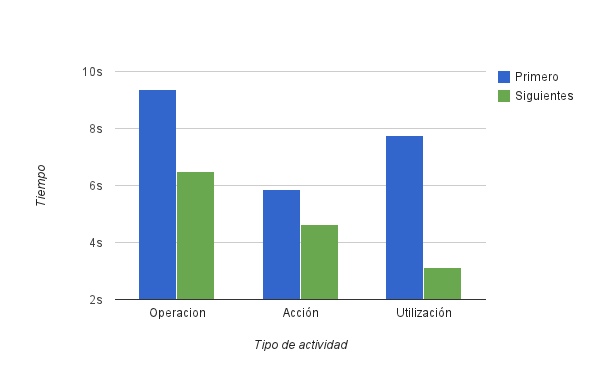
\includegraphics[width=14cm]{resultados/imagenes/interfaz_tiempo_actividades.png}
\caption{Tiempo por tipo de actividad}
\label{fig:interfaz_tiempo_acciones}
\end{figure}

En la figura~\ref{fig:interfaz_tiempo_acciones} se observa como en promedio el
usuario aprende, y en las siguientes acciones similares demora menos tiempo,
este es un factor importante y es el objetivo de esta prueba pues muestra que la
interfaz es fácil de usar, y con tres movimientos básicos, el usuario puede
utilizarla sin mayores inconvenientes. Se observa una mejoría del $30\%$ en las
acciones \emph{Menú Contextual}, $21\%$ en las acciones de tipo \emph{Menú de la
    Interfaz} y finalmente, una mejoría del $60\%$ en las acciones de tipo
\emph{Herramienta}.


La tabla~\ref{tab:interfaz_cantidad_espaciales} nos muestra la cantidad de
movimientos espaciales realizados por los usuarios, se observa que en promedio
se desplazaron $10,88$ veces por el escenario, y $6,75$ veces acercaron o
alejaron la cámara del paciente.

\observacion{Hay que dejar bien en claro de donde sale esto, por que es
importante entender el significado de esta diferencia}

\begin{table}[H]
\centering
\begin{tabular}{lrrr}
\toprule
\textbf{Jugador}  & \textbf{Movimiento} & \textbf{Zoom} & \textbf{Total} \\
\midrule
1        & 18         & 2    & 20 \\
2        & 7          & 8    & 15 \\
3        & 14         & 12   & 26 \\
4        & 9          & 14   & 23 \\
5        & 5          & 8    & 13 \\
6        & 14         & 4    & 18 \\
7        & 16         & 3    & 19 \\
8        & 4          & 3    &  7 \\
\midrule
\textbf{Promedio} & \textbf{10,88}      & \textbf{6,75} & \textbf{17,63} \\
\bottomrule
\end{tabular}
\caption{Cantidad de movimientos espaciales}
\label{tab:interfaz_cantidad_espaciales}
\end{table}

No existe una cantidad mínima o máxima que el usuario debería acercar o mover la
cámara, en cambio, los datos mostrados en~\ref{tab:interfaz_cantidad_espaciales},
muestran que no son necesarias demasiadas acciones, juntando esta información,
con la información proveída en la tabla~\ref{tab:interfaz_tiempo_total}, se ve
que en promedio los usuarios realizaron $1,7$ movimientos por minuto.

\begin{table}[!hbt]
\centering
\begin{tabular}{lrrr}
\toprule
\textbf{Alumno} & \textbf{Tiempo} \\
\midrule
1        & 8:32 \\
2        & 6:03 \\
3        & 8:33 \\
4        & 5:17 \\
5        & 6:55 \\
6        & 8:40 \\
7        & 7:03 \\
8        & 10:27 \\
\midrule
\textbf{Promedio} & \textbf{7:41} \\
\bottomrule
\end{tabular}
\caption{Tiempo de prueba por usuario}
\label{tab:interfaz_tiempo_total}
\end{table}

El tiempo total que se observa en la tabla~\ref{tab:interfaz_tiempo_total},
muestra que en promedio a cada alumno le tomo $7:41$ minutos realizar todos los
pasos especificados, es importante notar que este tiempo incluye el tiempo de
adaptación. 



\begin{table}[!hbt]
\centering
\begin{tabular}{lrrr}
\toprule
\textbf{Alumno} & \textbf{Pasos requeridos} \\
\midrule
1 & 19 \\
2 & 15 \\
3 & 18 \\
4 & 15 \\
5 & 18 \\
6 & 16 \\
7 & 19 \\
8 & 14 \\
\midrule
\textbf{Promedio} & \textbf{16,75} \\
\bottomrule
\end{tabular}
\caption{Acciones realizadas por usuario}
\label{tab:interfaz_acciones}
\end{table}

La tabla~\ref{tab:interfaz_acciones} nos muestra la cantidad de acciones que
realizaron los alumnos, junto con las acciones correctas para llevar a cabo el
procedimiento. Se observa que en promedio realizaron $16.75$ acciones correctas,
esto permite identificar en que parte de procedimiento los usuarios tienen
inconvenientes en cuanto al uso de la interfaz.

\subsection{Encuesta}

\fixme{Como fue descripta en la sección~\ref{sec:interfaz} la encuesta es
realizada a cada usuario}{Mejorar}, y es utilizada para obtener el grado de
disconformidad de los mismos. Se utiliza la disconformidad para resaltar los
puntos débiles, y así, aquellas variables que tengan el mayor porcentaje serán
las que deben ser arregladas.

Las preguntas que forman parte de la  encuesta son agrupadas en cuanto a
aspectos de calidad gráfica, interacción con el entorno, interacción con los
objetos, características del entorno, usabilidad de la interfaz e integración
con el hardware.

Luego de estas agrupaciones obtenemos el resultado que se muestra en la
tabla~\ref{tab:interfaz_disconformidad_metrica}. En esta tabla se puede observar
que las mayores disconformidades son con respecto a la usabilidad de la interfaz
que llega al $51\%$, la interacción de los usuarios con el entorno que llega al
$50\%$, la interacción con los objetos que llega al $49\%$. Luego, se pueden
observar también otras disconformidades con menor porcentaje, las
características del entorno con un  $33\%$, la integración con el hardware con
un  $27\%$ y por ultimo, la calidad gráfica con un  $17\%$.

\observacion{Hay que explicar que estas pruebas se hicieron de forma previa a
las demás y que se arreglan algunos casos}

\begin{table}[H]
\centering
\begin{tabular}{lr}
\toprule
Métrica & Disconformidad \\
\midrule
Calidad Gráfica         & 0.17 \\
Interacción Entorno     & 0.50\\
Interacción Objetos     & 0.49\\
Características Entorno & 0.33\\
Usabililidad Interfaz   & 0.51\\
Integración Hardware    & 0.27\\
\bottomrule
\end{tabular}
\caption{Disconformidad por métrica}
\label{tab:interfaz_disconformidad_metrica}
\end{table}

La conclusión de esta prueba de interfaz, es que si bien, pudo ser utilizada sin
mayores inconvenientes, existe un alto grado de disconformidad con la interfaz,
además cabe resaltar, los sujetos de prueba son personas acostumbradas al uso de
tecnologías similares. Otros puntos débiles encontrados en esta prueba son la
interacción con el entorno y  con los objetos.

Como resultado de esta prueba, la interfaz y la interacción con objetos y
elementos sufren modificaciones a fin de su utilización con usuarios no
técnicos.

Las demás pruebas mencionadas en este capítulo son realizadas con la versión
final de la solución, la cual es obtenida luego de las mejoras realizadas a los
puntos débiles detectados por esta prueba.

%! TEX root = ../main.tex


\section{Encuesta de Ubicación}
\label{sec:res_UBICACION}

Como se indicó en la sección~\ref{sec:ubicacion}, se agrupa a los alumnos
encuestados de acuerdo a las características de sus dispositivos móviles y del
acceso a internet.

En la figura~\ref{fig:ubicacion_acceso_internet} se puede observar que de 93
encuestados, el $94,6\%$ tiene acceso a internet al menos en algún momento y que
solo el $5.4\%$ no tiene acceso a internet en sus dispositivos móviles.

\begin{figure}[ht!]
\centering
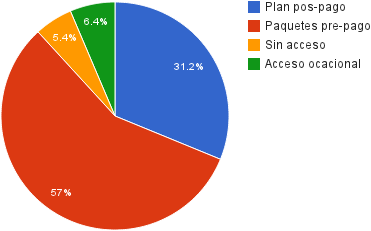
\includegraphics[scale=0.8]{resultados/imagenes/ubicacion_acceso_internet.png}
\caption{Acceso a internet desde dispositivos móviles}
\label{fig:ubicacion_acceso_internet}
\observacion{no habia otras caracteristicas}
\end{figure}

Por otro lado, en la figura\ref{fig:ubicacion_sistemas_operativos} se muestra
los sistemas operativos móviles utilizados por los usuarios encuestados. Se
puede observar que Android lidera con un $61.3\%$, le sigue Windows Phone con un
$12.9\%$.

\begin{figure}[ht!]
\centering
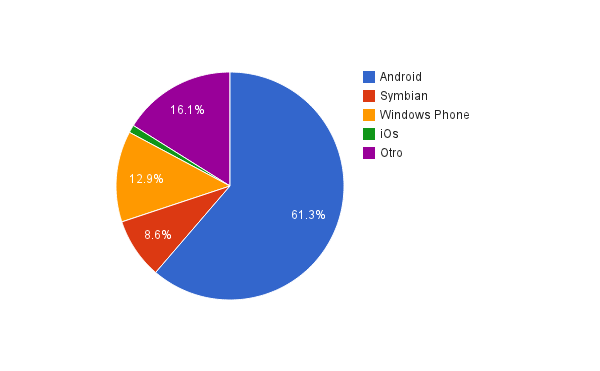
\includegraphics[scale=0.8]{resultados/imagenes/ubicacion_sistemas_operativos.png}
\caption{Sistemas operativos móviles utilizados}
\label{fig:ubicacion_sistemas_operativos}
\observacion{Meter a la par de otros}
\end{figure}

Por último, se discrimina a los encuestados para determinar cuantos de ellos
tiene dispositivos móviles que cumplen los requisitos mínimos para utilizar la
solución propuesta según lo descrito en la sección~\ref{sec:ubicacion}. En la
figura~\ref{fig:ubicacion_requisitos_minimos} se puede observar que el $18,3\%$
de los encuestados cumplen con los requisitos.

\begin{figure}[ht!]
\centering
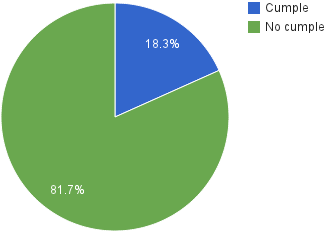
\includegraphics[scale=0.8]{resultados/imagenes/ubicacion_requisitos_minimos.png}
\caption{Dispositivos que cumplen con los requisitos mínimos para la prueba}
\label{fig:ubicacion_requisitos_minimos}
\observacion{Que conclusiones podría quitar de esto?}
\end{figure}

\observacion{Acercar más los gráficos}

%! TEX root = ../main.tex

\section{Encuesta Subjetiva}

En el análisis de los resultados de las encuestas subjetivas, existieron alumnos
que no respondieron todas las preguntas, para tratar este tipo de casos, es
importante analizar la naturaleza del patrón de datos
faltantes\cite{carpita2011imputation}. 

La información recogida por la encuesta muestra que hay datos faltantes, como se
explico en~\ref{sec:informacion_faltante}, esta información faltante es
completamente aleatoria en relación a la variable medida y a las demás
variables, de hecho, una sola encuesta tiene información faltante, así, se
establece que el tipo de información faltante es \emph{Información faltante
    completamente aleatoria}.

En su resumen de las diferentes técnicas y cuando se deben utilizar,
\cite{tsikriktsis2005review}, recomienda la utilización de la sustitución basada
en promedio por caso. Así, se completan los valores faltantes con el promedio de
respuestas completadas por el usuario.

\subsection{Resultados}

Se presentan a continuación los resultados de las encuestas, agrupados por los
factores definidos en~\ref{sec:variables}.

La tabla~\ref{tab:subjetiva_conformidad_exploracion} nos muestra las respuestas
de los alumnos a las preguntas relacionadas al factor exploración, son cuatro
preguntas, las cuales fueron descritas en~\ref{sec:sub_exploracion}. 

\begin{table}[!hbt]
\centering
\begin{tabular}{@{} *{5}{r} @{}}
\toprule
& \multicolumn{4}{c}{Exploración} \\
\cmidrule(lr){2-5}
Alumno &
\parbox{3cm}{Funciones realizadas por los elementos del juego} &
\parbox{3cm}{Aleatoriedad para afianzar conocimientos} &
\parbox{2.5cm}{Aleatoriedad para representar realismo} &
\parbox{2.5cm}{Facilidad de uso}  \\
\midrule
1         & 2   & 6   & 5   & 6  \\
2         & 6   & 6   & 4   & 6  \\
3         & 3   & 3   & 5   & 5  \\
4         & 6   & 6   & 6   & 6  \\
5         & 6   & 6   & 2   & 5  \\
6         & 6   & 6   & 6   & 6  \\
7         & 7   & 7   & 7   & 7  \\
8         & 6   & 6   & 7   & 7  \\
9         & 5   & 7   & 7   & 7  \\
10        & 6   & 7   & 6   & 6  \\
11        & 7   & 6   & 7   & 6  \\
\bottomrule
\end{tabular}
\caption{Resultados de la encuesta subjetiva relacionados al factor Exploración}
\label{tab:subjetiva_conformidad_exploracion}
\end{table}

La tabla~\ref{tab:subjetiva_conformidad_gamificacion} muestra las respuestas de
los alumnos a las preguntas relacionadas al factor \textit{Gamificación}, son
cinco preguntas, las cuales fueron descritas en~\ref{sec:sub_gamificacion}. 

\begin{table}[!hbt]
\centering
\begin{tabular}{@{} *{5}{r} @{}}
\toprule
& \multicolumn{4}{c}{Gamificación} \\
\cmidrule(lr){2-5}
Alumno &
\parbox{2.5cm}{Motivación del puntaje} &
\parbox{2.5cm}{Importancia del puntaje} &
\parbox{3cm}{Socialización de los puntajes} &
\parbox{3cm}{Medición del tiempo como motivación} \\
\midrule
1  & 6 & 4 & 4 & 7  \\
2  & 7 & 4 & 6 & 6  \\
3  & 6 & 6 & 5 & 6  \\
4  & 1 & 4 & 6 & 1  \\
5  & 2 & 2 & 7 & 7  \\
6  & 6 & 5 & 4 & 6  \\
7  & 7 & 7 & 6 & 7  \\
8  & 7 & 7 & 7 & 7  \\
9  & 7 & 7 & 7 & 7  \\
10 & 7 & 4 & 5 & 7  \\
11 & 5 & 4 & 5 & 6  \\
\bottomrule
\end{tabular}
\caption{Resultados de la encuesta subjetiva relacionados al factor Gamificación}
\label{tab:subjetiva_conformidad_gamificacion}
\end{table}

La tabla~\ref{tab:subjetiva_conformidad_inmersion} muestra las respuestas de
los alumnos a las preguntas relacionadas al factor \textit{Inmersión}, son
cinco preguntas, las cuales fueron descritas en~\ref{sec:sub_inmersion}. 

\begin{table}[!hbt]
\centering
\begin{tabular}{@{} *{6}{r} @{}}
\toprule
& \multicolumn{5}{c}{Inmersión} \\
\cmidrule(lr){2-6}
Alumno &
\parbox{2.5cm}{Escenografía para entrar en ambiente} &
\parbox{2.5cm}{Juegos cortos como ayuda para la repetición} &
\parbox{2.5cm}{Gráficos en tres dimensiones para entender el entorno} &
\parbox{2.5cm}{Realismo a través de ordenes verbales} &
\parbox{2.5cm}{Simulación como herramienta} \\
\midrule
1  & 4 & 6 & 4 & 5 & 3  \\
2  & 6 & 6 & 6 & 6 & 6  \\
3  & 6 & 6 & 6 & 5 & 6  \\
4  & 4 & 6 & 7 & 5 & 6  \\
5  & 6 & 6 & 5 & 6 & 6  \\
6  & 6 & 6 & 6 & 4 & 4  \\
7  & 7 & 7 & 7 & 7 & 7  \\
8  & 6 & 7 & 7 & 7 & 7  \\
9  & 6 & 7 & 7 & 7 & 7  \\
10 & 6 & 3 & 4 & 6 & 6  \\
11 & 5 & 3 & 5 & 5 & 4  \\
\bottomrule
\end{tabular}
\caption{Resultados de la encuesta subjetiva relacionados al factor Inmersión}
\label{tab:subjetiva_conformidad_inmersion}
\end{table}


La tabla~\ref{tab:subjetiva_conformidad_pedagogia} agrupa las respuestas de los
alumnos según el factor pedagógico, son tres preguntas, las cuales fueron
descritas en~\ref{sec:sub_pedagogia}. 

\begin{table}[!hbt]
\centering
\begin{tabular}{@{} *{4}{r} @{}}
\toprule
& \multicolumn{3}{c}{Pedagogía} \\
\cmidrule(lr){2-4}
Alumno &
\parbox{4cm}{La solución para memorizar y comprender el procedimiento} &
\parbox{4cm}{Falta de pistas como ayuda al aprendizaje} &
\parbox{4cm}{Suficiencia de los botones que indican acciones} \\
\midrule
1  & 6 & 6 & 6  \\
2  & 6 & 6 & 7  \\
3  & 4 & 6 & 6  \\
4  & 6 & 7 & 6  \\
5  & 7 & 5 & 6  \\
6  & 4 & 4 & 6  \\
7  & 7 & 6 & 7  \\
8  & 6 & 7 & 7  \\
9  & 7 & 7 & 7  \\
10 & 6 & 7 & 7  \\
11 & 5 & 6 & 5  \\
\bottomrule
\end{tabular}
\caption{Resultados de la encuesta subjetiva relacionados al factor Pedagogía}
\label{tab:subjetiva_conformidad_pedagogia}
\end{table}


La tabla~\ref{tab:subjetiva_conformidad_representacion} agrupa las respuestas de
los alumnos según la calidad de presentación, son cinco preguntas, las cuales
fueron descritas en~\ref{sec:sub_representacion}. 

\begin{table}[!hbt]
\centering
\begin{tabular}{@{} *{6}{r} @{}}
\toprule
& \multicolumn{5}{c}{Representación} \\
\cmidrule(lr){2-6}
Alumno &
\parbox{2.5cm}{Movimientos motrices del paciente} &
\parbox{2.5cm}{Movimientos oculares del paciente} &
\parbox{2.5cm}{Reacción verbal del paciente} &
\parbox{2.5cm}{Distinción entre los estados del paciente} &
\parbox{2.5cm}{Acciones las herramientas} \\
\midrule
1  & 6 & 6 & 2 & 5 & 2  \\
2  & 4 & 5 & 5 & 6 & 4  \\
3  & 5 & 3 & 3 & 3 & 3  \\
4  & 6 & 5 & 2 & 4 & 2  \\
5  & 2 & 2 & 6 & 6 & 6  \\
6  & 6 & 4 & 6 & 6 & 6  \\
7  & 7 & 6 & 5 & 7 & 5  \\
8  & 6 & 7 & 7 & 7 & 5  \\
9  & 5 & 6 & 2 & 7 & 6  \\
10 & 6 & 4 & 4 & 4 & 5  \\
11 & 6 & 4 & 6 & 6 & 5  \\
\bottomrule
\end{tabular}
\caption{Resultados de la encuesta subjetiva relacionados al factor
    Representación}
\label{tab:subjetiva_conformidad_representacion}
\end{table}


La tabla~\ref{tab:subjetiva_conformidad_retroalimentacion} agrupa las respuestas
de los alumnos según la calidad de retroalimentación, son tres preguntas, las
cuales fueron descritas en~\ref{sec:sub_retroalimentacion}. 

\begin{table}[!hbt]
\centering
\begin{tabular}{@{} *{4}{r} @{}}
\toprule
& \multicolumn{3}{c}{Retroalimentación} \\
\cmidrule(lr){2-4}
Alumno &
\parbox{4cm}{Detalles de los pasos realizados incorrectamente} &
\parbox{4cm}{Suficiencia de los detalles de los pasos realizados incorrectamente} &
\parbox{4cm}{Iconos para representar el estado del jugador} \\
\midrule
1  & 3 & 2 & 7  \\
2  & 5 & 4 & 6  \\
3  & 3 & 6 & 6  \\
4  & 6 & 6 & 6  \\
5  & 6 & 1 & 6  \\
6  & 2 & 6 & 6  \\
7  & 6 & 7 & 7  \\
8  & 6 & 6 & 7  \\
9  & 6 & 6 & 7  \\
10 & 5 & 4 & 6  \\
11 & 4 & 5 & 6  \\
\bottomrule
\end{tabular}
\caption{Resultados de la encuesta subjetiva relacionados al factor
    Retroalimentación}
\label{tab:subjetiva_conformidad_retroalimentacion}
\end{table}


La tabla~\ref{tab:subjetiva_conformidad_utilidad} agrupa las respuestas de los
alumnos según la utilidad de la solución, son tres preguntas, las cuales fueron
descritas en~\ref{sec:sub_utilidad}. 


\begin{table}[!hbt]
\centering
\begin{tabular}{@{} *{6}{r} @{}}
\toprule
& \multicolumn{3}{c}{Utilidad} \\
\cmidrule(lr){2-4}
Alumno &
\parbox{4cm}{Simulación para complementar el estudio en clase y laboratorio} &
\parbox{4cm}{Simulación provee más facilidades para el estudio} &
\parbox{4cm}{Interacción con el paciente} \\
\midrule
1  & 7 & 5 & 7  \\
2  & 6 & 6 & 6  \\
3  & 6 & 6 & 6  \\
4  & 2 & 6 & 6  \\
5  & 2 & 6 & 6  \\
6  & 6 & 6 & 6  \\
7  & 7 & 6 & 7  \\
8  & 5 & 6 & 7  \\
9  & 7 & 7 & 7  \\
10 & 1 & 7 & 7  \\
11 & 6 & 4 & 5  \\
\bottomrule
\end{tabular}
\caption{Resultados de la encuesta subjetiva relacionados al factor Utilidad}
\label{tab:subjetiva_conformidad_utilidad}
\end{table}

\section{Agrupamiento de datos}

Los resultados se resumen en la tabla~\ref{tab:subjetiva_conformidad_resumen},
se muestra el número de alumno para identificar a un alumno y el promedio de sus
respuestas en la encuesta, se muestra el promedio de las mismas.

\begin{table}[!hbt]
\begin{tabular}{llllllllr}
\toprule
\textbf{\shortstack{Número de \\alumno}}         &
\begin{sideways}\textbf{Gamificación}                    \end{sideways}        &
\begin{sideways}\textbf{Exploración}                     \end{sideways}        &
\begin{sideways}\textbf{Inmersión}                       \end{sideways}        &
\begin{sideways}\textbf{Pedagogía}                       \end{sideways}        &
\begin{sideways}\textbf{Representación}                  \end{sideways}        &
\begin{sideways}\textbf{Retroalimentación}               \end{sideways}        &
\begin{sideways}\textbf{Utilidad}                        \end{sideways}        &
\textbf{\shortstack{Promedio\\de respuestas}}\\
\midrule
1              & 5 & 5 & 4 & 6 & 4 & 4 & 6 & 5 \\
2              & 6 & 6 & 6 & 6 & 5 & 5 & 6 & 6 \\
3              & 4 & 6 & 6 & 5 & 3 & 5 & 6 & 5 \\
4              & 6 & 3 & 6 & 6 & 4 & 6 & 5 & 5 \\
5              & 5 & 5 & 6 & 6 & 4 & 4 & 5 & 5 \\
6              & 6 & 5 & 5 & 5 & 6 & 5 & 6 & 5 \\
7              & 7 & 7 & 7 & 7 & 6 & 7 & 7 & 7 \\
8              & 7 & 7 & 7 & 7 & 6 & 6 & 6 & 7 \\
9              & 7 & 7 & 7 & 7 & 5 & 6 & 7 & 6 \\
10             & 6 & 6 & 5 & 7 & 5 & 5 & 5 & 5 \\
11             & 7 & 5 & 4 & 5 & 5 & 5 & 5 & 5 \\
\midrule
Promedio Total & 6 & 6 & 6 & 6 & 5 & 5 & 6 & 6 \\
\bottomrule
\end{tabular}
\caption{Resultados de la encuesta subjetiva}
\label{tab:subjetiva_conformidad_resumen}
\end{table}

Se observa que el el puntaje más bajo en el promedio final es 5 que significa
\textit{Parcialmente de acuerdo}, y el más alto es 7, que significa
\textit{Totalmente de acuerdo}, se observa además el puntaje 6, que significa
\textit{De acuerdo}. 


Como se explica en la sección~\ref{sec:likert}, estos resultados están sujetos a
tendencias, para ello se aplica el método de doble
estandarización\cite{Pagolu2011}.

Con el resultado final de la estandarización diferenciamos cuales son los puntos
fuertes y cuales los puntos débiles de la solución propuesta con respecto a las
respuestas dadas por los usuarios. Estos valores son relativos a las respuestas
originales dadas en la encuesta, los resultados se muestran en la
tabla~\ref{tab:subjetiva_conformidad_corregida}.

\begin{table}[!hbt]
\centering
\begin{tabular}{lrrrrrrrr}
\toprule
\textbf{\shortstack{Número de \\alumno}}                                &
\begin{sideways}\textbf{Gamificación}                    \end{sideways} &
\begin{sideways}\textbf{Exploración}                     \end{sideways} &
\begin{sideways}\textbf{Inmersión}                       \end{sideways} &
\begin{sideways}\textbf{Pedagogía}                       \end{sideways} &
\begin{sideways}\textbf{Representación}                  \end{sideways} &
\begin{sideways}\textbf{Retroalimentación}               \end{sideways} &
\begin{sideways}\textbf{Utilidad}                        \end{sideways} &
\textbf{\shortstack{Promedio\\de respuestas}}\\
\midrule
1              & 0.45 & 0.55 & 0.20 & 0.63 & 0.44 & 0.41 & 0.82 & 0.47 \\
2              & 0.33 & 0.53 & 0.49 & 0.61 & 0.27 & 0.13 & 0.52 & 0.41 \\
3              & 0.17 & 0.86 & 0.87 & 0.67 & 0.13 & 0.67 & 1.00 & 0.60 \\
4              & 0.75 & 0.31 & 0.63 & 0.81 & 0.47 & 0.78 & 0.54 & 0.59 \\
5              & 0.46 & 0.58 & 0.69 & 0.67 & 0.57 & 0.50 & 0.54 & 0.58 \\
6              & 1.00 & 0.73 & 0.68 & 0.42 & 0.90 & 0.67 & 1.00 & 0.78 \\
7              & 1.00 & 0.79 & 1.00 & 0.67 & 0.50 & 0.87 & 0.78 & 0.80 \\
8              & 0.75 & 1.00 & 0.83 & 0.75 & 0.70 & 0.70 & 0.44 & 0.75 \\
9              & 0.90 & 1.00 & 0.93 & 1.00 & 0.64 & 0.92 & 1.00 & 0.90 \\
10             & 0.79 & 0.74 & 0.54 & 0.92 & 0.60 & 0.60 & 0.67 & 0.68 \\
11             & 0.75 & 0.42 & 0.08 & 0.25 & 0.60 & 0.35 & 0.25 & 0.39 \\
\midrule
\textbf{Promedio Total} & 0.67 & 0.68 & 0.63 & 0.67 & 0.53 & 0.60 & 0.69 & 0.63 \\
\bottomrule
\end{tabular}
\caption{Resultados de la encuesta subjetiva con doble estandarización}
\label{tab:subjetiva_conformidad_corregida}
\end{table}

Para obtener una mejor visión de las fortalezas y debilidades de la solución
propuesta, se presenta el gráfico de kiviat~\ref{fig:subjetiva_kiviat}, en la
misma se puede observar cuales son los puntos débiles de la solución.

\begin{figure}[!ht]
\begin{tikzpicture}[label distance=.15cm]
\tkzKiviatDiagram[radial=2,
                    lattice=2, step=2,
                    scale=2.3]%
                {Gamificación,
                 Exploración,
                 Inmersión,
                 Pedagogía,
                 Representación,
                 Retroalimentación,
                 Utilidad}
\tkzKiviatLine[thick,
                color=blue,
                mark=ball,
                ball color=red,
                mark size=1pt,opacity=.2, 
                fill=red!20](0.67,0.68,0.63,0.67,0.53,0.60,0.69)
\end{tikzpicture}
\label{fig:subjetiva_kiviat}
\caption{Gráfico de Kiviat de los factores evaluados}
\end{figure}

En el gráfico se observa en la figura, que las principales debilidades de
la solución son la representación y la retroalimentación.

Es importante notar que los datos la figura~\ref{fig:subjetiva_kiviat}
y~\ref{tab:subjetiva_conformidad_corregida} son relativas a los datos de la
tabla~\ref{tab:subjetiva_conformidad_resumen}, es decir, que la representación
es el punto más débil, pero se ve en~\ref{tab:subjetiva_conformidad_resumen}
que el valor es 5 de 7, lo que indica que es un punto aceptable, y entre
los factores analizados es el que menos aprobación obtuvo.



\subsection{Correlacion}

En la tabla~\ref{tab:subjetiva_correlacion} se muestra la correlación entre los
factores analizados, las mismas fueron calculadas según lo explicado en la
sección \todox{Agregar sección de correlación}. En resumen se pueden notar las
siguientes correlaciones:

\begin{itemize}
\item \textbf{Gamification y Exploración, 0.33} Correlación positiva moderada.
\item \textbf{Gamification y Pedagogía, 0.27} Correlación positiva débil.
\item \textbf{Gamificatoin e Inmersión, 0.48} Correlación positiva fuerte.
\item \textbf{Gamification y Representación, 0.81} Correlación positiva muy fuerte.
\item \textbf{Gamification y Retroalimentación, 0.66} Correlación positiva fuerte.
\item \textbf{Gamification y Utilidad, 0.26} Correlación positiva débil.
\item \textbf{Exploración y Pedagogía, 0.52} Correlación positiva fuerte.
\item \textbf{Exploración e Inmersión, 0.53} Correlación positiva fuerte.
\item \textbf{Exploración y Representación, 0.44} Correlación positiva fuerte.
\item \textbf{Exploración y Retroalimentación, 0.37} Correlación positiva moderada.
\item \textbf{Exploración y Utilidad, 0.69} Correlación positiva fuerte.
\item \textbf{Pedagogía e Inmersión, 0.57} Correlación positiva fuerte.
\item \textbf{Pedagogía y Representación, 0.23} Correlación positiva débil.
\item \textbf{Pedagogía y Retroalimentación, 0.68} Correlación positiva fuerte.
\item \textbf{Pedagogía y Utilidad, 0.54} Correlación positiva fuerte.
\item \textbf{Inmersión y Representación, 0.39} Correlación positiva moderada.
\item \textbf{Inmersión y Retroalimentación, 0.49} Correlación positiva fuerte.
\item \textbf{Inmersión y Utilidad, 0.35} Correlación positiva moderada.
\item \textbf{Representación y Retroalimentación, 0.51} Correlación positiva fuerte.
\item \textbf{Representación y Utilidad, 0.36} Correlación positiva moderada.
\item \textbf{Retroalimentación y Utilidad, 0.52} Correlación positiva fuerte.
\end{itemize}

\begin{table}[!hbt]
\centering
\begin{tabular}{l|lllllllr}
\toprule
        &
\begin{sideways}\textbf{Gamificación}                    \end{sideways}        &
\begin{sideways}\textbf{Exploración}                     \end{sideways}        &
\begin{sideways}\textbf{Inmersión}                       \end{sideways}        &
\begin{sideways}\textbf{Pedagogía}                       \end{sideways}        &
\begin{sideways}\textbf{Representación}                  \end{sideways}        &
\begin{sideways}\textbf{Retroalimentación}               \end{sideways}        &
\begin{sideways}\textbf{Utilidad}                        \end{sideways}      \\
\midrule
\textbf{Gamification}      & 1    & 0.33 & 0.27 & 0.48 & 0.81 & 0.66  & 0.27 \\
\textbf{Exploración}       & 0.33 & 1    & 0.52 & 0.53 & 0.44 & 0.37  & 0.69 \\
\textbf{Inmersión}         & 0.27 & 0.52 & 1    & 0.57 & 0.23 & 0.68  & 0.54 \\
\textbf{Pedagogía}         & 0.48 & 0.53 & 0.57 & 1    & 0.39 & 0.49  & 0.35 \\
\textbf{Representación}    & 0.81 & 0.44 & 0.23 & 0.39 & 1    & 0.51  & 0.36 \\
\textbf{Retroalimentación} & 0.66 & 0.37 & 0.68 & 0.49 & 0.51 & 1     & 0.52 \\
\textbf{Utilidad}          & 0.27 & 0.69 & 0.54 & 0.35 & 0.36 & 0.52  & 1 \\
\bottomrule
\end{tabular}
\caption{Correlación entre los factores analizados} 
\label{tab:subjetiva_correlacion}
\end{table}

\section{Encuesta Objetiva}
\label{sec:res_OBJETIVA}

Como se detalló en la sección~\ref{sec:objetiva}, la encuesta realizada a cada
usuario, parte del experimento, es utilizada para obtener una comparación en
cuanto al rendimiento de los usuarios que forman parte de la muestra y los que
forman parte del grupo de control.

La tabla~\ref{tab:objetiva_rendimiento_por_pregunta} muestra el nivel de acierto
en promedio por pregunta de los usuarios que forman parte de la muestra y de los que
forman parte del grupo de control, con sus respectivas desviaciones estándar. Según
estos datos, en el $60\%$ de los casos hay una leve mejoría en cuanto al nivel de acierto
para los usuarios que forman parte de la muestra.

\begin{table}[!hbt]
\centering
\begin{tabular}{|l|r|r|r|r|}
\hline
\rowcolor{gris} 
\textbf{Pregunta} & 
\textbf{Prom. Jugó} & 
\textbf{Des. Jugó} & 
\textbf{Prom. No Jugó} & 
\textbf{Des. No Jugó} \\
\hline
1 & 0.36 & 0.50 & 0.18 & 0.39 \\
\hline
2 & 0.64 & 0.50 & 0.60 & 0.49 \\
\hline
3 & 0.09 & 0.30 & 0.14 & 0.34 \\
\hline
4 & 0.27 & 0.47 & 0.25 & 0.44 \\
\hline
5 & 0.82 & 0.40 & 0.56 & 0.50 \\
\hline
6 & 0 & 0 & 0.18 & 0.39 \\
\hline
7 & 0.64 & 0.50 & 0.51 & 0.50 \\
\hline
8 & 0.45 & 0.52 & 0.27 & 0.45 \\
\hline
9 & 0.18 & 0.40 & 0.32 & 0.47 \\
\hline
10 & 0.36 & 0.50 & 0.45 & 0.50 \\
\hline
\end{tabular}
\caption{Rendimiento promedio de usuarios por pregunta}
\label{tab:objetiva_rendimiento_por_pregunta}
\end{table}

Los datos mostrados sólo sugieren levemente una tendencia a la mejoría de los puntajes 
para los usuarios que forman parte de la muestra, sin embargo, estos datos no pueden ser 
tomados para realizar conclusiones ya que la cantidad de sesiones de juego por usuario no 
se considera suficiente para que el uso de la solución propuesta afecte realmente en el 
aprendizaje del mismo.

\section{Registro de actividad}

\martin{Ponemos a los alumnos que no jugaron con 0 partidas y 0 segundos, o
    los omitimos?}

Las actividad de los usuarios es registrada y almacenada para su análisis, a
continuación se presentan los resultados de ese análisis, el mismo fue descrito
en~\ref{sec:registro}.


\begin{table}[!hbt]
\centering
\begin{tabular}{lrrrrrrrr}
\toprule
                   & \multicolumn{2}{c}{Extracción de sangre} \\
                   \cmidrule(lr){2-3} 
Número de alumno   & Sesiones jugadas                            & Tiempo jugado \\
\midrule
 1       & 5  & 1202 \\
 2       & 19 & 2507 \\
 4       & 5  & 398  \\
 5       & 6  & 768  \\
 6       & 17 & 2371 \\
 7       & 7  & 707  \\
 9       & 1  & 126  \\
10       & 8  & 960  \\
\midrule
Total:   & 68 & 9039 \\
\bottomrule
\end{tabular}
\caption{Número de partidas y tiempo total por alumno, en la escena de
    extracción de sangre.}
\label{tab:log_hemocultivo_partida}
\end{table}

La cantidad de partidas jugadas por usuario, se ven en la
tabla~\ref{tab:log_hemocultivo_partida}, se observa que existen 3 alumnos que no
participaron del experimento o no se registro su actividad.

Los registros pueden no ser registrados sí
\begin{enumerate*}[label=\itshape\alph*\upshape)]
    \item El usuario utilizo la solución, pero no envió los datos y, luego
        desinstalo la solución o borro los datos de la misma, o,
    \item El usuario no utilizo la solución.
\end{enumerate*}

En la tabla~\ref{tab:log_glasgow_random_partida}, se observa la cantidad de
sesiones y tiempo total por alumno, en la escena de \textit{Glasgow}, en modo de
evaluación.

Se observa que $5$ alumnos participaron en $22$ sesiones, en total jugaron
$1768$ segundos.

\begin{table}[!hbt]
\centering
\begin{tabular}{lrrrrrrrr}
\toprule
& \multicolumn{2}{c}{Glasgow (Evaluación)} \\
                   \cmidrule(lr){2-3} 
Número de alumno   & Sesiones jugadas                            & Tiempo jugado \\
\midrule
1     & 4  & 211 \\
2     & 8  & 738 \\
4     & 3  & 132 \\
6     & 1  & 97  \\
7     & 6  & 590 \\
\midrule
Total & 22 & 1768 \\
\bottomrule
\end{tabular}
\caption{Número de partidas y tiempo total por alumno, en la escena
    \textit{Glasgow}, en modo evaluación}
\label{tab:log_glasgow_random_partida}
\end{table}


\begin{table}[!hbt]
\centering
\begin{tabular}{lrrrrrrrr}
\toprule
& \multicolumn{2}{c}{Glasgow (Exploración)} \\
                   \cmidrule(lr){2-3} 
Número de alumno   & Sesiones jugadas                            & Tiempo jugado \\
\midrule
1        & 2 & 79 \\
2        & 3 & 80 \\
4        & 3 & 89 \\
6        & 1 & 79 \\
\midrule
Total:   & 9 & 327 \\
\bottomrule
\end{tabular}
\caption{Número de partidas y tiempo total por alumno, en la escena
    \textit{Glasgow}, en modo exploración}
\label{tab:log_glasgow_custom_partida}
\end{table}


En las tablas \ref{tab:log_hemocultivo_puntaje} y \ref{tab:log_glasgow_random_puntaje} se muestran los primeros puntajes y 
un promedio de los puntajes siguientes obtenidos por cada usuario en los procedimientos de extracción de sangre y de la 
evaluación de la escala de Glasgow. Se debe tener en cuenta el tiempo y las cantidades de veces que cada alumno jugó
cada uno de los procedimientos para valorar los resultados mostrados. En general, los puntajes no muestran una mejora 
importante en los puntajes.

\begin{table}[!hbt]
\centering
\begin{tabular}{lrrrrrrrr}
\toprule
                   & \multicolumn{2}{c}{Extracción de sangre} \\
                   \cmidrule(lr){2-3} 
Número de alumno   & Primer Puntaje                            & Siguientes Puntajes \\
\midrule
 1       & 18  & 13.5 \\
 2       & 9 & 10.6 \\
 4       & 3 & 3.3 \\
 5       & 3 & 6.8  \\
 6       & 3 & 5.8 \\
 7       & 4 & 4 \\
 9       & 16  &  \\
10       & 3 & 7.2 \\
\bottomrule
\end{tabular}
\caption{Puntaje obtenido la primera vez y el promedio de las siguientes veces por alumno, en la escena de
    extracción de sangre.}
\label{tab:log_hemocultivo_puntaje}
\end{table}


\begin{table}[!hbt]
\centering
\begin{tabular}{lrrrrrrrr}
\toprule
& \multicolumn{2}{c}{Glasgow (Evaluación)} \\
                   \cmidrule(lr){2-3} 
Número de alumno   & Primer Puntaje                            & Siguientes Puntajes \\
\midrule
1     & 1 & 1.5 \\
2     & 2 & 2.3 \\
4     & 1 & 1.5 \\
6     & 2 & 2 \\
7     & 0 & 1 \\
\bottomrule
\end{tabular}
\caption{Puntaje obtenido la primera vez y el promedio de las siguientes veces por alumno, en la escena
    \textit{Glasgow}, en modo evaluación}
\label{tab:log_glasgow_random_puntaje}
\end{table}

\section{Correlación entre variables}

% Datos globales
En la tabla~\ref{tab:all_correlation} se observa la correlación entre cinco
variables estudiadas, a fin de observar si existe alguna correlación entre los
valores, se utiliza la correlación de \emph{Pearson}, descrita
en~\ref{sec:correlacion}.

\begin{table}[H]
\centering
\begin{tabular}{lrrrrrr}
\toprule
        &
\begin{sideways}\textbf{Tiempo de Uso}\end{sideways}             &
\begin{sideways}\textbf{Encuesta subjetiva}\end{sideways}        &
\begin{sideways}\textbf{Encuesta objetiva}\end{sideways}         &
\begin{sideways}\textbf{Puntaje Máximo Extracción}\end{sideways} &
\begin{sideways}\textbf{Puntaje Máximo Glasgow}\end{sideways}    \\
\midrule
Tiempo de Uso             & 1    & -0.2  & 0.15  & 0.62 & 0.41 & 0.78 \\
Encuesta subjetiva        & -0.2 & 1     & -0.07 & 0.04 & 0.11 & -0.28\\
Encuesta objetiva         & 0.15 & -0.07 & 1     & 0.44 & 0.44 & 0.02 \\
Puntaje máximo Extracción & 0.62 & 0.04  & 0.44  & 1    & 0.96 & 0.44 \\
Puntaje máximo Glasgow    & 0.41 & 0.11  & 0.44  & 0.96 & 1    & 0.27 \\
\bottomrule               & 0.78 & -0.28 & 0.02  & 0.44 & 0.27 & 1    \\
\end{tabular}
\caption{Correlación entre factores estudiados} 
\label{tab:all_correlation}
\end{table}

Las correlaciones fuertes, que se observan en la
tabla~\ref{tab:all_correlation}, son:

\begin{itemize}
    \item Tiempo de uso y puntaje máximo extracción, $0,62$, correlación
        positiva fuerte.
    \item Tiempo de uso y puntaje máximo Glasgow, $0,78$, correlación positiva
        muy fuerte.
    \item Puntaje máximo extracción y encuesta objetiva, $0,44$, correlación
        positiva fuerte.
\end{itemize}


La tabla~\ref{tab:all_correlation} indica que existe una correlación positiva
fuerte ($0,62$ y $0,78$) entre el tiempo de uso y el puntaje más alto obtenido,
lo que sugiere que mientras más se utiliza la solución, se obtienen mejores
resultados. 

Una correlación positiva fuerte entre el puntaje máximo obtenido en la
Extracción y la encuesta objetiva ($0,44$), sugiere que existe una relación entre
el nivel de conocimientos de los alumnos y su desempeño en la práctica.


%\section{Objetivos}
\label{sec:resultados_objetivos}

Esta sección presenta un resumen de los resultados de los objetivos propuestos
para la evaluación en la sección~\label{sec:evaluacion_objetivos}. 

\subsection{Validar las hipótesis asumidas durante el desarrollo de la solución}

En la tabla~\ref{tab:resultado_resumen_hipotesis} se observa la opinion de los
alumnos con respecto a las hipótesis asumidas en~\ref{sec:hipotesis}. Se observa
una aceptación a las hipótesis asumidas.

\begin{table}[!hbt]
\centering
\begin{tabular}{lcr}
\toprule
Hipótesis                        & Promedio Subjetiva      & Promedio estandarizado \\
\midrule
Comandos de voz con interfaz     & De acuerdo              & $0,55$ \\
Extracción uniforme de elementos & Parcialmente de acuerdo & $0,65$ \\
Acciones de bioseguridad         & De acuerdo              & $0,58$ \\
Representación iconográfica      & Parcialmente de acuerdo & $0,53$ \\
Factores motivadores             & De acuerdo              & $0,65$ \\
Falta de pistas                  & De acuerdo              & $0,61$ \\
\bottomrule
\end{tabular}
\caption{Hipótesis con su aceptación}\label{tab:resultado_resumen_hipotesis}
\end{table}


\subsection{Evaluar los puntos fuertes y débiles de la solución}

Utilizando los datos con doble estandarización de la
tabla~\ref{tab:subjetiva_conformidad_corregida}, se crea la
tabla~\ref{tab:resultado_resumen_aspectos_aceptacion}, donde se observa la
apreciación de los usuarios por cada aspecto estudiado.

\begin{table}[!hbt]
\centering
\begin{tabular}{lcr}
\toprule
Hipótesis         & Promedio Subjetiva      & Promedio estandarizado \\
\midrule
Motivación        & De acuerdo              & $0.67$  \\
Exploración       & De acuerdo              & $0.68$  \\
Inmersión         & De acuerdo              & $0.63$  \\
Pedagogía         & De acuerdo              & $0.67$  \\
Representación    & Parcialmente de acuerdo & $0.53$  \\
Retroalimentación & Parcialmente de acuerdo & $0.60$  \\
Utilidad          & De acuerdo              & $0.69$  \\
\bottomrule
\end{tabular}
\caption{Aceptación por aspecto de la solución}
\label{tab:resultado_resumen_aspectos_aceptacion}
\end{table}

Para  obtener una mejor visión de las fortalezas y debilidades de la solución
propuesta, se presenta el gráfico de \emph{kiviat}~\ref{fig:subjetiva_kiviat},
en la misma se puede observar cuales son los puntos débiles de la solución.

\begin{figure}[!ht]
\begin{tikzpicture}[label distance=.15cm]
\tkzKiviatDiagram[radial=2,
                    lattice=2, step=2,
                    scale=2.3]%
                {Motivación,
                 Exploración,
                 Inmersión,
                 Pedagogía,
                 Representación,
                 Retroalimentación,
                 Utilidad}
\tkzKiviatLine[thick,
                color=blue,
                mark=ball,
                ball color=red,
                mark size=1pt,opacity=.2, 
                fill=red!20](0.67,0.68,0.63,0.67,0.53,0.60,0.69)
\end{tikzpicture}
\label{fig:subjetiva_kiviat}
\caption{Gráfico de Kiviat de los factores evaluados}
\end{figure}

Se observa que las principales debilidades de la solución son la representación
y la retroalimentación, y las fortalezas la utilidad, pedagogía, exploración, y
la motivación.

\subsection{Determinar el nivel de aceptación de la solución}

En la sección~\ref{sec:res_subjetiva_abiertas} se muestra un resumen de la
apreciación de los alumnos hacia la solución, en este punto se observa que el
$100\%$ de los alumnos cree que es beneficioso contar con este tipo de
soluciones.


\subsection{Evaluar la utilización de la solución, y el progreso de los
    usuarios}

Se observa en las tablas~\ref{tab:log_hemocultivo_puntaje}
y~\ref{tab:log_glasgow_random_puntaje} los alumnos que participaron de la prueba
mejoran su desempeño a medida que aumenta el número de partidas. 

Es importante notar que la cantidad de partidas no es uniforme entre los
alumnos, es decir hay alumnos con más de $10$ partidas y usuarios con menos de
$5$, por ello, es difícil demostrar que existe un progreso a medida que aumenta
el número de partidas.

\subsection{Identificar la influencia de la utilización de la solución en el ámbito
    pedagógico}

Los datos mostrados en la sección~\ref{sec:res_objetiva} sólo sugieren levemente
una tendencia a la mejoría de los puntajes para los usuarios que forman parte de
la muestra, sin embargo, estos datos no pueden ser tomados para realizar
conclusiones ya que la cantidad de sesiones de juego por usuario no se considera
suficiente para que el uso de la solución propuesta afecte realmente en el
aprendizaje del mismo.

\subsection{Determinar correlaciones entre variables estudiadas}

% Datos globales
En la tabla~\ref{tab:all_correlation} se observa la correlación entre cinco
variables estudiadas, a fin de observar si existe alguna correlación entre los
valores, se utiliza la correlación de \emph{Pearson}, descrita
en~\ref{sec:correlacion}.

\begin{table}[H]
\centering
\begin{tabular}{lrrrrrr}
\toprule
        &
\begin{sideways}\textbf{Tiempo de Uso}\end{sideways}             &
\begin{sideways}\textbf{Encuesta subjetiva}\end{sideways}        &
\begin{sideways}\textbf{Encuesta objetiva}\end{sideways}         &
\begin{sideways}\textbf{Puntaje Máximo Extracción}\end{sideways} &
\begin{sideways}\textbf{Puntaje Máximo Glasgow}\end{sideways}    \\
\midrule
Tiempo de Uso             & 1    & -0.2  & 0.15  & 0.62 & 0.41 & 0.78 \\
Encuesta subjetiva        & -0.2 & 1     & -0.07 & 0.04 & 0.11 & -0.28\\
Encuesta objetiva         & 0.15 & -0.07 & 1     & 0.44 & 0.44 & 0.02 \\
Puntaje máximo Extracción & 0.62 & 0.04  & 0.44  & 1    & 0.96 & 0.44 \\
Puntaje máximo Glasgow    & 0.41 & 0.11  & 0.44  & 0.96 & 1    & 0.27 \\
\bottomrule               & 0.78 & -0.28 & 0.02  & 0.44 & 0.27 & 1    \\
\end{tabular}
\caption{Correlación entre factores estudiados} 
\label{tab:all_correlation}
\end{table}

Las correlaciones fuertes, que se observan en la
tabla~\ref{tab:all_correlation}, son:

\begin{itemize}
    \item Tiempo de uso y puntaje máximo extracción, $0,62$, correlación
        positiva fuerte.
    \item Tiempo de uso y puntaje máximo Glasgow, $0,78$, correlación positiva
        muy fuerte.
    \item Puntaje máximo extracción y encuesta objetiva, $0,44$, correlación
        positiva fuerte.
\end{itemize}


La tabla~\ref{tab:all_correlation} indica que existe una correlación positiva
fuerte ($0,62$ y $0,78$) entre el tiempo de uso y el puntaje más alto obtenido,
lo que sugiere que mientras más se utiliza la solución, se obtienen mejores
resultados. 

Una correlación positiva fuerte entre el puntaje máximo obtenido en la
Extracción y la encuesta objetiva ($0,44$), sugiere que existe una relación entre
el nivel de conocimientos de los alumnos y su desempeño en la práctica.



% TODO:

%   Ver lo de si se mantiene lo de relación objetiva-logs
%   Cambiar la sección de preguntas abiertas para poner una lista con
%   conclusiones por con porcentajes.


\printbibliography

\end{document}


